\documentclass[svgnames]{beamer}

\usetheme{Dresden}
\usecolortheme{beaver}

\usepackage{import, fancybox, graphicx, color, colortbl, bm}

\newcommand{\ssline}{\vspace{8 pt}}

\title{TCP ex Machina: \\Computer-Generated Congestion Control}

\author{Keith~Winstein and Hari~Balakrishnan}
\institute{MIT Computer Science and Artificial Intelligence Laboratory\\\vspace{\baselineskip}\textcolor{DarkBlue}{http://web.mit.edu/remy}}
\date{August 14, 2013}

\begin{document}

\begin{frame}[plain]

\titlepage

\end{frame}

\institute{MIT Computer Science and Artificial Intelligence Laboratory}

\section{Introduction}

\begin{frame}
\frametitle{Congestion control!}

\begin{itemize}

\Large

\item Prevents congestion collapse

\item Allocates network resources among users

\item Can be purely end-to-end or not

\end{itemize}

\end{frame}

\begin{frame}
\frametitle{The march of congestion control mechanisms}
\only<1>{\noindent \hspace{-.75 cm} 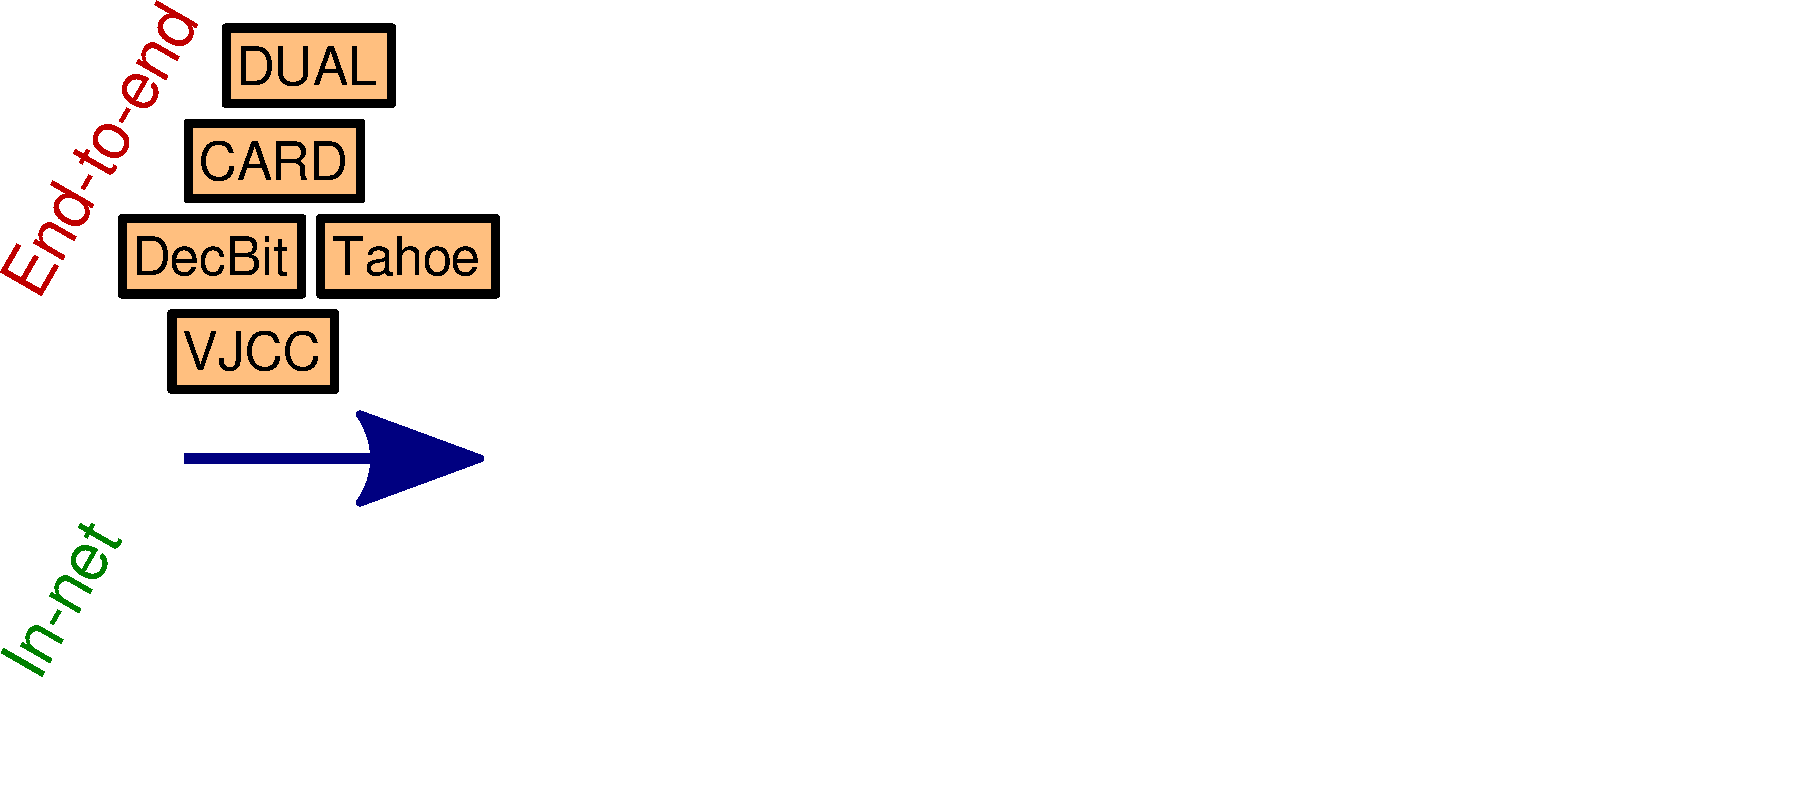
\includegraphics[width=1.1\textwidth]{march-4.pdf}

}
\only<2>{\noindent \hspace{-.75 cm} 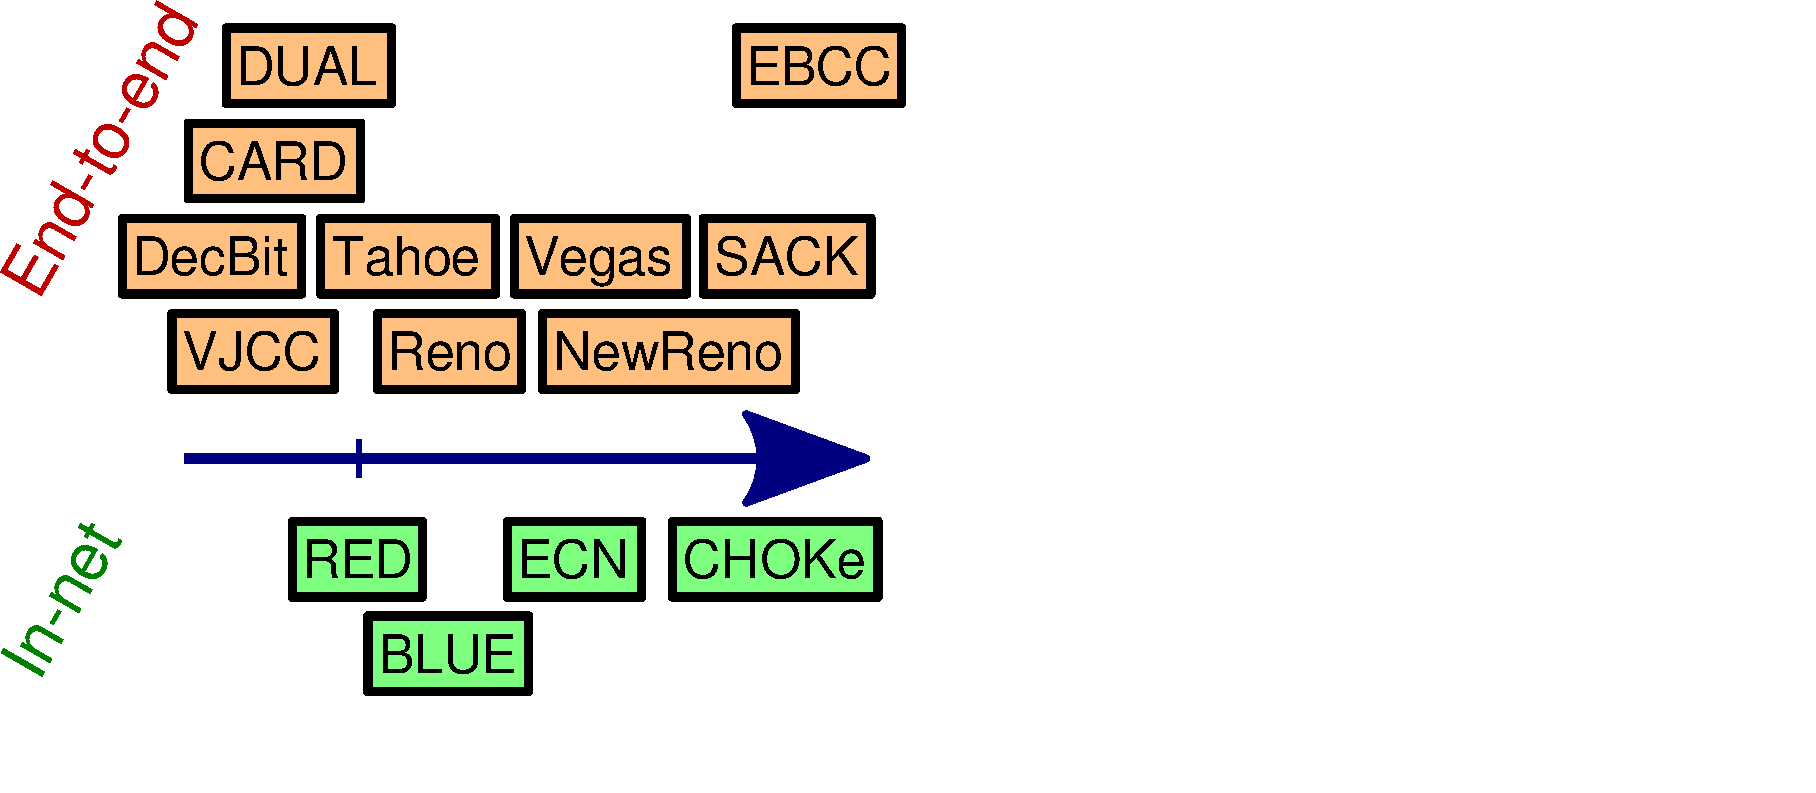
\includegraphics[width=1.1\textwidth]{march-3.pdf}

}
\only<3>{\noindent \hspace{-.75 cm} 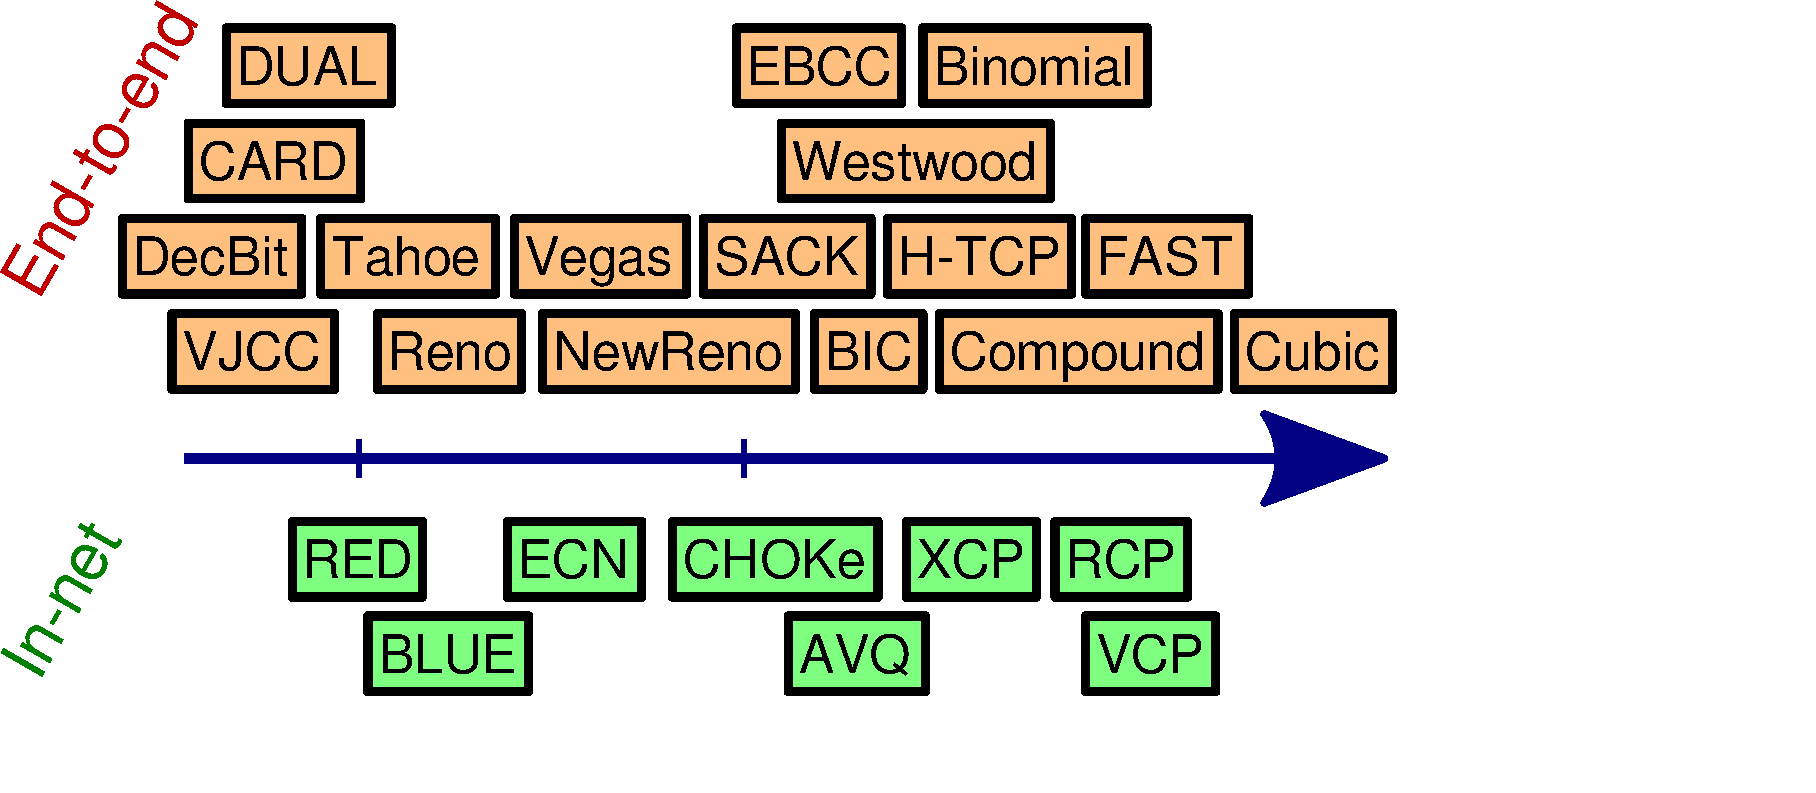
\includegraphics[width=1.1\textwidth]{march-2.pdf}

}
\only<4>{\noindent \hspace{-.75 cm} 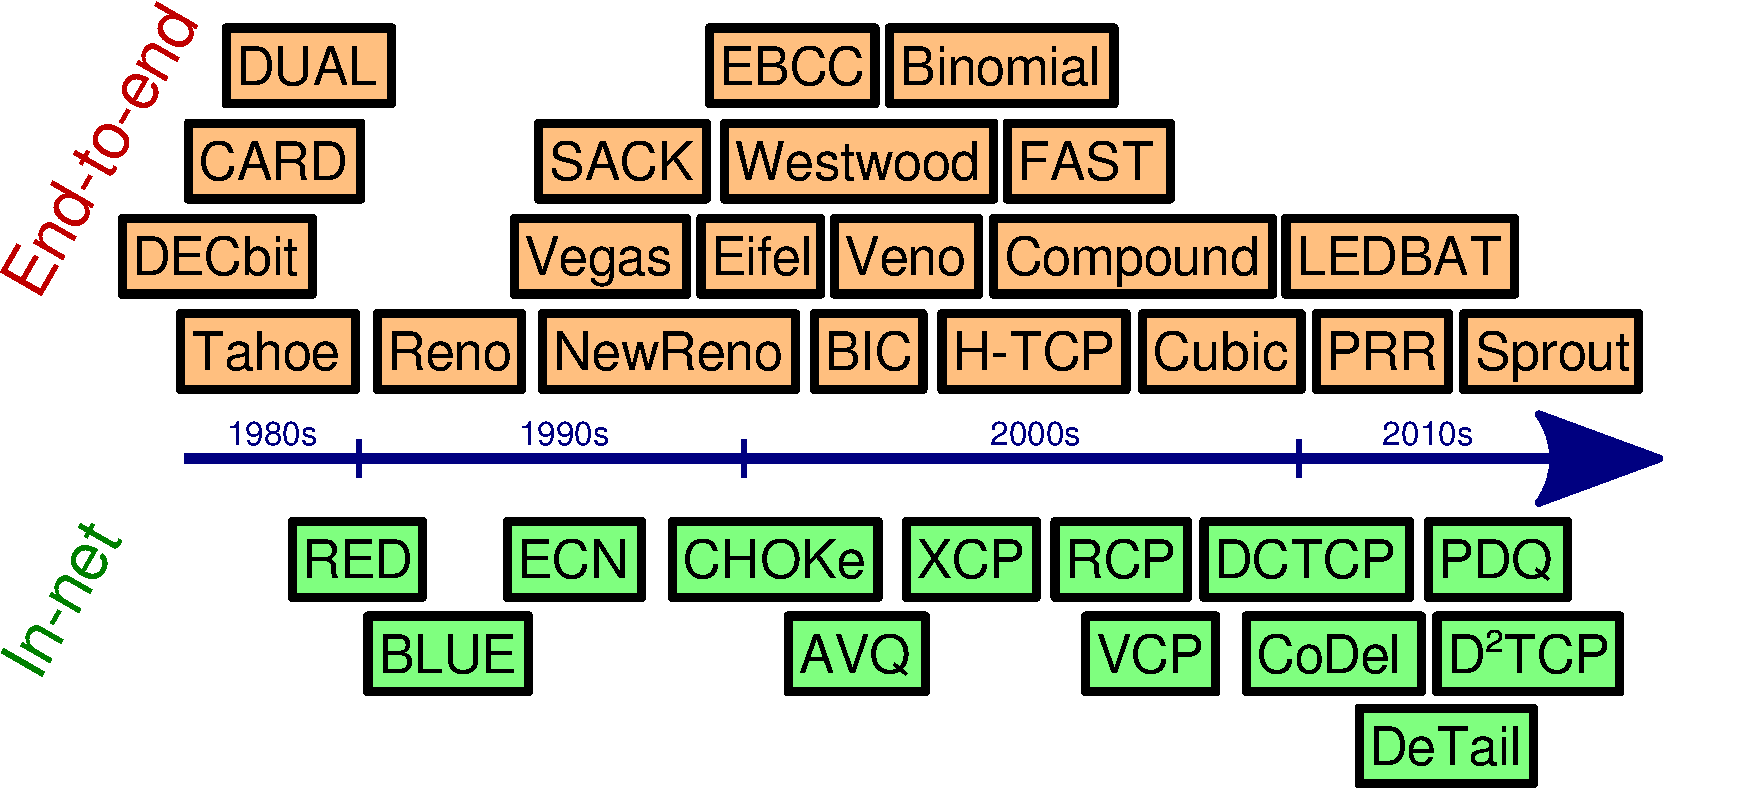
\includegraphics[width=1.1\textwidth]{march-1.pdf}

}
\only<5>{\noindent \hspace{-.75 cm} 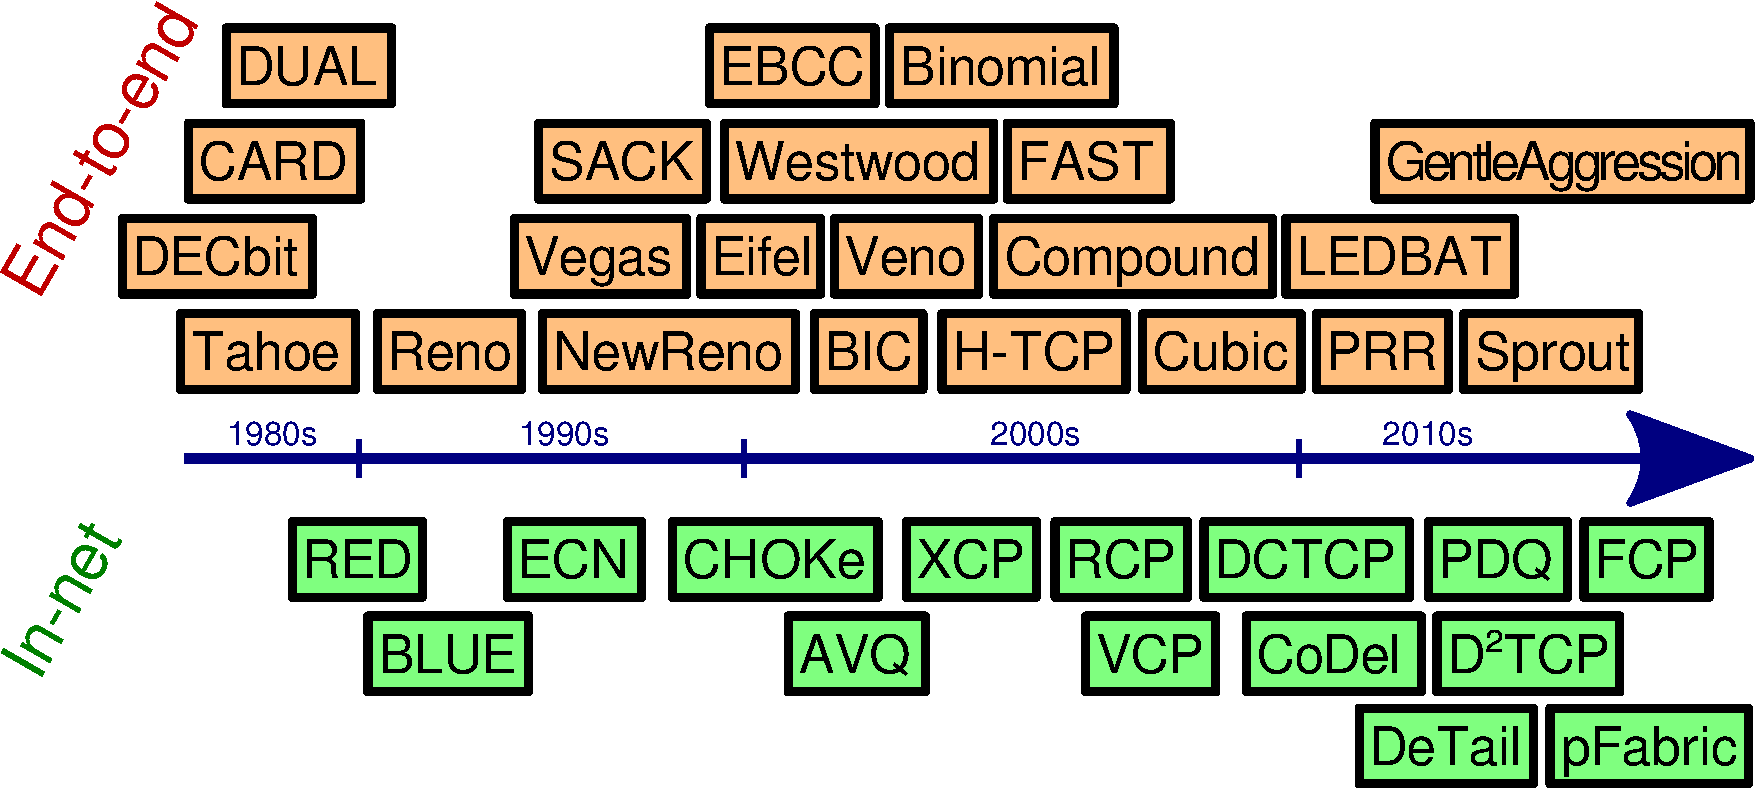
\includegraphics[width=1.1\textwidth]{march.pdf}

}
\end{frame}

%\begin{frame}
%\begin{centering}
%\LARGE One size does not fit all.
%
%\end{centering}
%\end{frame}

\begin{frame}

\frametitle{Our work}

\begin{centering}

\LARGE \textcolor{DarkGreen}{If congestion control is the answer,\\what's the question?}

\vspace{\baselineskip}

\pause

\LARGE \textcolor{NavyBlue}{Are there better answers?}

\end{centering}

\end{frame}

%\begin{frame}
%\frametitle{Rational choice of scheme is challenging}
%
%\begin{centering}
%
\includegraphics[height=20 pt]{cubic.pdf}\hspace{8 pt}{\bf vs.}\hspace{8 pt}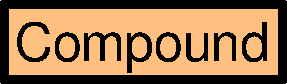
\includegraphics[height=20 pt]{compound.pdf}
%
%\end{centering}

%\ssline
%\ssline
%\ssline
%
%\begin{itemize}
%
%\Large
%
%\item Different goals?
%
%\item Different assumptions about network?
%
%\item One scheme just plain better?
%
%\end{itemize}
%
%\end{frame}

\begin{frame}
\frametitle{What are the ends that TCP tries to achieve?}

\begin{itemize}

\Large

\item ``Teleology of TCP'' is mostly unknown

\item Asymptotic solutions for long-running flows

\item Dynamical behavior is complex

\end{itemize}

\end{frame}

\begin{frame}
\frametitle{Networks constrained by a fuzzy idea of TCP's assumptions}

\Large

\begin{itemize}
\item Mask stochastic loss
\item Bufferbloat
\item Mask out-of-order delivery
\item No parallel/multipath routing
\item[]
\item[] {\it Advice for Internet Subnetwork Designers}\\ (RFC 3819) is 21,000 words!
\end{itemize}

\end{frame}

\begin{frame}
\frametitle{Apps hack around TCP}

\Large

\begin{itemize}
\item Open lots of flows \hspace{1.9 cm} \only<2->{
\includegraphics[width=0.5cm]{firefox.png} \hspace{0.001 cm} 
\includegraphics[width=0.5cm]{chrome-64.png} \hspace{0.001 cm} 
\includegraphics[width=0.5cm]{Internet_Explorer_10_logo.png} \hspace{0.02 cm} 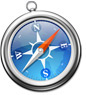
\includegraphics[width=0.5cm]{safari.jpg} \hspace{0.02 cm} 
\includegraphics[width=0.5cm]{mozilladino.png}}

\item Goose slow start \only<3->{\hspace{2.18 cm} \raisebox{-0.6ex}{
\includegraphics[height=14 pt]{Google_Logo_Old.PNG}} \raisebox{-.125 ex}{
\includegraphics[height=10 pt]{mslogo.png}}}

\item Add pacing \hspace{3.3 cm} \only<4->{\raisebox{-.4 ex}{
\includegraphics[height=14 pt]{youtube.png}}}

\item Give up and do it yourself

\visible<5>{
\small
\hspace{5.95 cm}\begin{minipage}{3.5 cm}
{\bf Chrome} \textcolor{DarkBlue}{(QUIC)} \\
{\bf BitTorrent} \textcolor{DarkBlue}{($\mu$TP)} \\
{\bf Mosh} \textcolor{DarkBlue}{(SSP)} \\
{\bf Aspera} \textcolor{DarkBlue}{(fasp)} \\
\end{minipage}
}

\end{itemize}

\end{frame}

\begin{frame}
\frametitle{Better: free the network to evolve}

\Large Transport layer should adapt to \textbf{\textcolor{DarkBlue}{whatever}}:

\begin{itemize}
\item network does

\item application wants

\end{itemize}

\end{frame}

\begin{frame}
\frametitle{What we built}

\colorbox{Bisque}{
\begin{centering}
\noindent \begin{tabular}{ll}
\Large \textcolor{DarkRed}{\bf Remy}: & \Large a program that generates \\ & \Large congestion-control schemes offline
\end{tabular}

\end{centering}}

\ssline
\ssline

\textcolor{DarkBlue}{\bf Input:}

\begin{itemize}
\item Prior assumptions \hspace{3.01 cm} \textcolor{DarkBlue}{(what network may do)}

\item Goal \hspace{5.275 cm}\textcolor{DarkBlue}{(what app wants)}
\end{itemize}

\textcolor{DarkBlue}{\bf Output:} CC algorithm for a TCP sender \hspace{0.177 cm}\textcolor{DarkBlue}{(RemyCC)}

\ssline

\textcolor{DarkBlue}{\bf Time:} a few hours

\ssline

\textcolor{DarkBlue}{\bf Cost:} \$5--\$10 on Amazon EC$^2$

\end{frame}

\begin{frame}
\frametitle{The basic question of congestion control}

\section{The problem}

\begin{centering}
\fbox{
\begin{minipage}{6 cm}
\LARGE At this moment, do I:

\begin{itemize}

\item send a packet
\item not send a packet?

\end{itemize}

\end{minipage}
}

\end{centering}

\end{frame}

\begin{frame}
\frametitle{Dumbbell network}

\only<1>{\noindent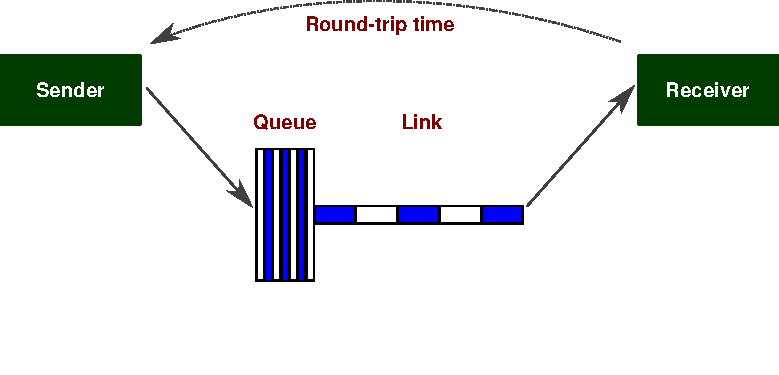
\includegraphics[width=\textwidth]{dumbbell-2.pdf}}\only<2>{\noindent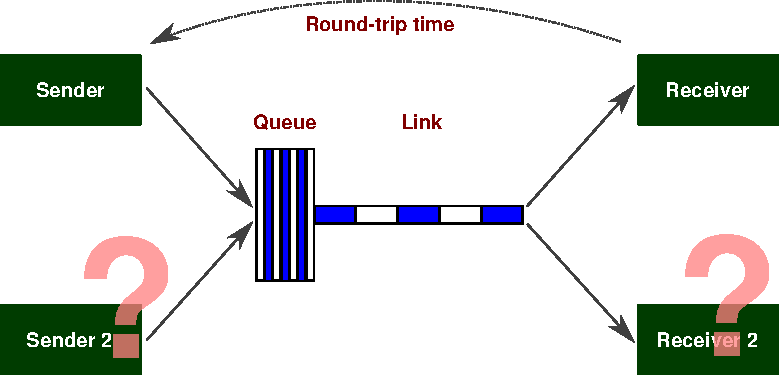
\includegraphics[width=\textwidth]{dumbbell-1.pdf}}\only<3>{\noindent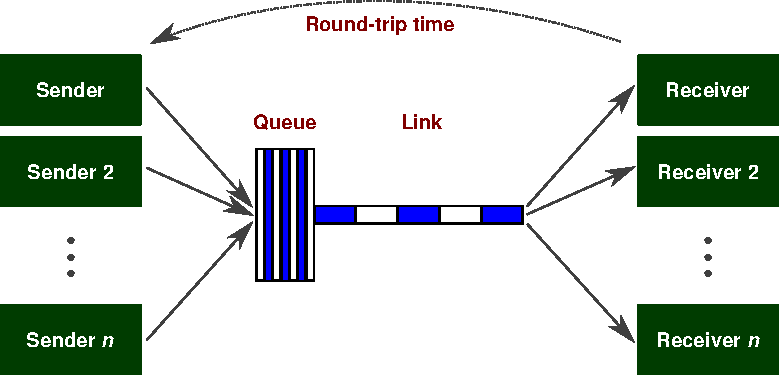
\includegraphics[width=\textwidth]{dumbbell.pdf}}

\end{frame}

%\begin{frame}
%\frametitle{The goal}
%
%\Large
%
%\begin{itemize}
%
%\item Tradeoff between \textbf{efficiency} and \textbf{fairness}
%
%\item Tradeoff between \textbf{throughput} and \textbf{delay}
%
%\end{itemize}
%
%\end{frame}

\begin{frame}
\frametitle{Objectives of congestion control}

\textbf{Minimize}

\begin{itemize}
\item average flow completion time

\item page load time

\item tail completion time

\end{itemize}

\textbf{Maximize}

\begin{itemize}

\item \begin{minipage}{3.75 cm}
$\min_i \textsf{throughput}_i$
\end{minipage} \textsf{\textcolor{DarkBlue}{(max-min throughput)}}

\item \begin{minipage}{3.75 cm}
\[\sum_i \log \left[ \textsf{throughput}_i \right]\]
\end{minipage} \textsf{\textcolor{DarkBlue}{(proportionally fair throughput)}}

\item
\begin{minipage}{3.75 cm}
\begin{tabular}{l}
\cellcolor{Bisque}\raisebox{0.75 cm}{\begin{minipage}{3.75 cm}
\[\sum_i \log \left[ \frac{\textsf{throughput}_i}{\visible<2>{
\textcolor{DarkBlue}{\big(}
}\textsf{delay}_i\visible<2>{
\textcolor{DarkBlue}{\big)^{\bm \delta}}}} \right]\]
\end{minipage} \textsf{\textcolor{DarkBlue}{(proportionally fair throughput/delay)}}}
\end{tabular}
\end{minipage}

\end{itemize}

\end{frame}

\begin{frame}
\frametitle{Prior knowledge}

\begin{itemize}

\Large

\item Model of network uncertainty

\begin{itemize}
\item Link speed distribution
\item Delay distribution
\end{itemize}

\item Traffic model

\begin{itemize}
\item Web browsing, MapReduce, videoconferencing
\end{itemize}

\item May be \textcolor{Red}{specific} or \textcolor{DarkBlue}{not very informative} \\

\vspace{4 pt}

\tiny \hspace{1.6 cm} \textcolor{Red}{(E.g., XCP, pFabric)} \hspace{0.2 cm} \textcolor{DarkBlue}{(Tahoe, Reno, Cubic)}
\end{itemize}

\end{frame}

\begin{frame}
\frametitle{Statement of the problem}

\Large

\begin{itemize}

\item Endpoints have no control over routing

\item Each sender only gets own receiver's acks

\item Goal: \textbf{\textcolor{DarkBlue}{optimize expected value of objective}}

%\item[] \normalsize $\Rightarrow$ decentralized partially-observable Markov decision process

\end{itemize}

\end{frame}

\begin{frame}
\frametitle{The intractable question of congestion control}

\begin{centering}
\fbox{
\begin{minipage}{6 cm}
\LARGE At this moment,\textcolor{DarkBlue}{\bf *} do I:

\begin{itemize}

\item send a packet
\item not send a packet?

\end{itemize}

\end{minipage}
}

\ssline
\ssline
\ssline

\pause

\end{centering}

\Large \noindent \hspace{-.5cm} \mbox{\textcolor{DarkBlue}{\textbf{*} Given {\bf full history} of packets sent and acks received!}}

\end{frame}

\begin{frame}
\frametitle{Remy: tractable search for the best}

\section{Remy}

\large

\begin{itemize}

\item Remy searches for the best congestion-control algorithm

\begin{itemize}
\item optimizes given objective over prior assumptions about network
\end{itemize}

\item \textbf{\textcolor{DarkBlue}{Approximates}} solution by limiting available state

\end{itemize}

\end{frame}

\begin{frame}
\frametitle{A RemyCC tracks three congestion signals}

\Large

\noindent \hspace{-0.75 cm}\begin{tabular}{ll}
\textcolor{DarkBlue}{$r\_ewma$}: & moving average of interval between acks \\

\textcolor{DarkBlue}{$s\_ewma$}: & \ldots between sender timestamps echoed in acks \\

\textcolor{DarkBlue}{$rtt\_ratio$}: & ratio of last RTT to smallest RTT so far \\

\end{tabular}

\end{frame}

\begin{frame}
\frametitle{Why these three congestion signals?}

\Large

\begin{itemize}

\item Benefit can be measured empirically

\begin{itemize}
\item In our experiments, little help from adding more
\item Other networks might find differently
\end{itemize}

\item More signals increase search time

\end{itemize}

\end{frame}

\begin{frame}
\frametitle{A RemyCC maps each state to an action}

\Large

\[\textsc{Rule}( \textcolor{DarkBlue}{r\_ewma}, \textcolor{DarkBlue}{s\_ewma}, \textcolor{DarkBlue}{rtt\_ratio} ) \rightarrow \langle \textcolor{Red}{m}, \textcolor{Red}{b}, \textcolor{Red}{r} \rangle \]

\ssline
\ssline

\begin{tabular}{ll}

\textcolor{Red}{$m$} & Multiple to congestion window \\

\textcolor{Red}{$b$} & Increment to congestion window \\

\textcolor{Red}{$r$} & Minimum interval between two outgoing packets \\

\end{tabular}

\end{frame}

\begin{frame}
\frametitle{Runtime for a RemyCC}

\large

\textbf{On ack:}

\begin{itemize}
\item $\langle \textcolor{Red}{m}, \textcolor{Red}{b}, \textcolor{Red}{r}\rangle \leftarrow \textsc{Rule}( \textcolor{DarkBlue}{r\_ewma}, \textcolor{DarkBlue}{s\_ewma}, \textcolor{DarkBlue}{rtt\_ratio} )$

\item $\texttt{cwnd} \leftarrow \textcolor{Red}{m} \cdot \texttt{cwnd} + \textcolor{Red}{b}$
\end{itemize}

\textbf{Send packet if:}

\begin{itemize}
\item $\texttt{cwnd} > \texttt{FlightSize}$, and

\item last packet sent $> \textcolor{Red}{r}$ ago
\end{itemize}

\end{frame}

\begin{frame}
\frametitle{Remy's job}

\Large

\colorbox{Bisque}{
\begin{minipage}{\textwidth}
Find piecewise-continuous \textsc{Rule}() that optimizes \\ expected value of objective function.

\end{minipage}}

\end{frame}

\begin{frame}
\frametitle{Remy example: Simplified RemyCC}

\large

\textbf{On ack:}

\begin{itemize}
\item $\langle \textcolor{Red}{m}, \textcolor{Red}{b}, \textcolor{Red}{r}\rangle \leftarrow \textsc{Rule}( r\_ewma, s\_ewma\visible<1>{, \textcolor{DarkBlue}{\textbf{rtt\_ratio}}}\visible<2>{} )$
\end{itemize}

\end{frame}

\begin{frame}
\frametitle{Remy example: Prior assumptions}

\large

\begin{tabular}{llll}
\bf Quantity & & \bf Distribution & \bf Units \\

\hline Link speed & & Uniform(10, 20) & Mbps \\

RTT & & Uniform(100, 200) & ms \\

$n$ & & Uniform(1, 16) \\

``On'' process & & $\mathrm{exp}[\mu = 5]$ & seconds \\

``Off'' process & & same \\

\end{tabular}

\end{frame}

\begin{frame}
\frametitle{Remy example: Objective}

\LARGE

\[\sum_i \log \left[ \frac{\textsf{throughput}_i}{\textsf{delay}_i} \right]\]

\end{frame}

\begin{frame}
\frametitle{Optimize default action}
\begin{centering}
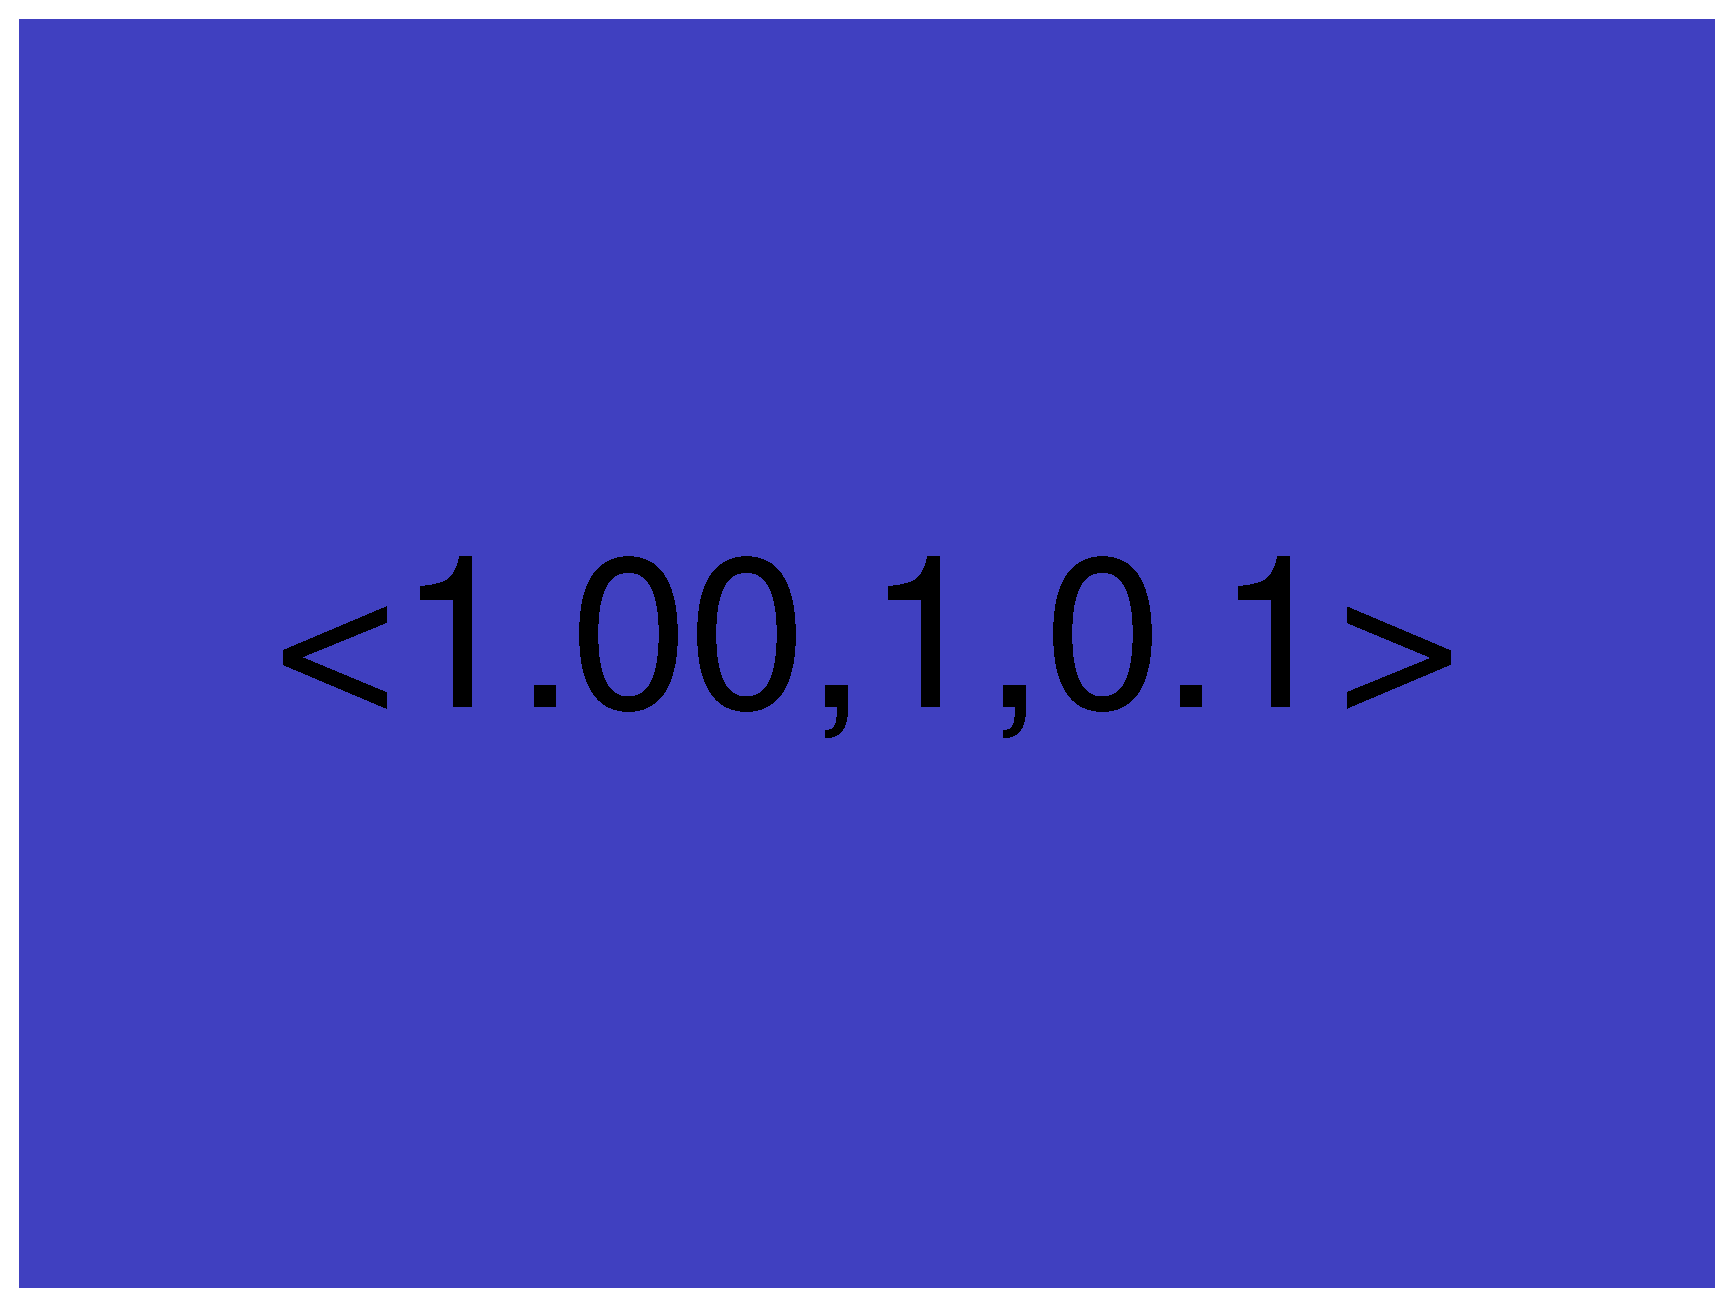
\includegraphics[width=8.5 cm]{remy-graph/graph/test0.pdf}

\end{centering}
\end{frame}

\begin{frame}
\frametitle{Split and duplicate at median query}
\begin{centering}
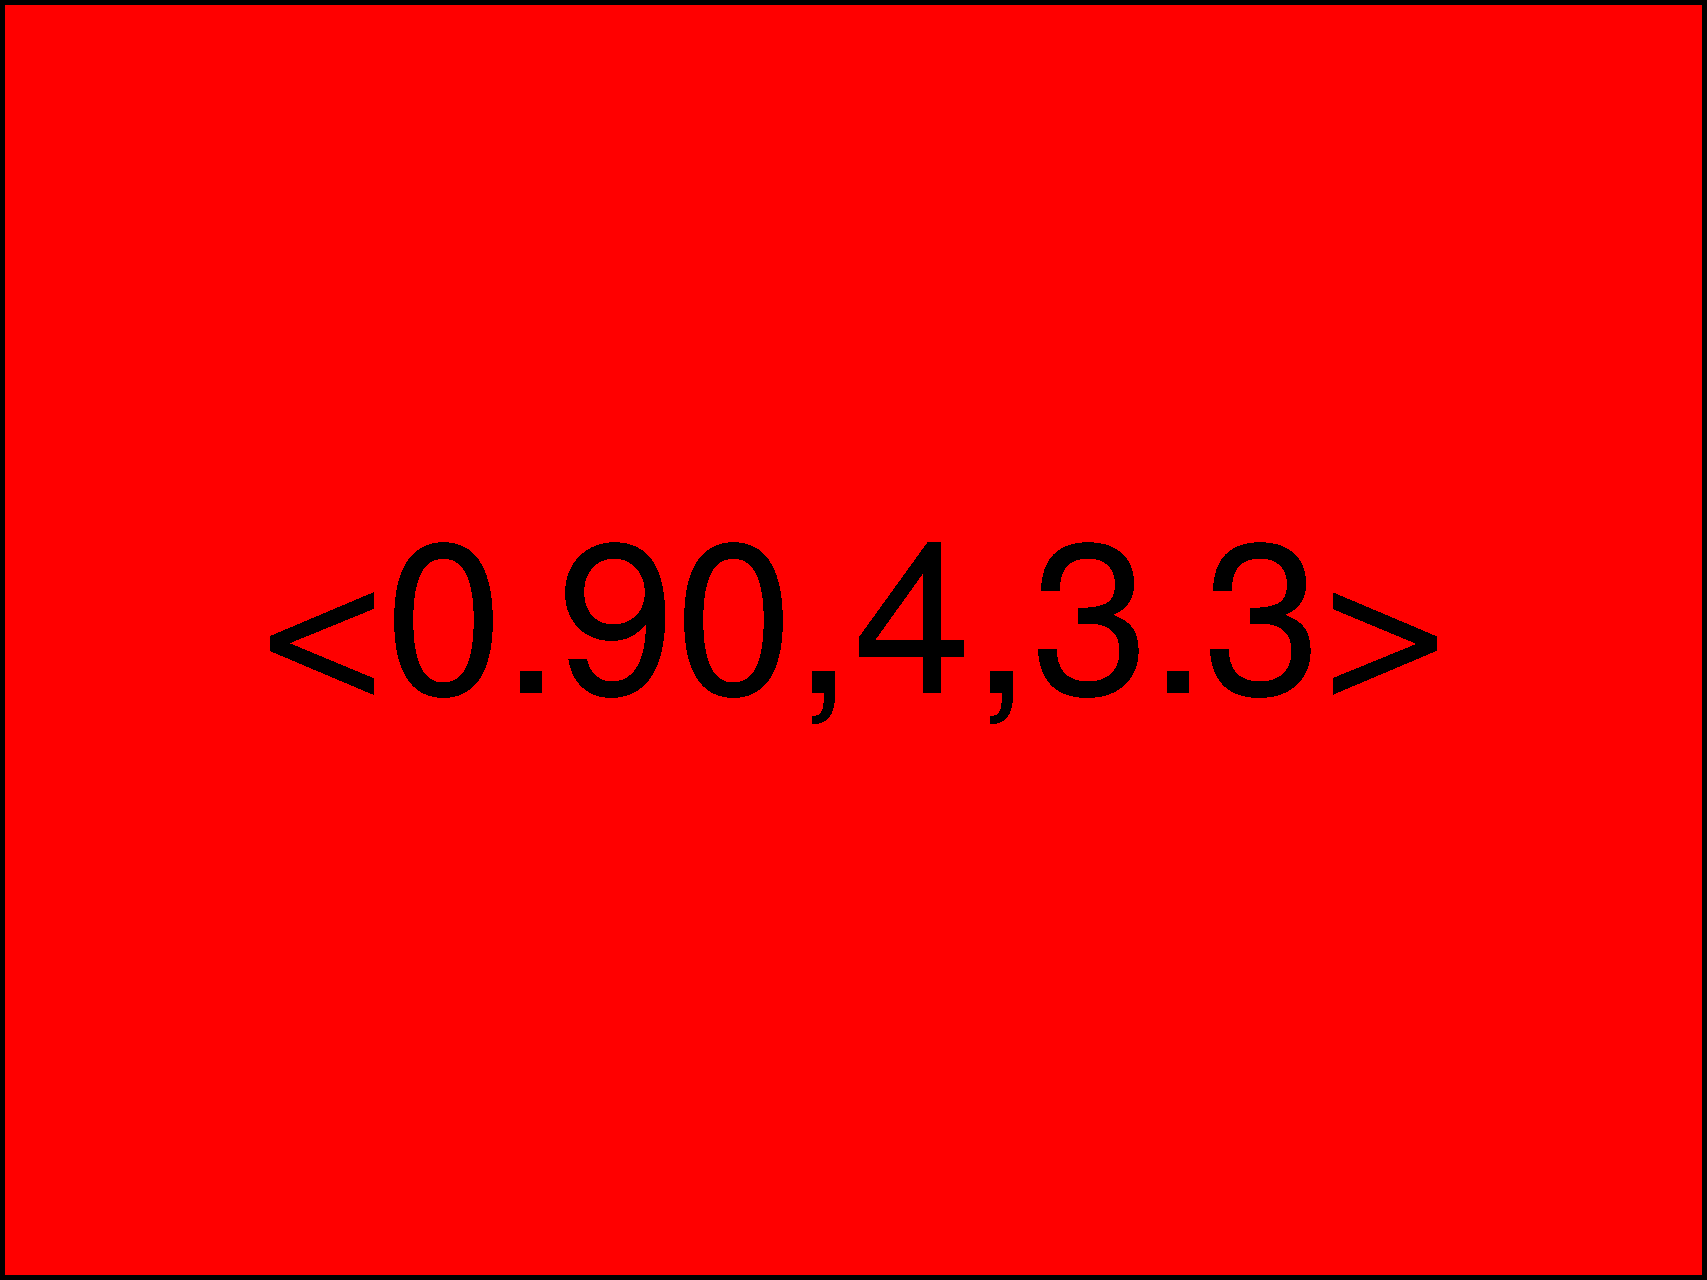
\includegraphics[width=8.5 cm]{remy-graph/graph/test1.pdf}

\end{centering}
\end{frame}

\begin{frame}
\frametitle{Run in simulation}
\begin{centering}
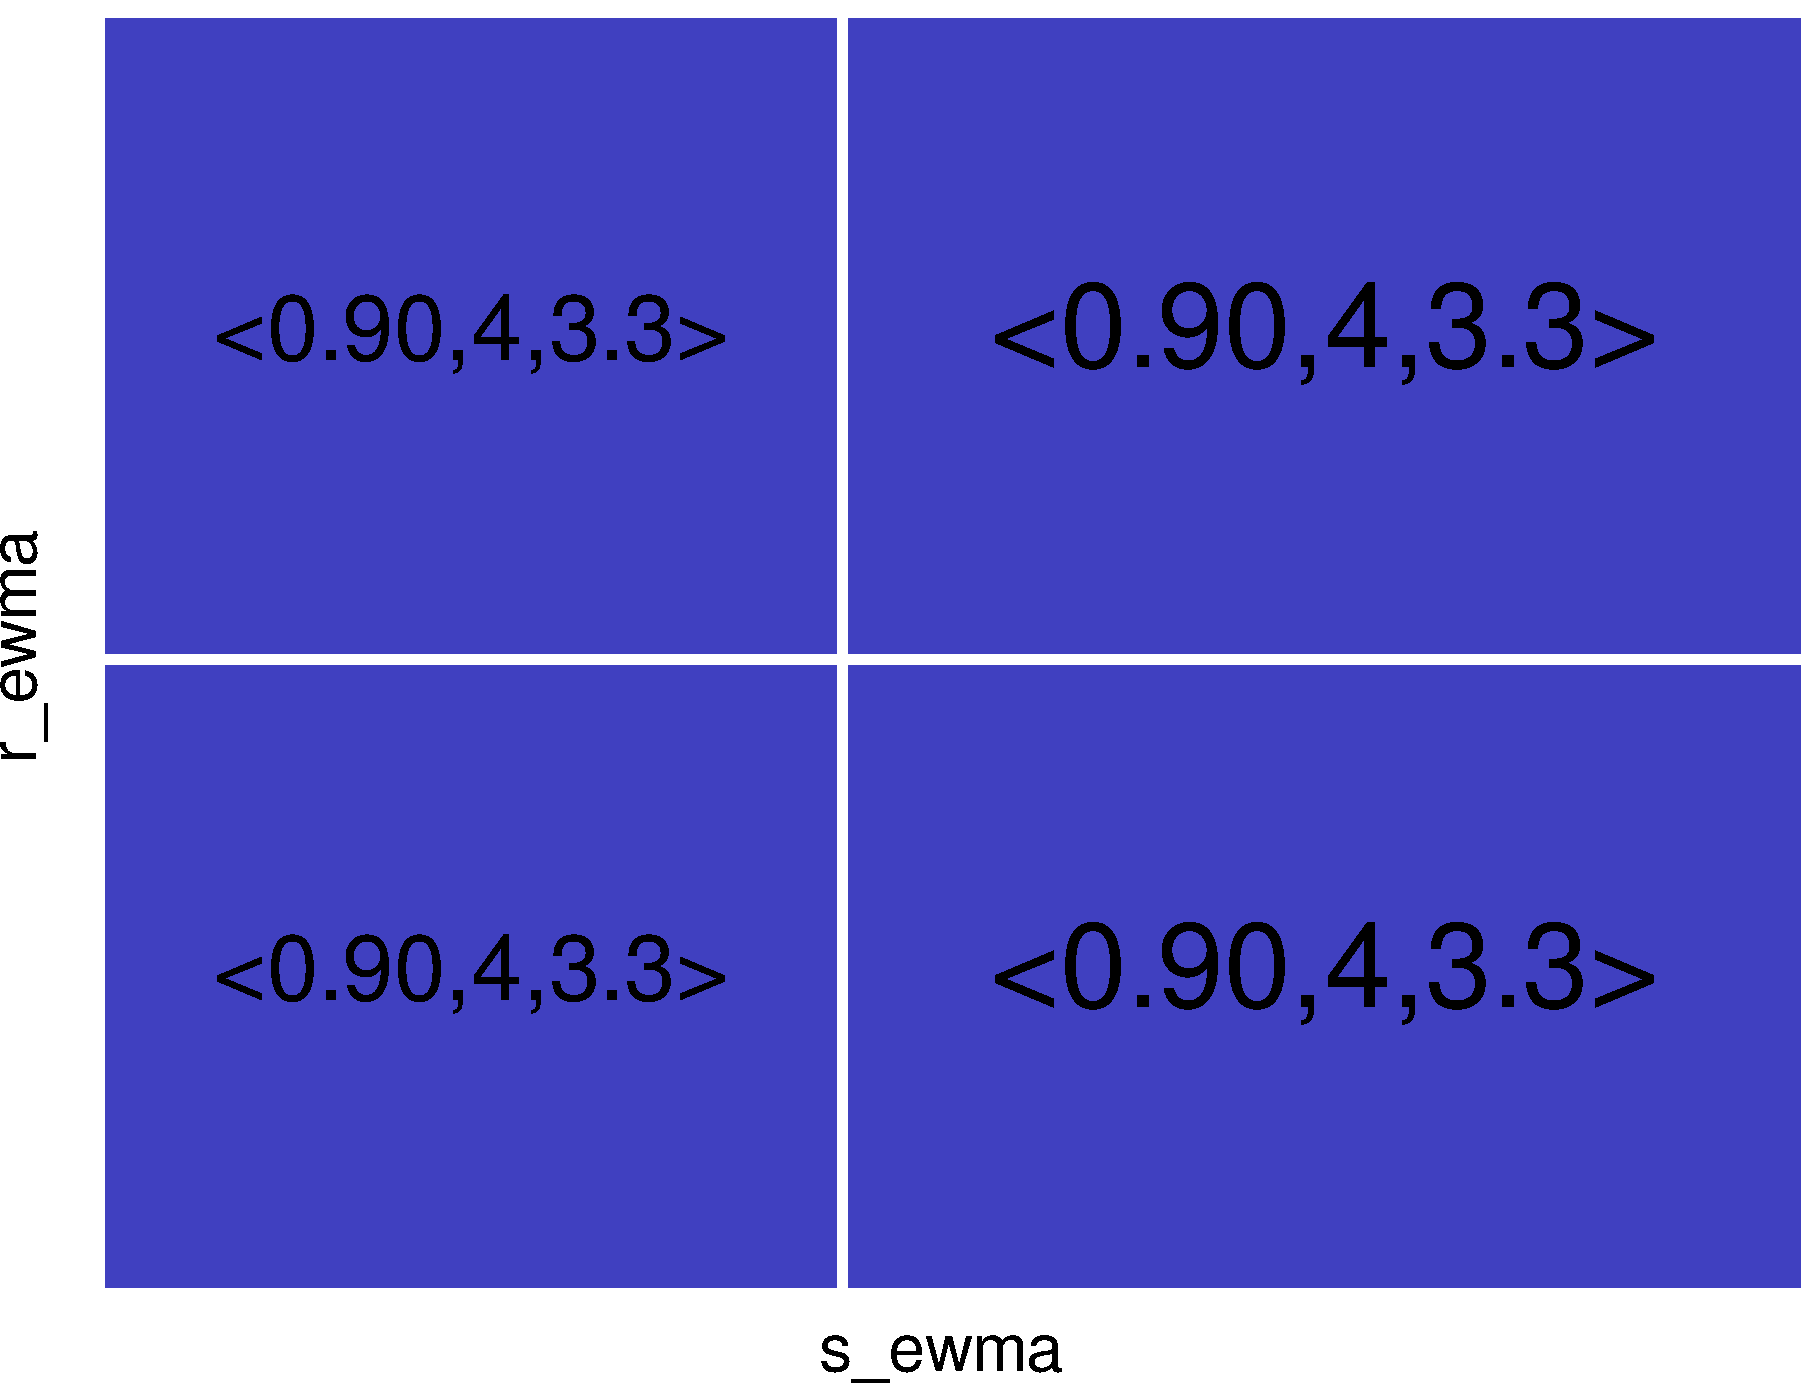
\includegraphics[width=8.5 cm]{remy-graph/graph/test2.pdf}

\end{centering}
\end{frame}

\begin{frame}
\frametitle{Optimize all actions}
\begin{centering}
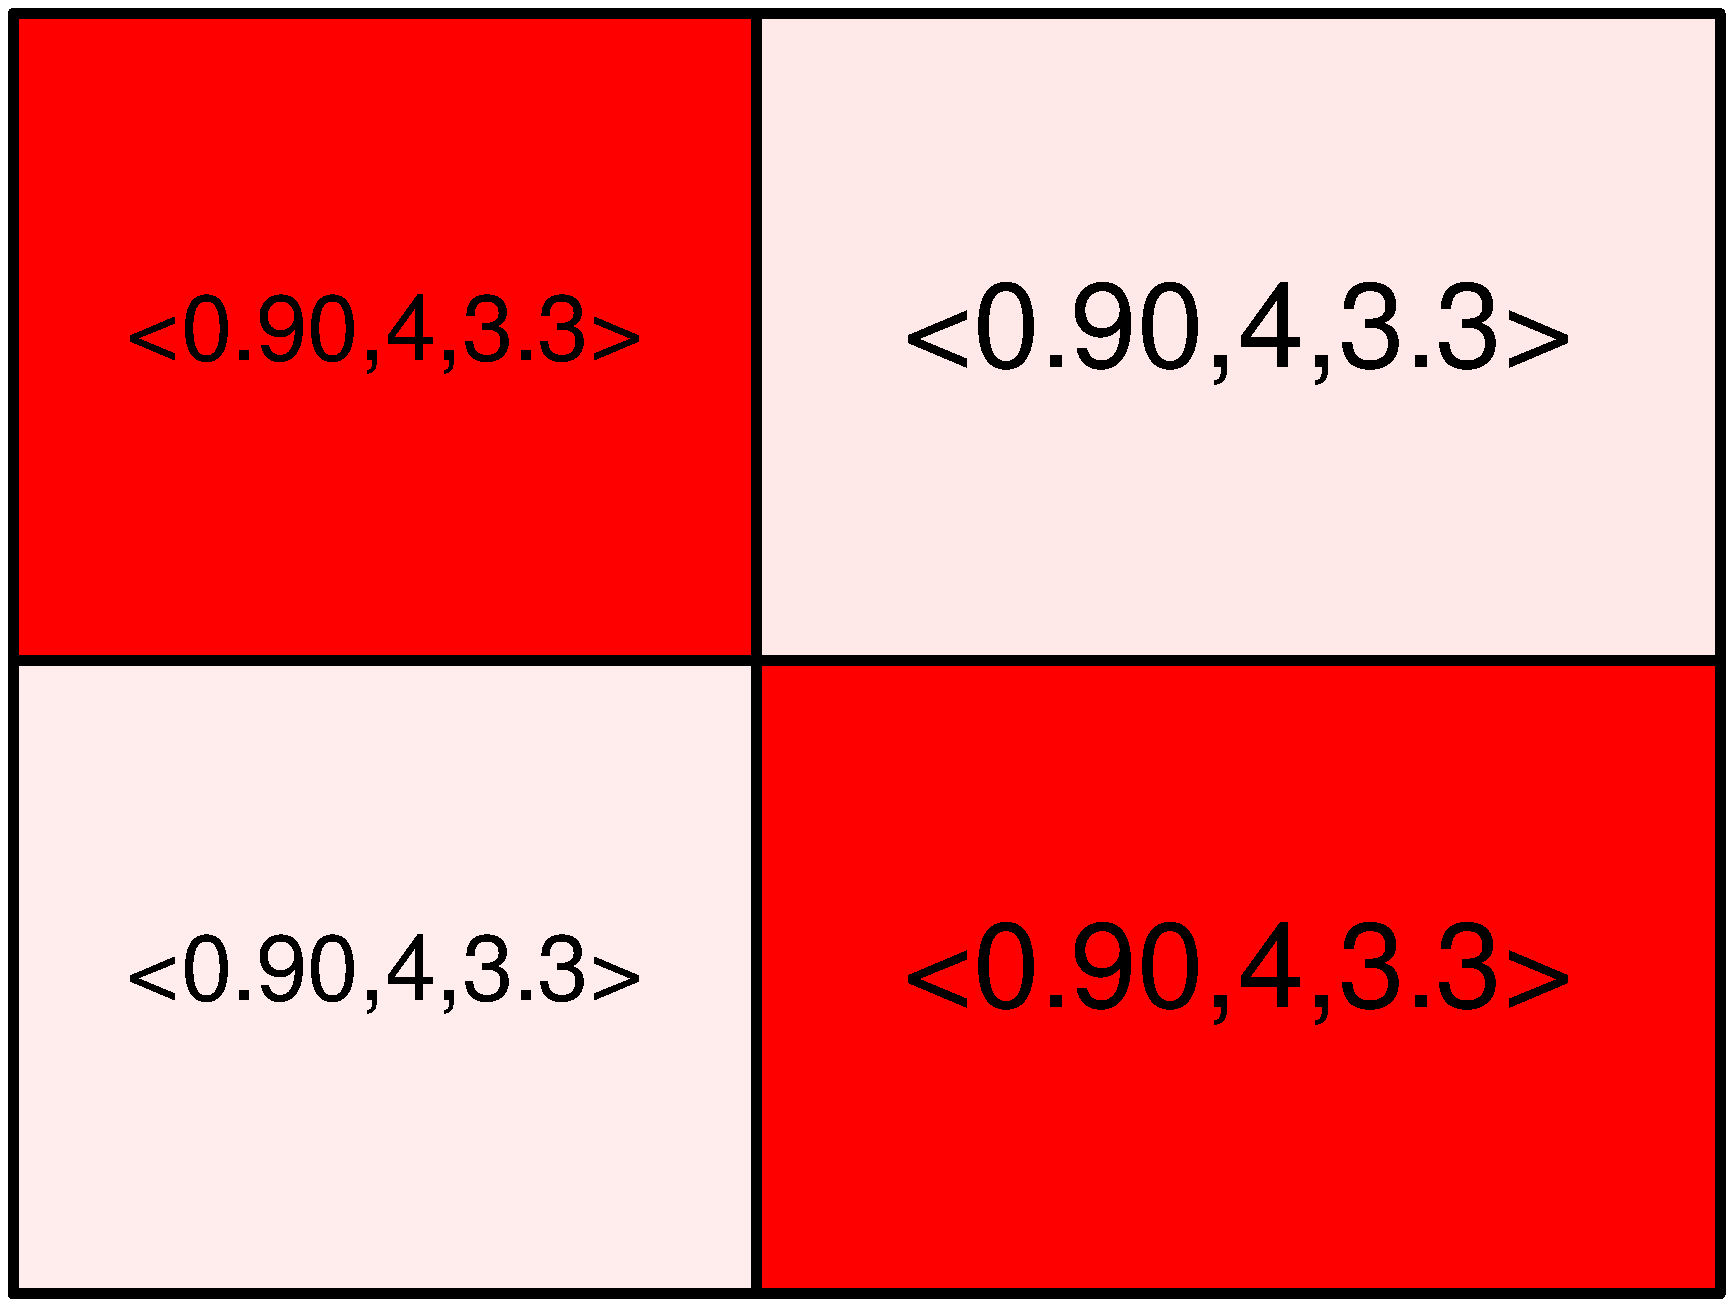
\includegraphics[width=8.5 cm]{remy-graph/graph/test3.pdf}

\end{centering}
\end{frame}

\begin{frame}
\frametitle{Split most-used rule}
\begin{centering}
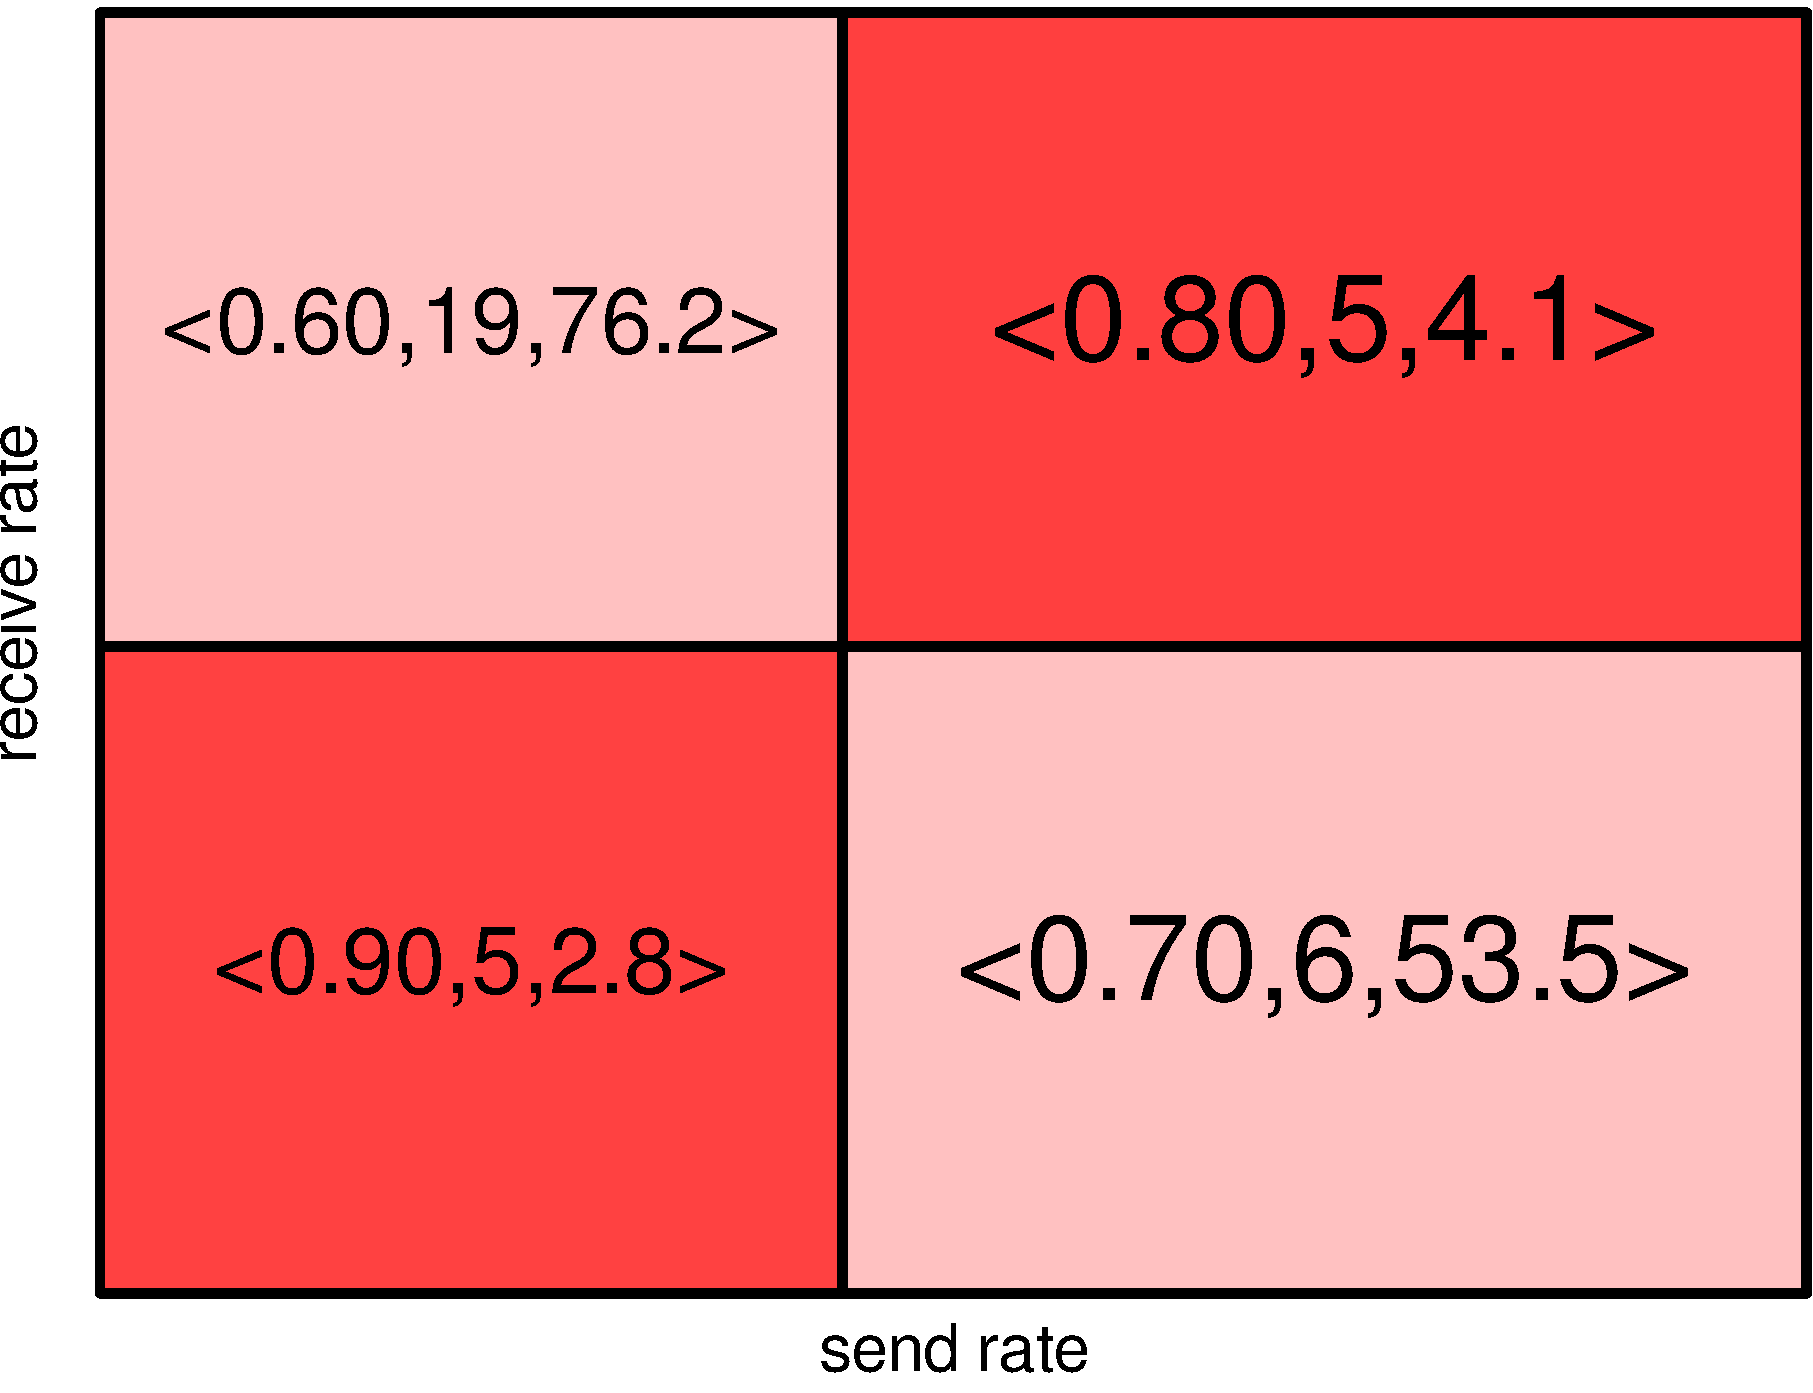
\includegraphics[width=8.5 cm]{remy-graph/graph/test4.pdf}

\end{centering}
\end{frame}

\begin{frame}
\frametitle{Iterate}
\begin{centering}
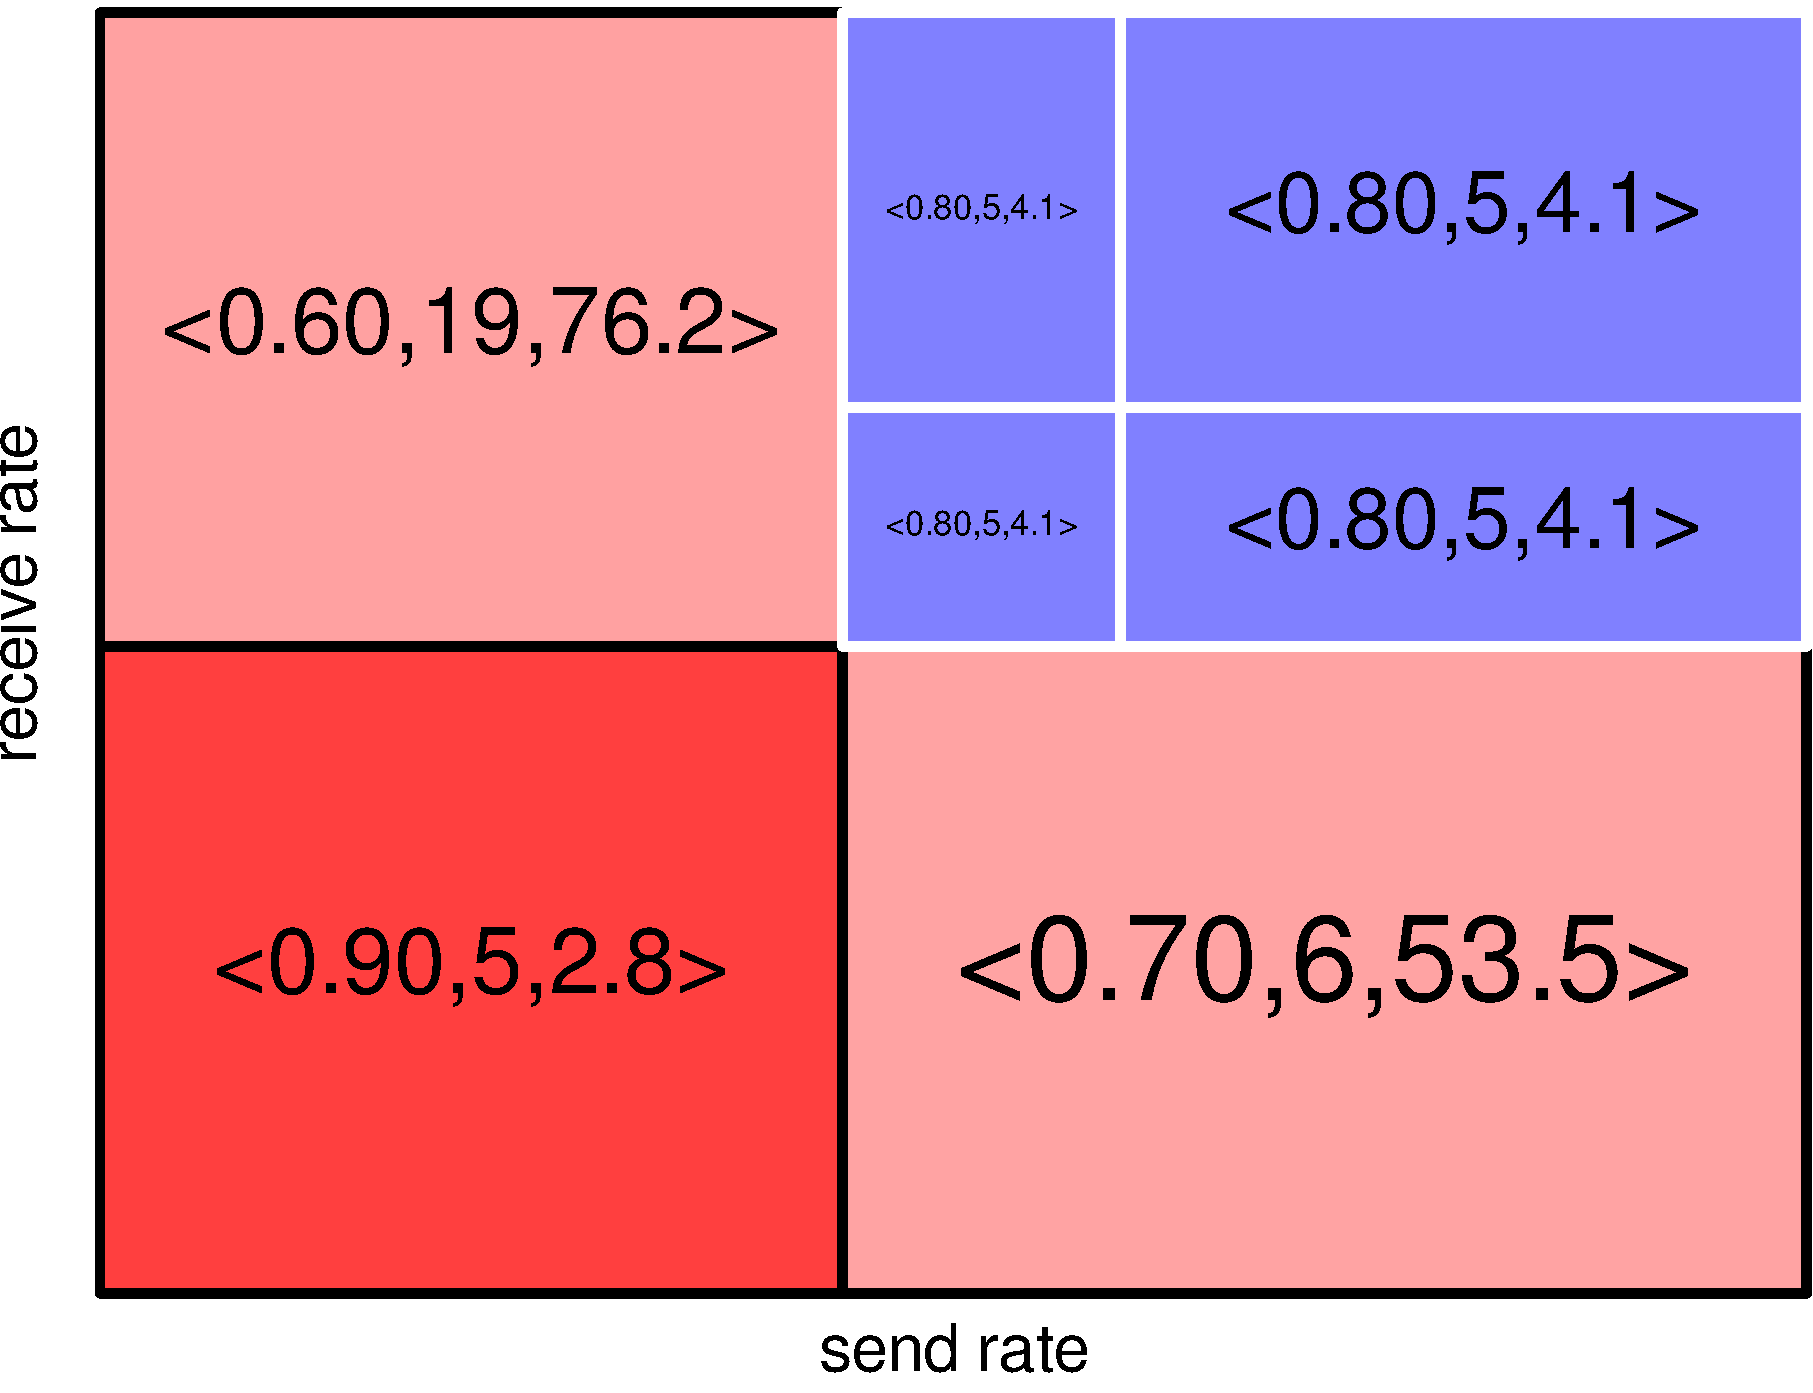
\includegraphics[width=8.5 cm]{remy-graph/graph/test5.pdf}

\end{centering}
\end{frame}

\begin{frame}
\frametitle{Iterate}
\begin{centering}
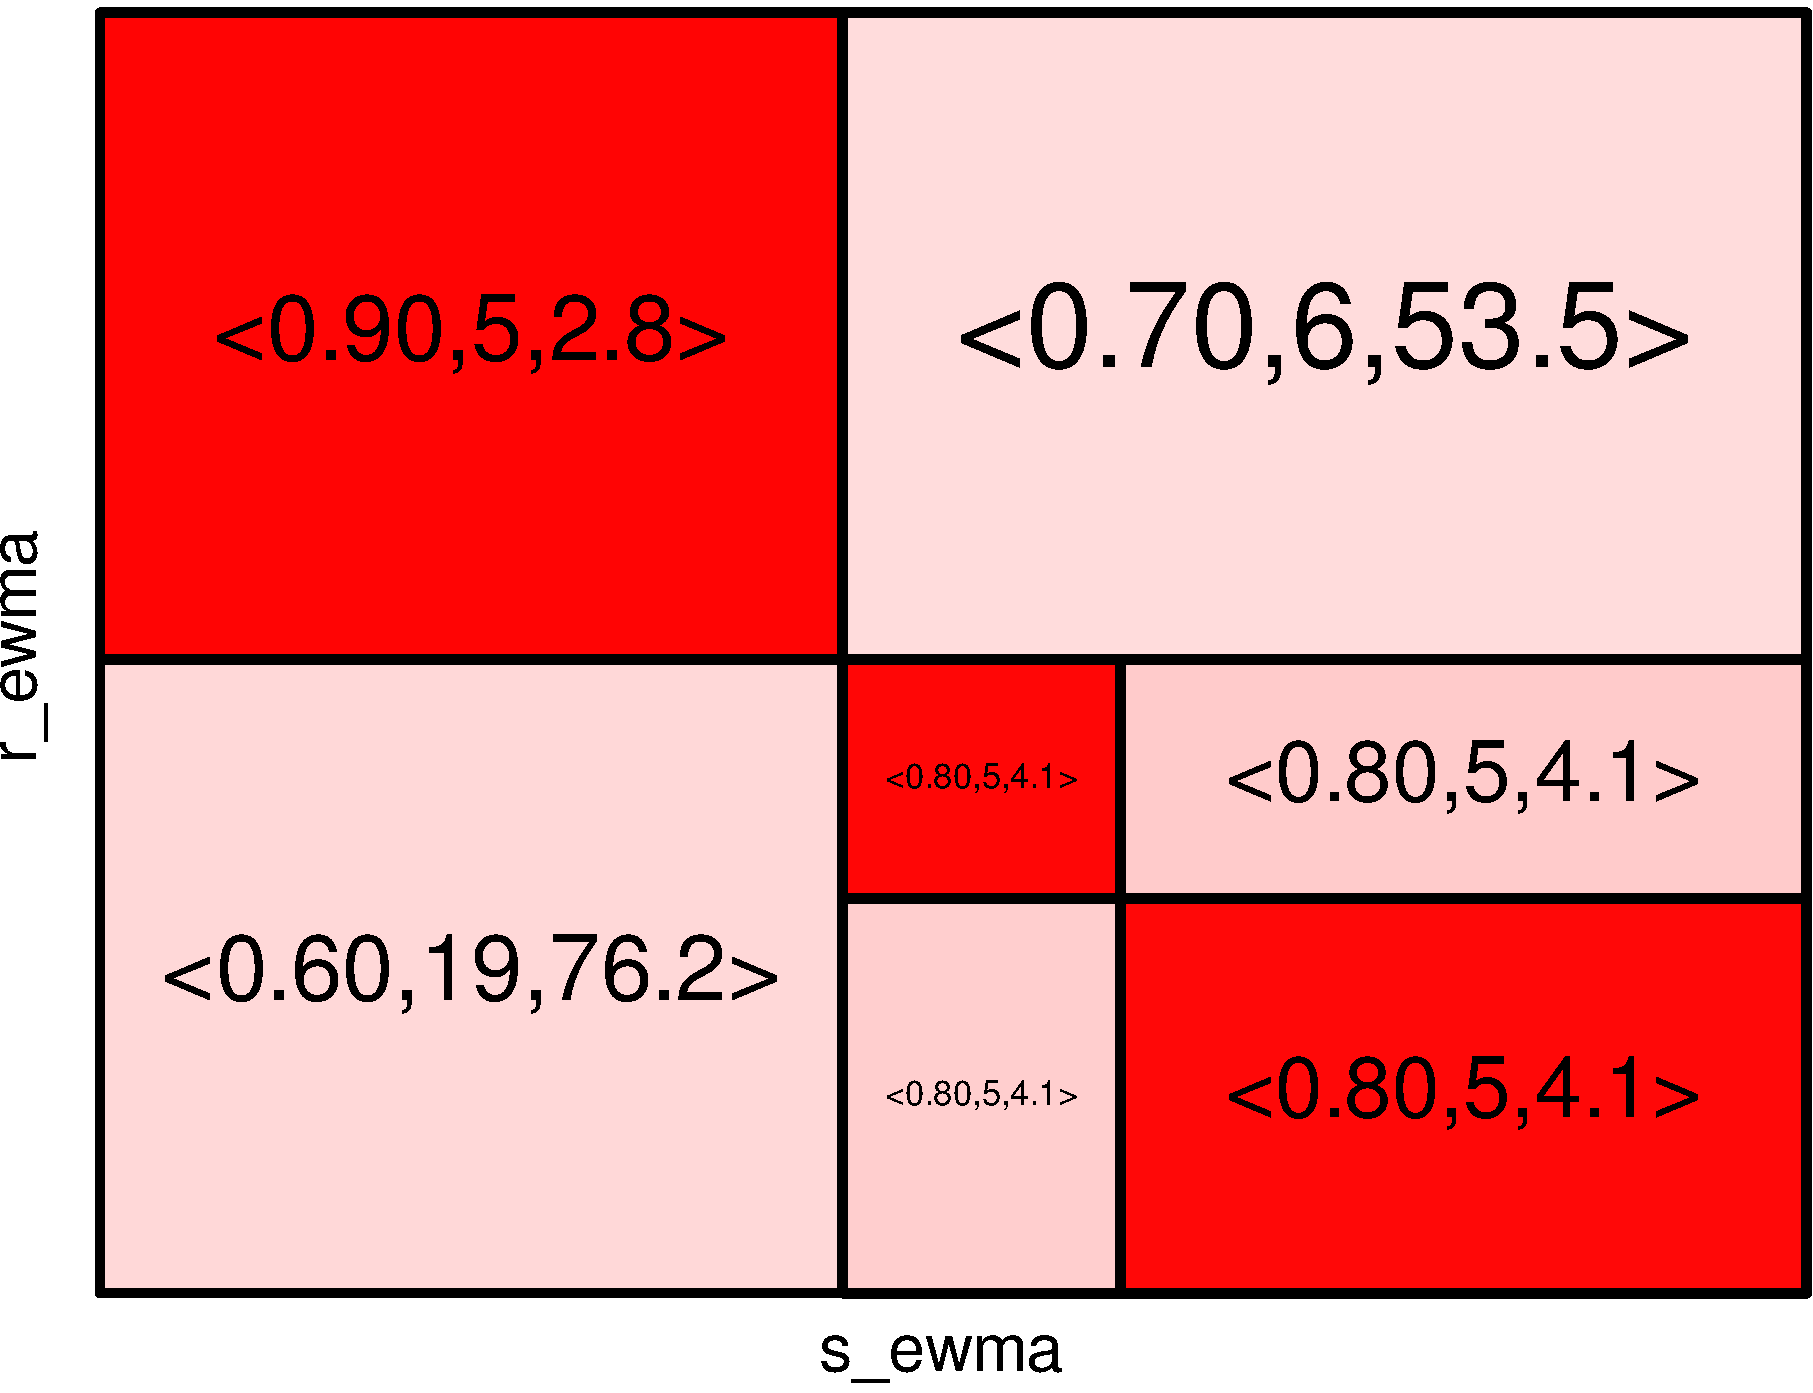
\includegraphics[width=8.5 cm]{remy-graph/graph/test6.pdf}

\end{centering}
\end{frame}
\begin{frame}
\frametitle{Iterate}\begin{centering}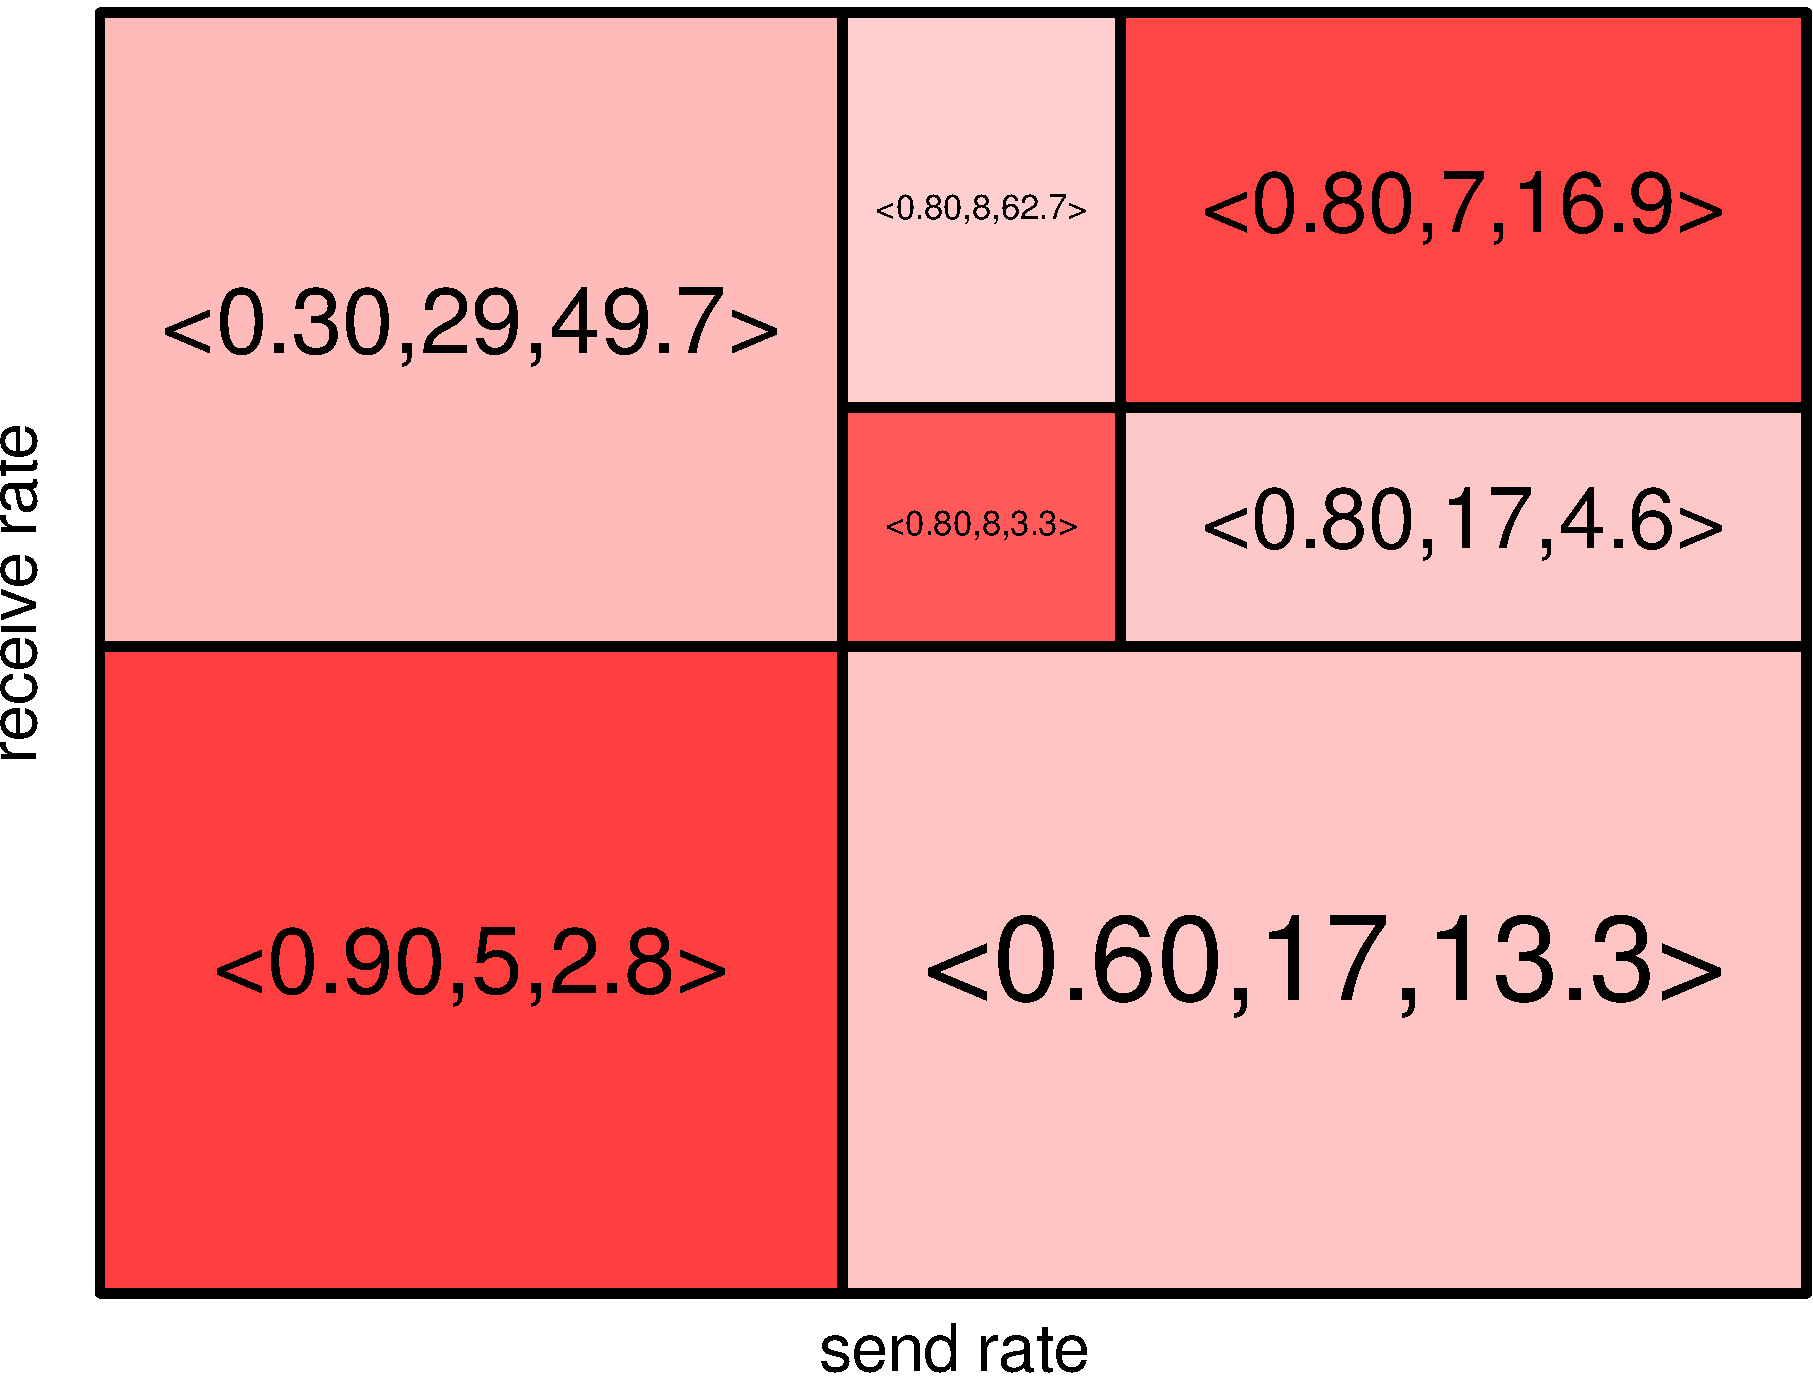
\includegraphics[width=8.5 cm]{remy-graph/graph/test7.pdf}

\end{centering}\end{frame}


\begin{frame}
\frametitle{Iterate}\begin{centering}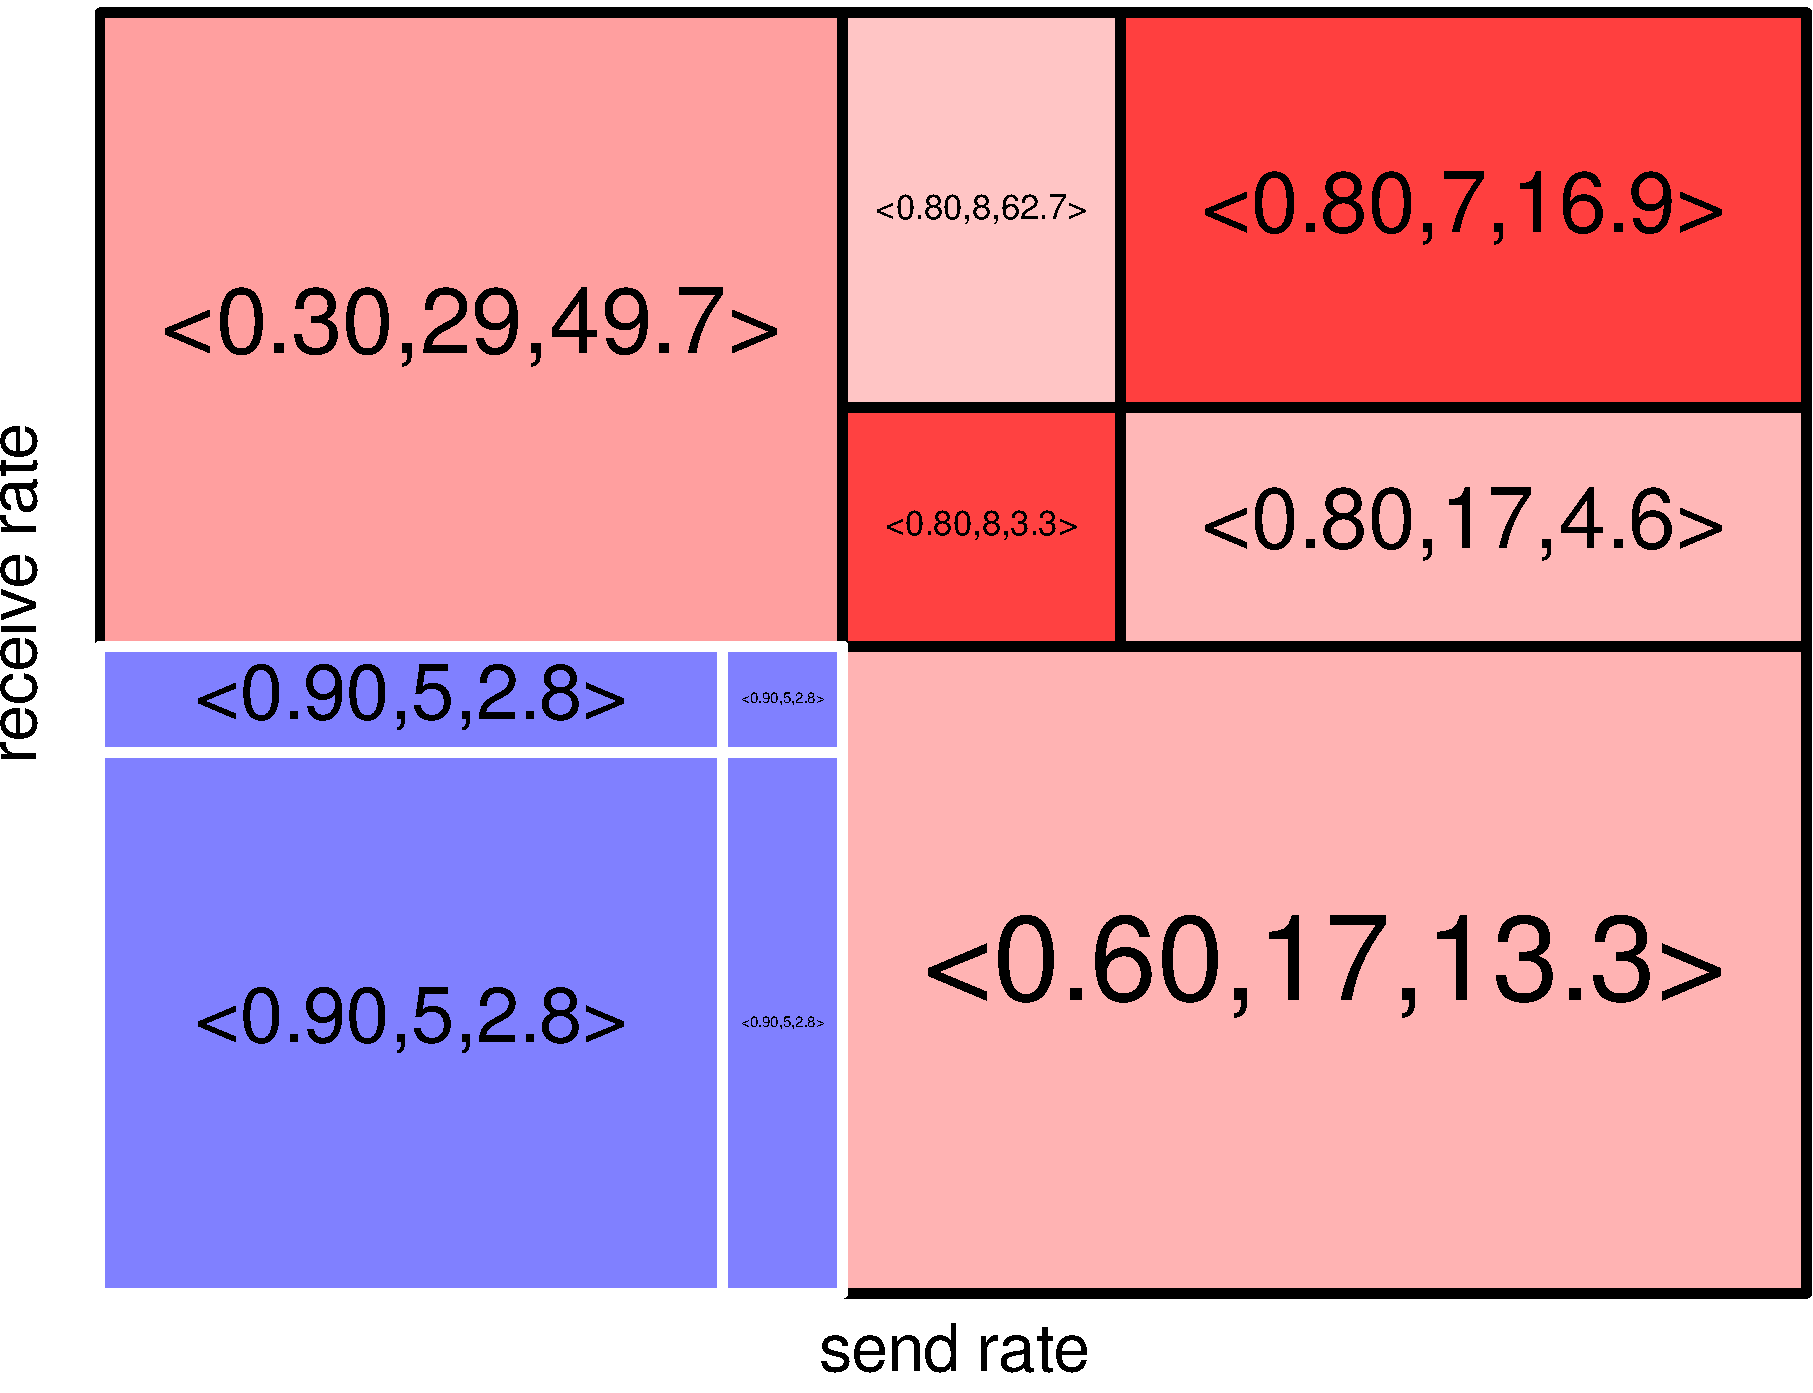
\includegraphics[width=8.5 cm]{remy-graph/graph/test8.pdf}

\end{centering}\end{frame}


\begin{frame}
\frametitle{Iterate}\begin{centering}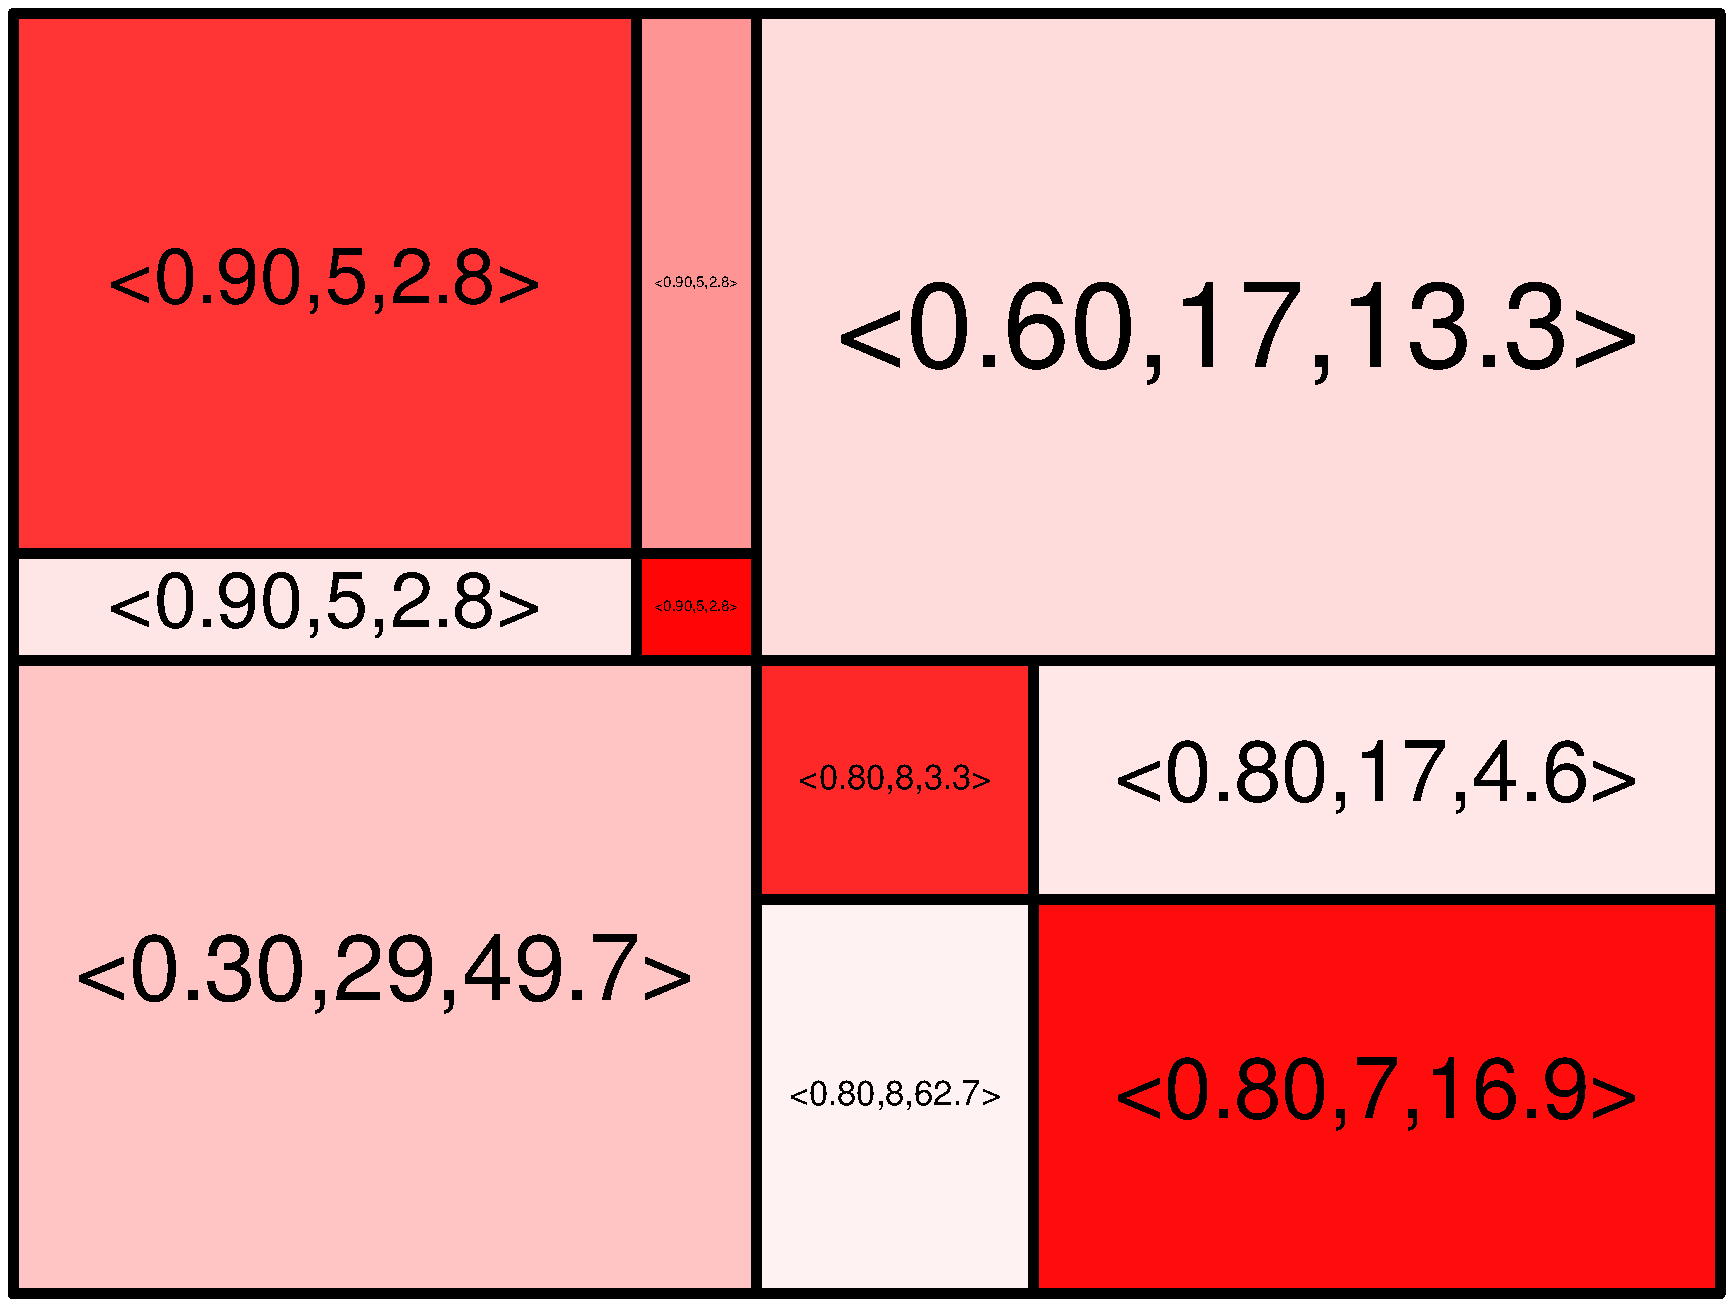
\includegraphics[width=8.5 cm]{remy-graph/graph/test9.pdf}

\end{centering}\end{frame}


\begin{frame}
\frametitle{Iterate}\begin{centering}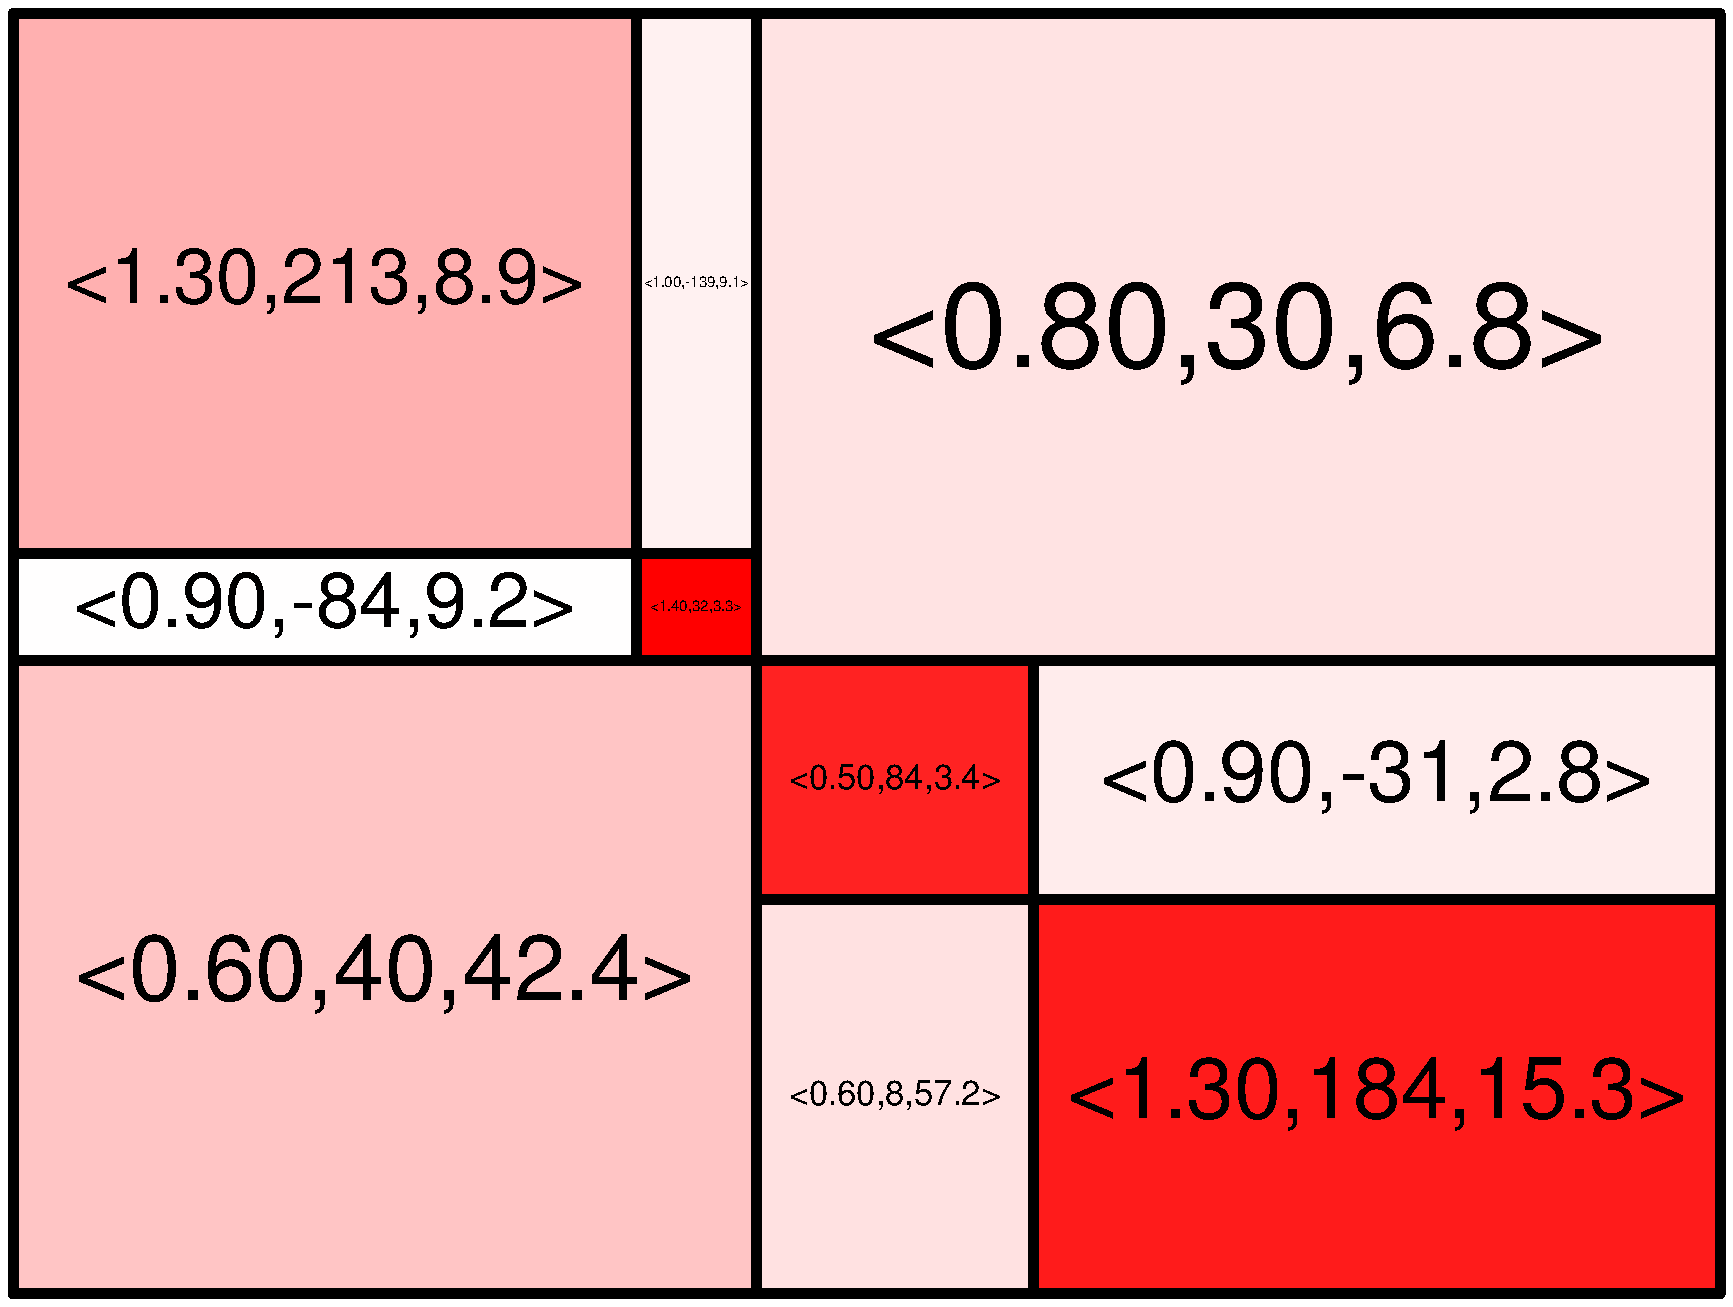
\includegraphics[width=8.5 cm]{remy-graph/graph/test10.pdf}

\end{centering}\end{frame}


\begin{frame}
\frametitle{Iterate}\begin{centering}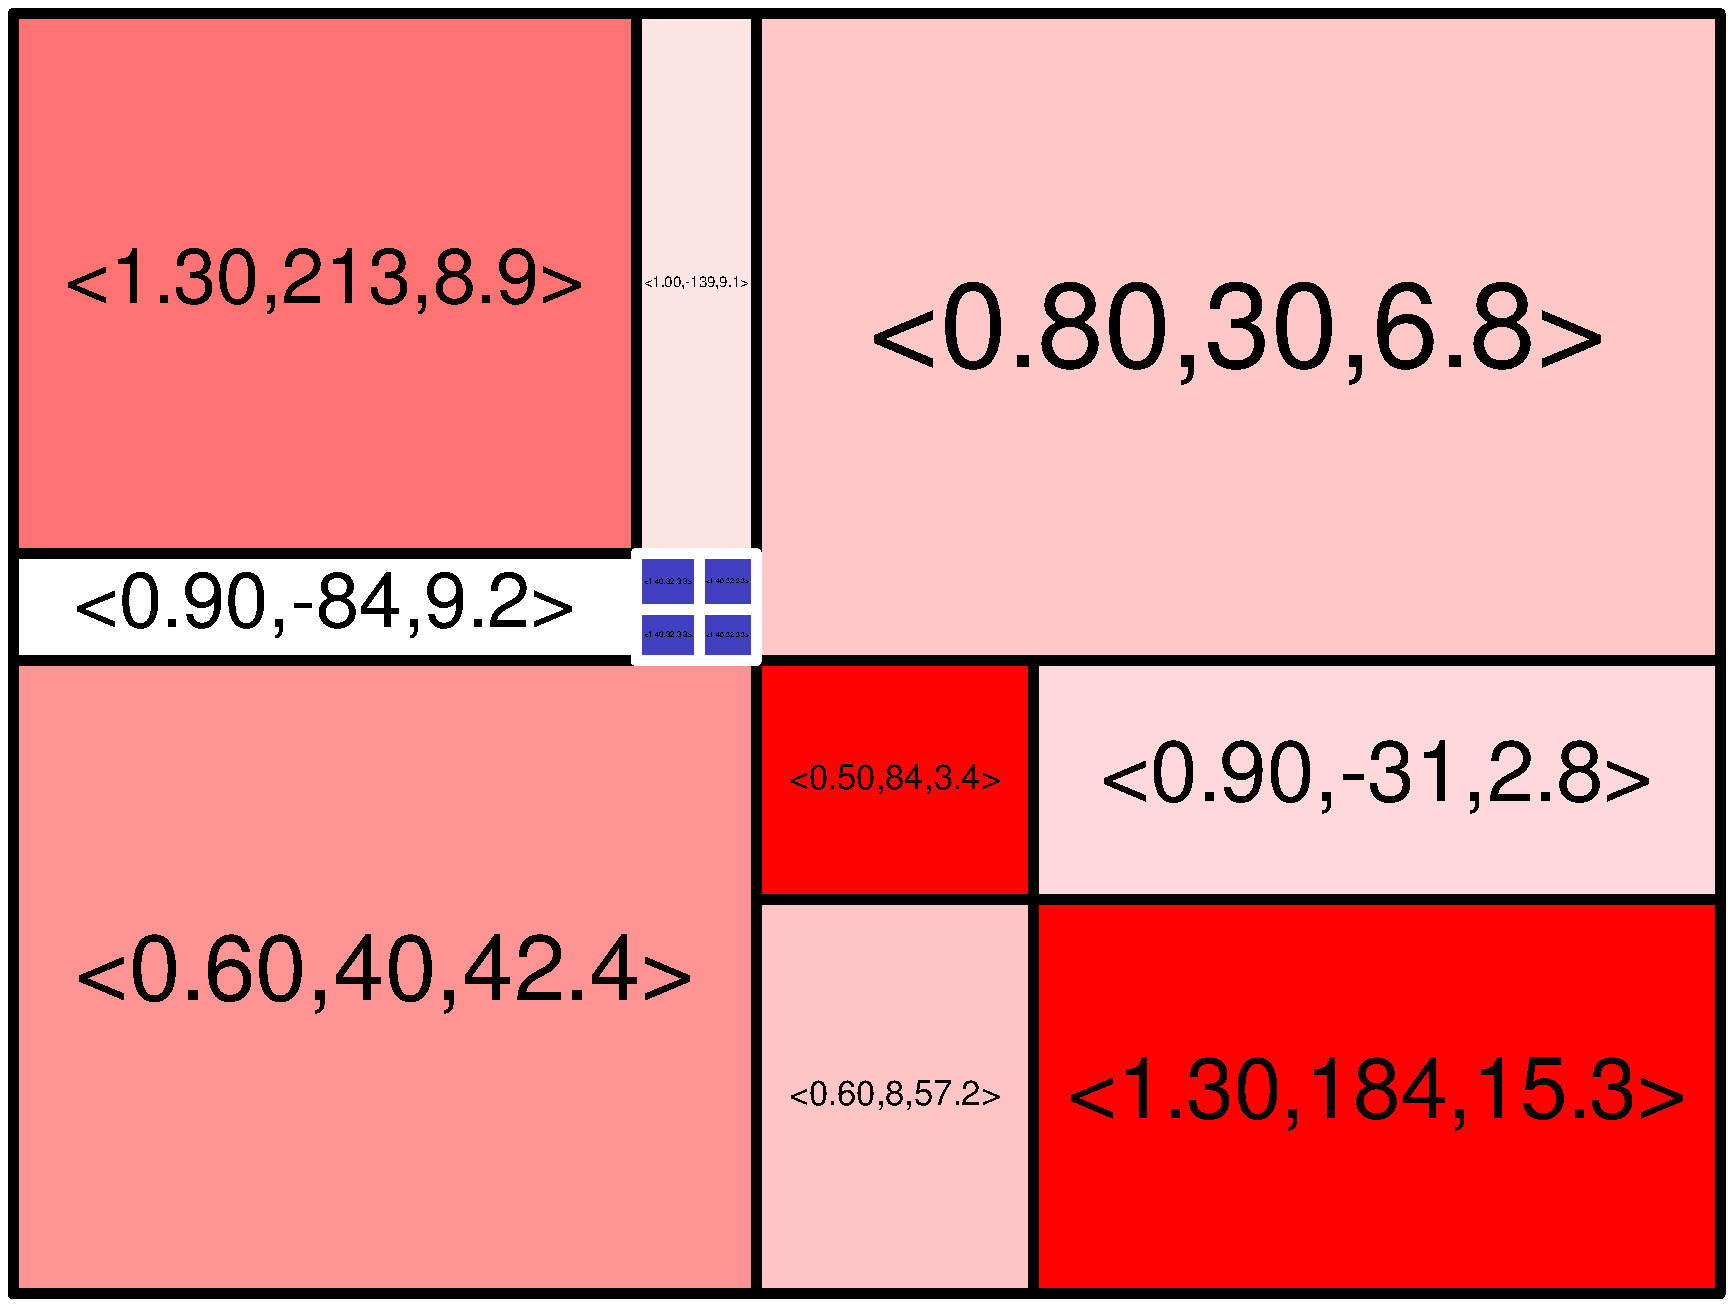
\includegraphics[width=8.5 cm]{remy-graph/graph/test11.pdf}

\end{centering}\end{frame}


\begin{frame}
\frametitle{Iterate}\begin{centering}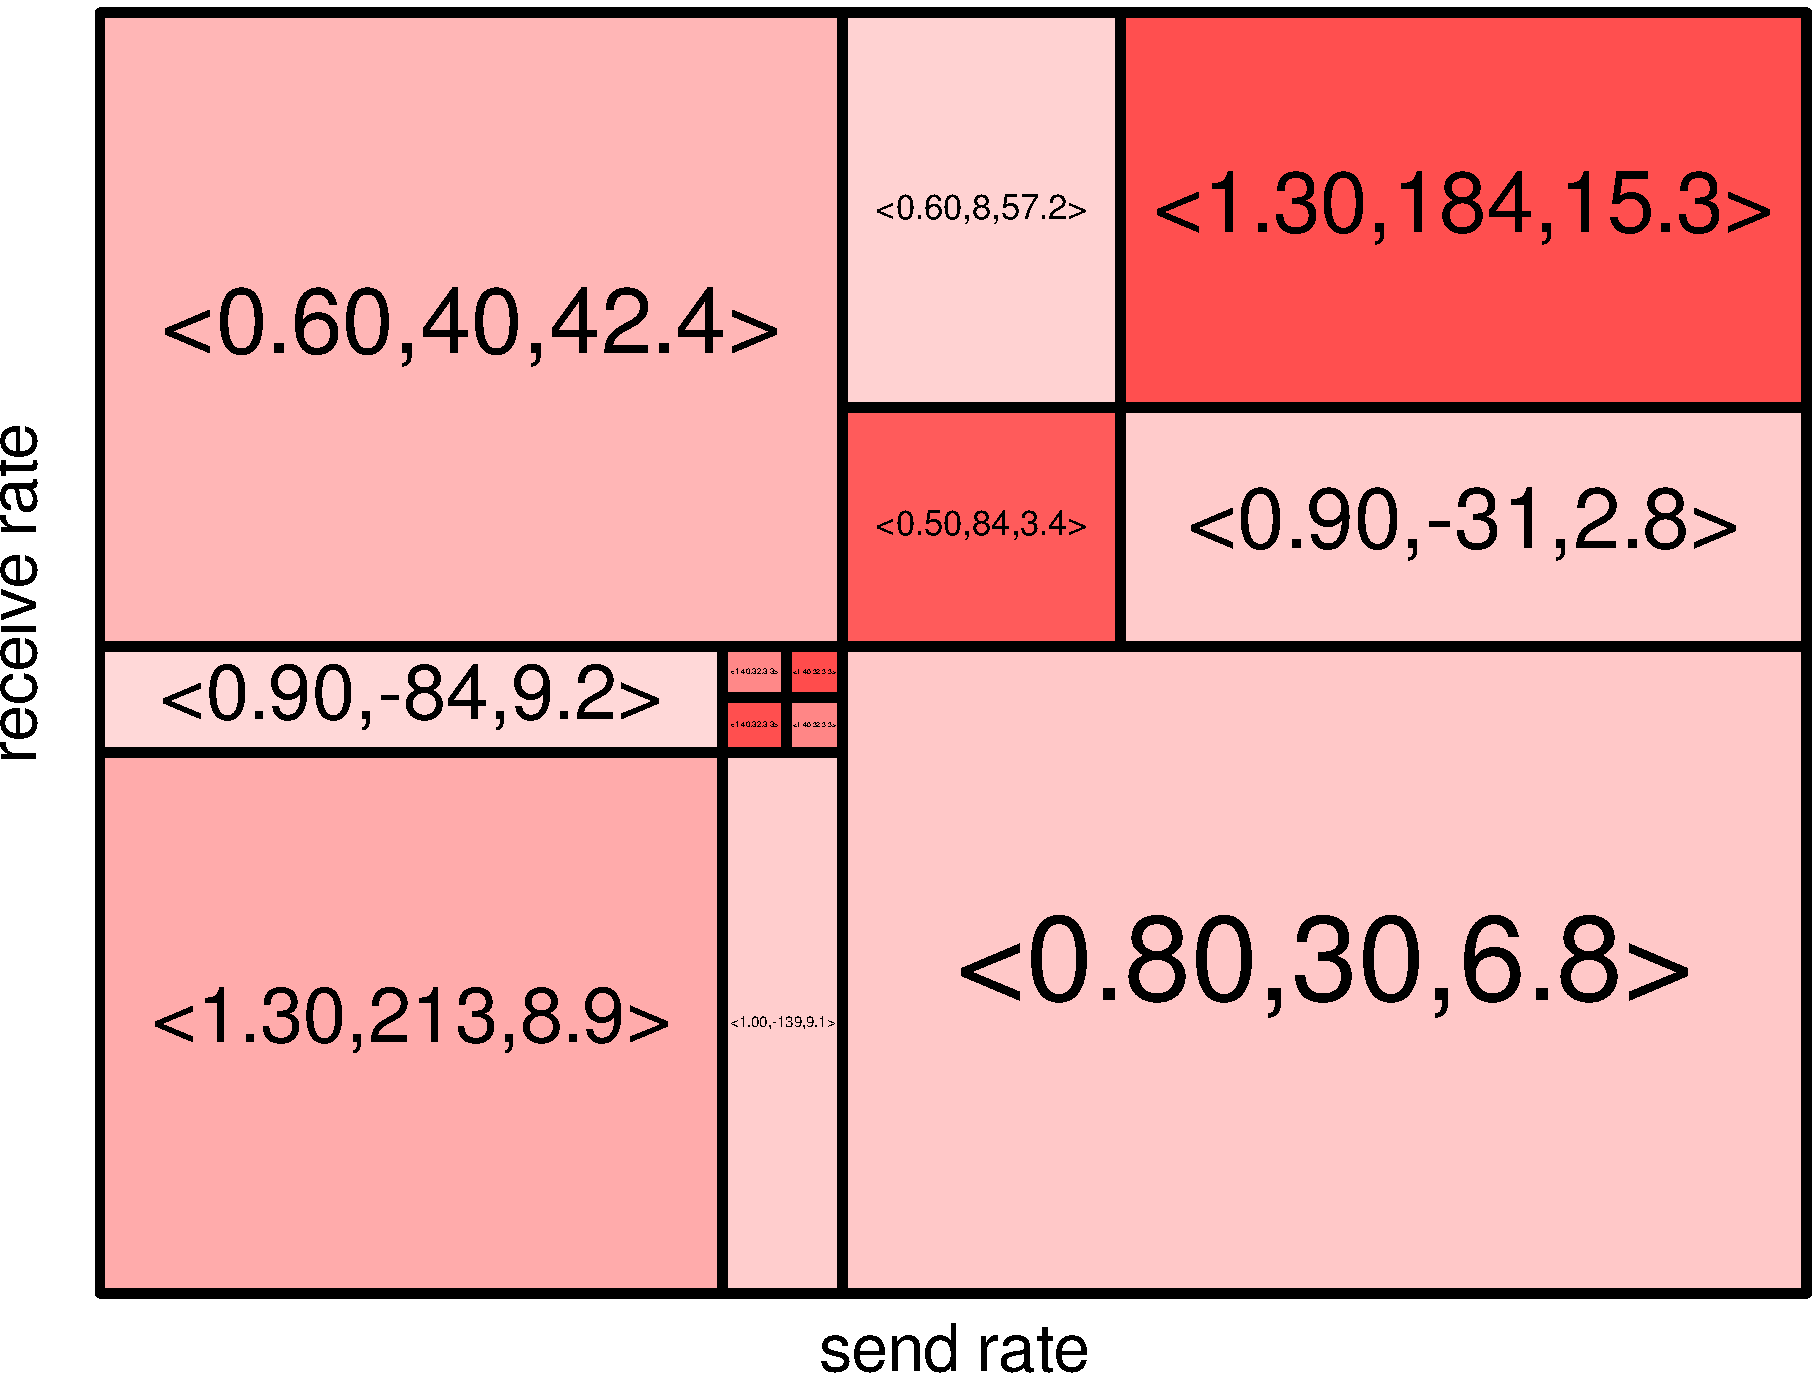
\includegraphics[width=8.5 cm]{remy-graph/graph/test12.pdf}

\end{centering}\end{frame}


\begin{frame}
\frametitle{Iterate}\begin{centering}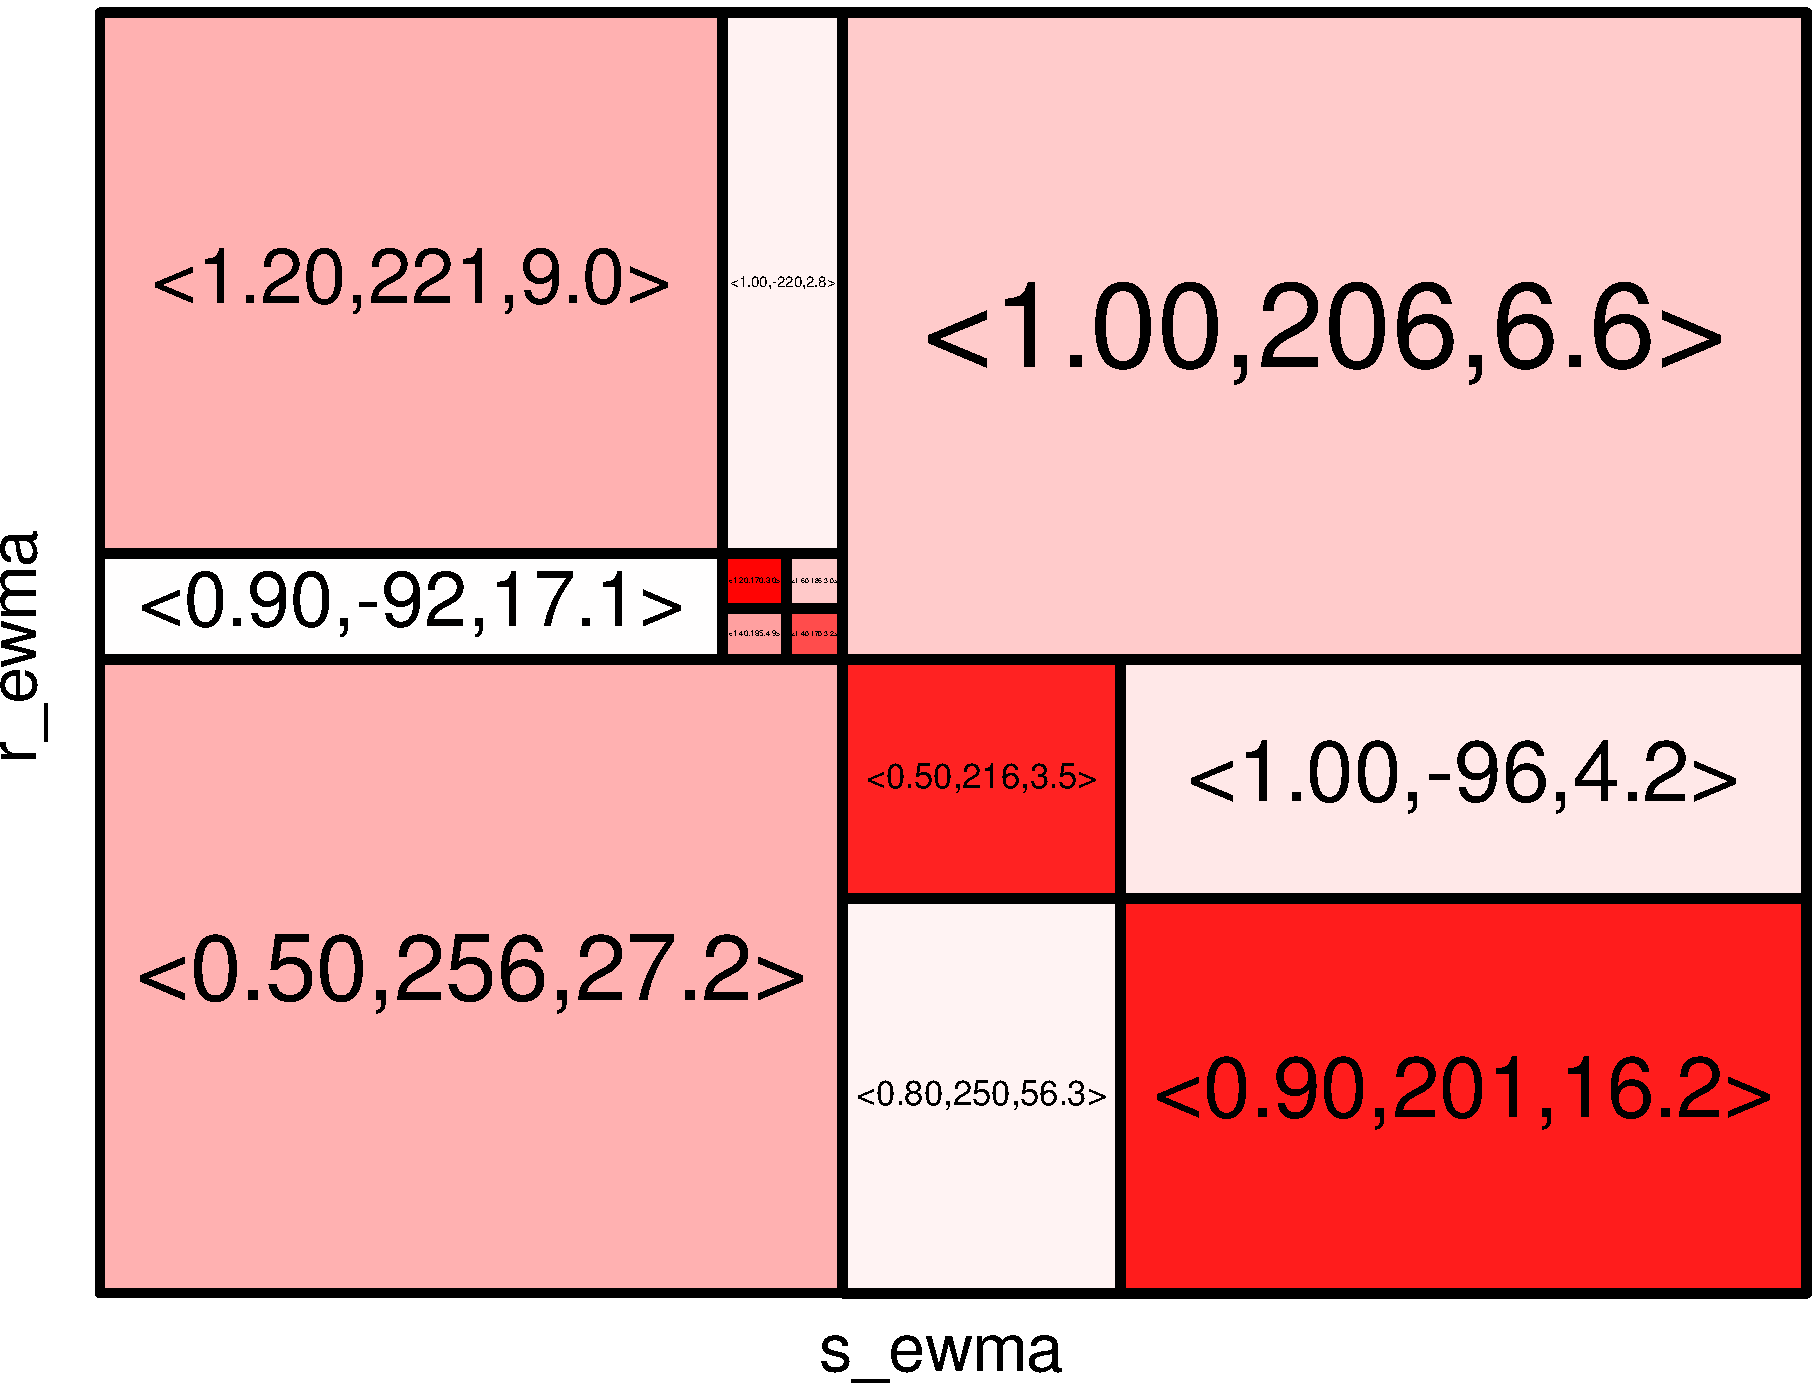
\includegraphics[width=8.5 cm]{remy-graph/graph/test13.pdf}

\end{centering}\end{frame}


\begin{frame}
\frametitle{Iterate}\begin{centering}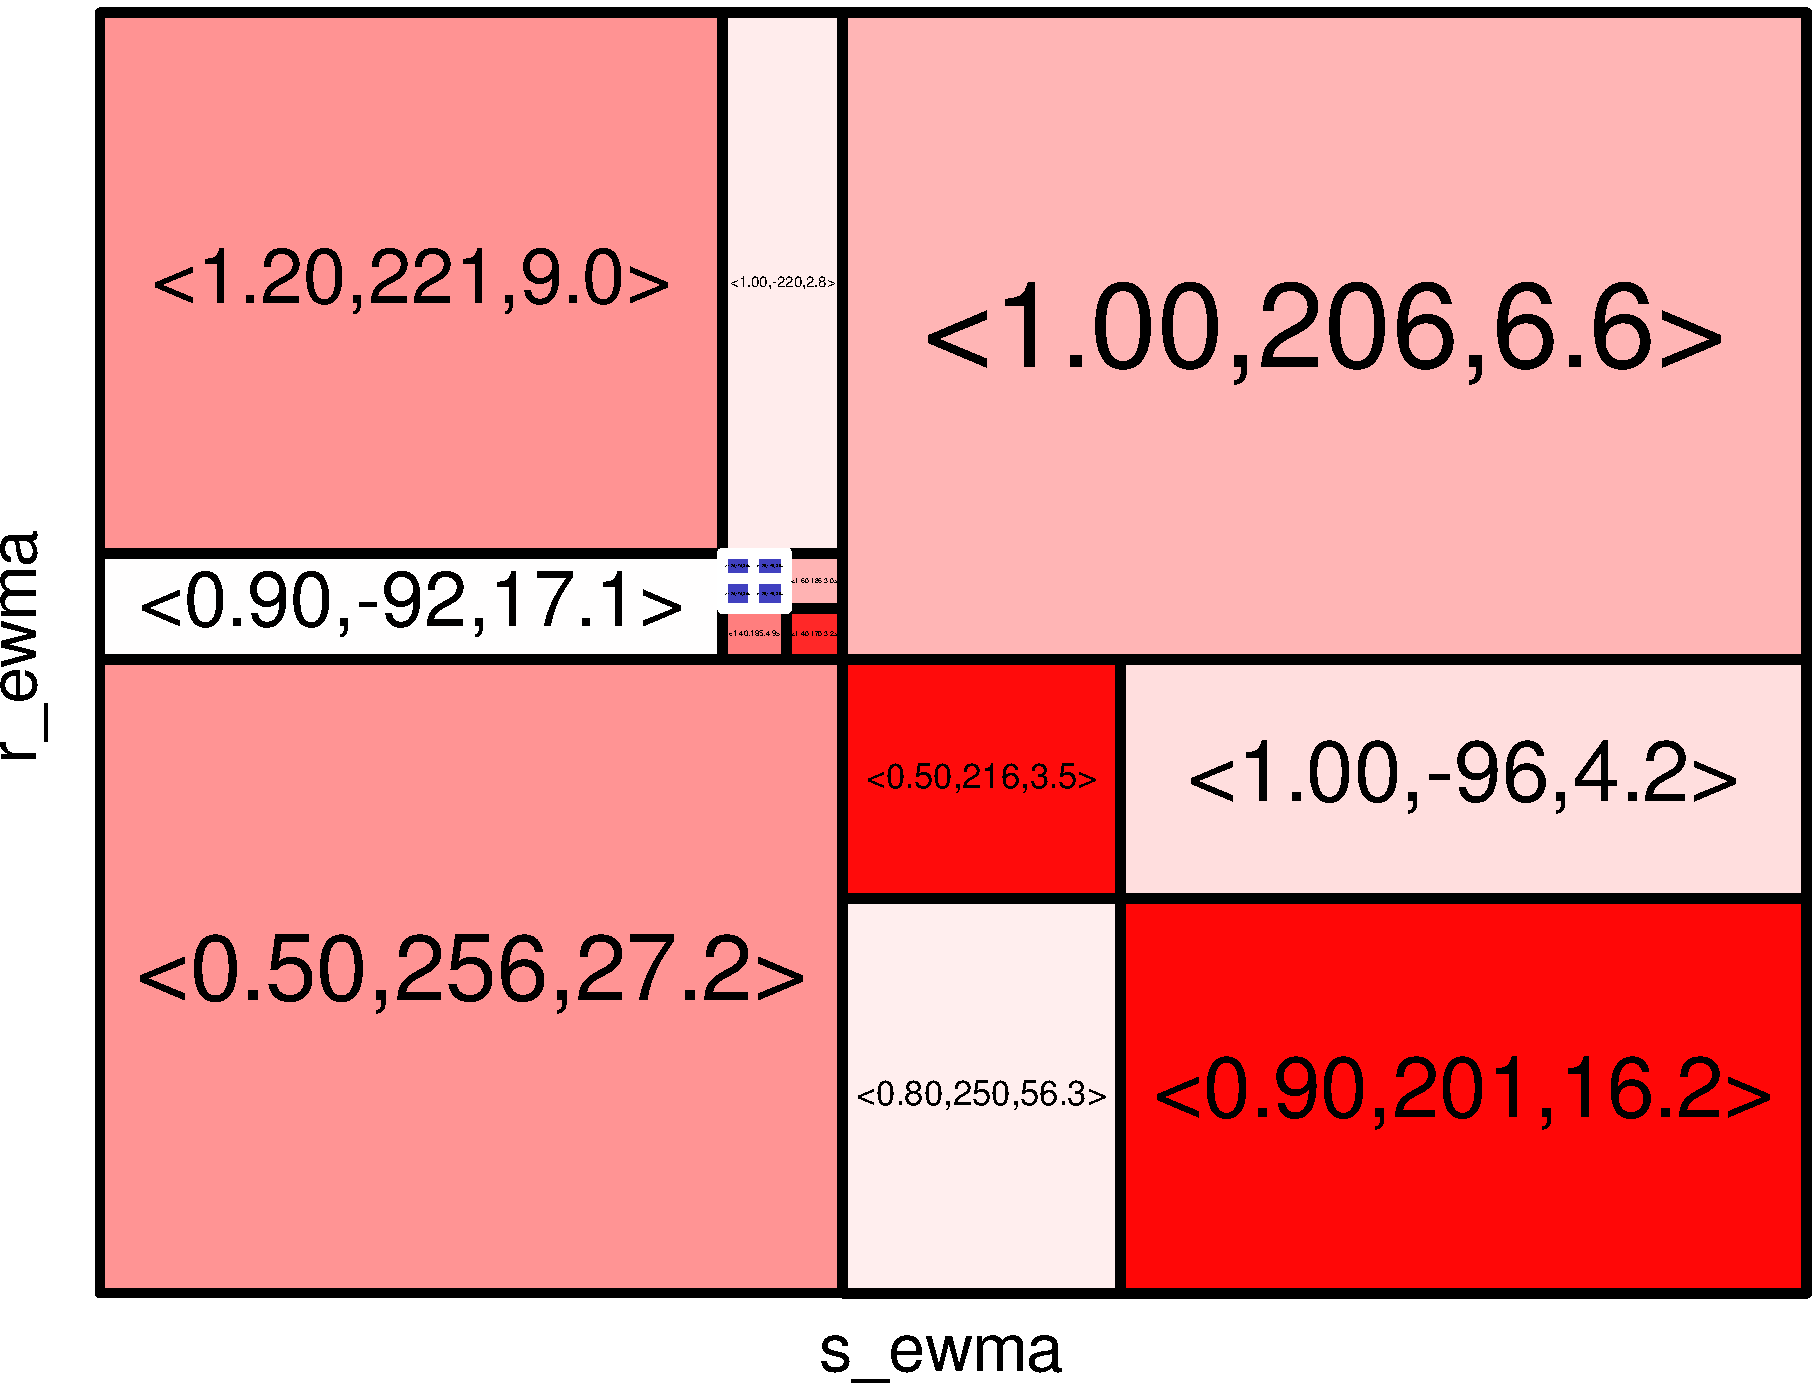
\includegraphics[width=8.5 cm]{remy-graph/graph/test14.pdf}

\end{centering}\end{frame}


\begin{frame}
\frametitle{Iterate}\begin{centering}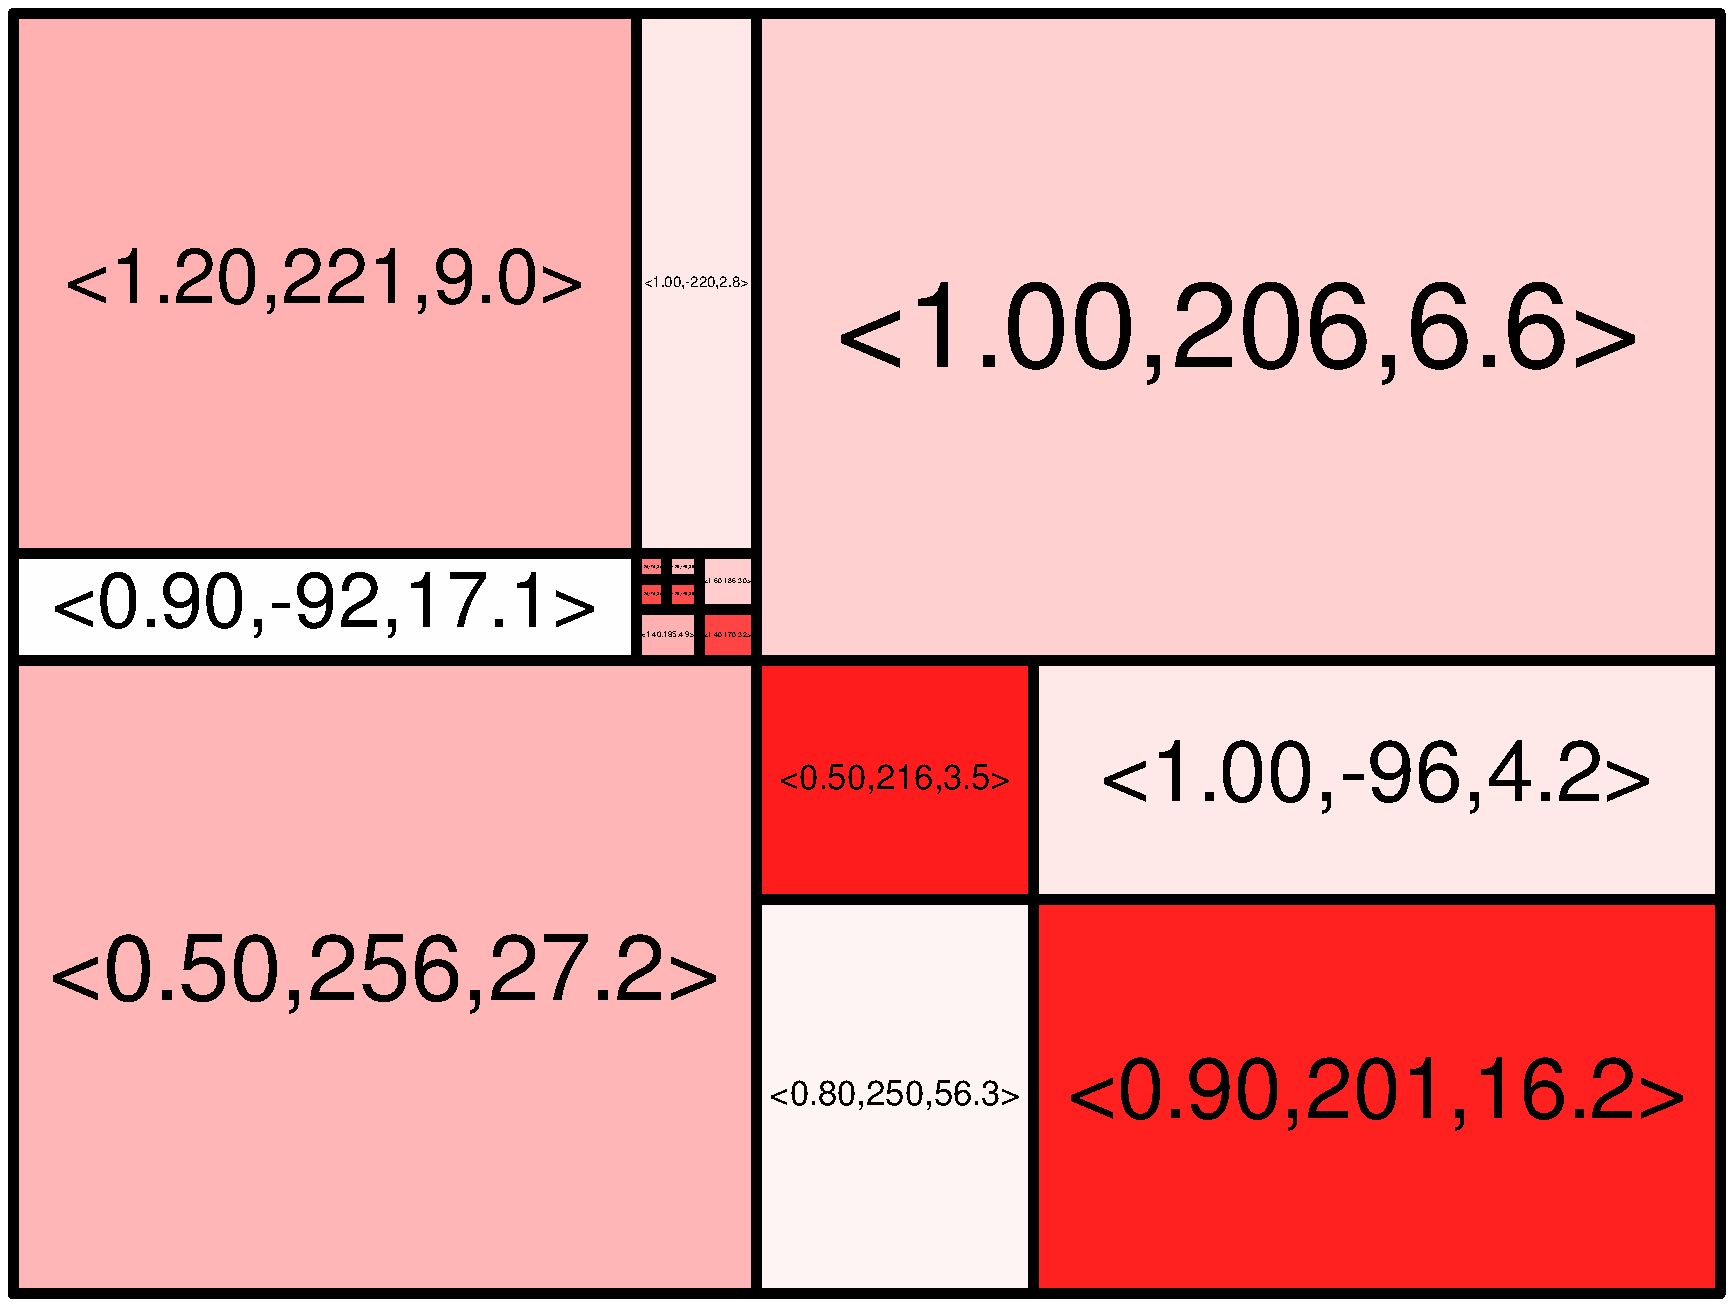
\includegraphics[width=8.5 cm]{remy-graph/graph/test15.pdf}

\end{centering}\end{frame}


\begin{frame}
\frametitle{Iterate}\begin{centering}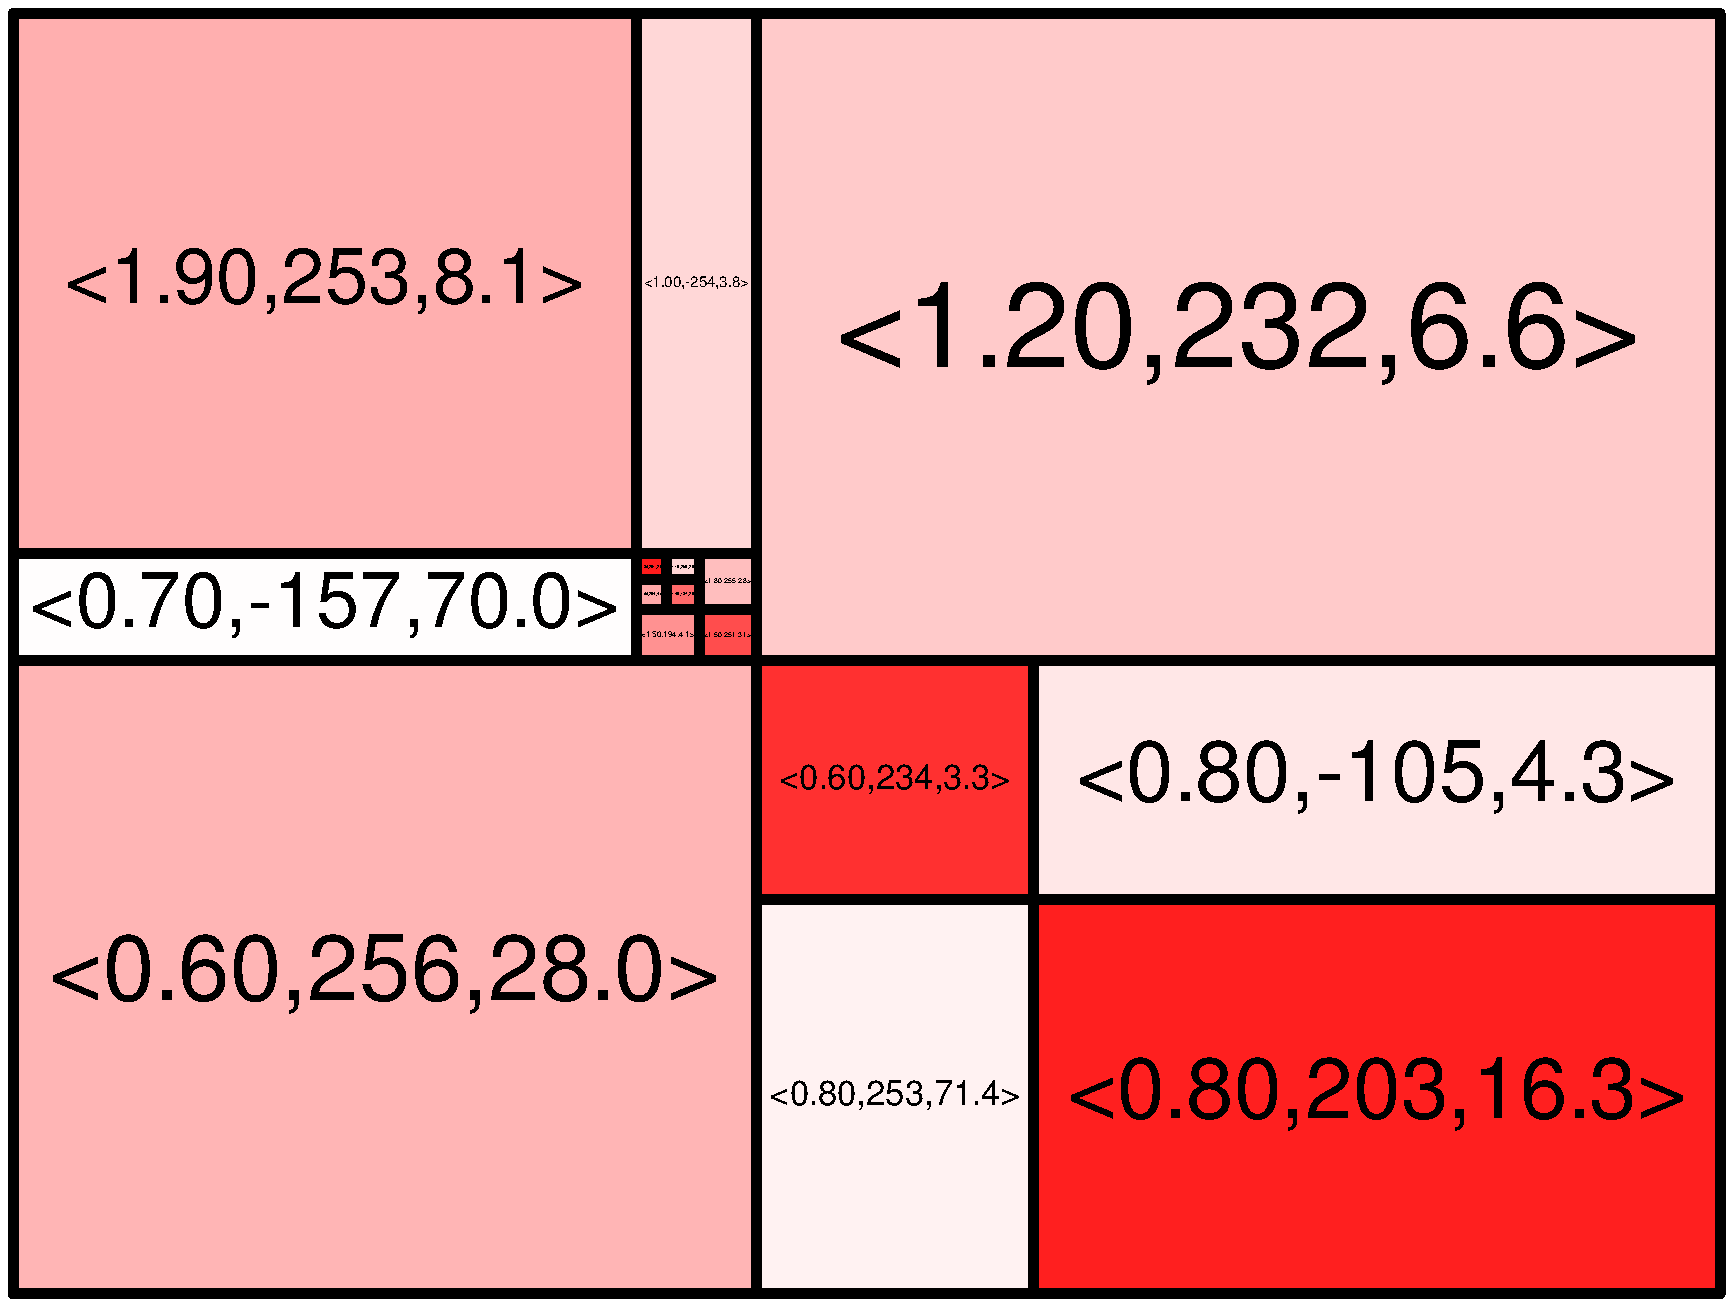
\includegraphics[width=8.5 cm]{remy-graph/graph/test16.pdf}

\end{centering}\end{frame}


\begin{frame}
\frametitle{Iterate}\begin{centering}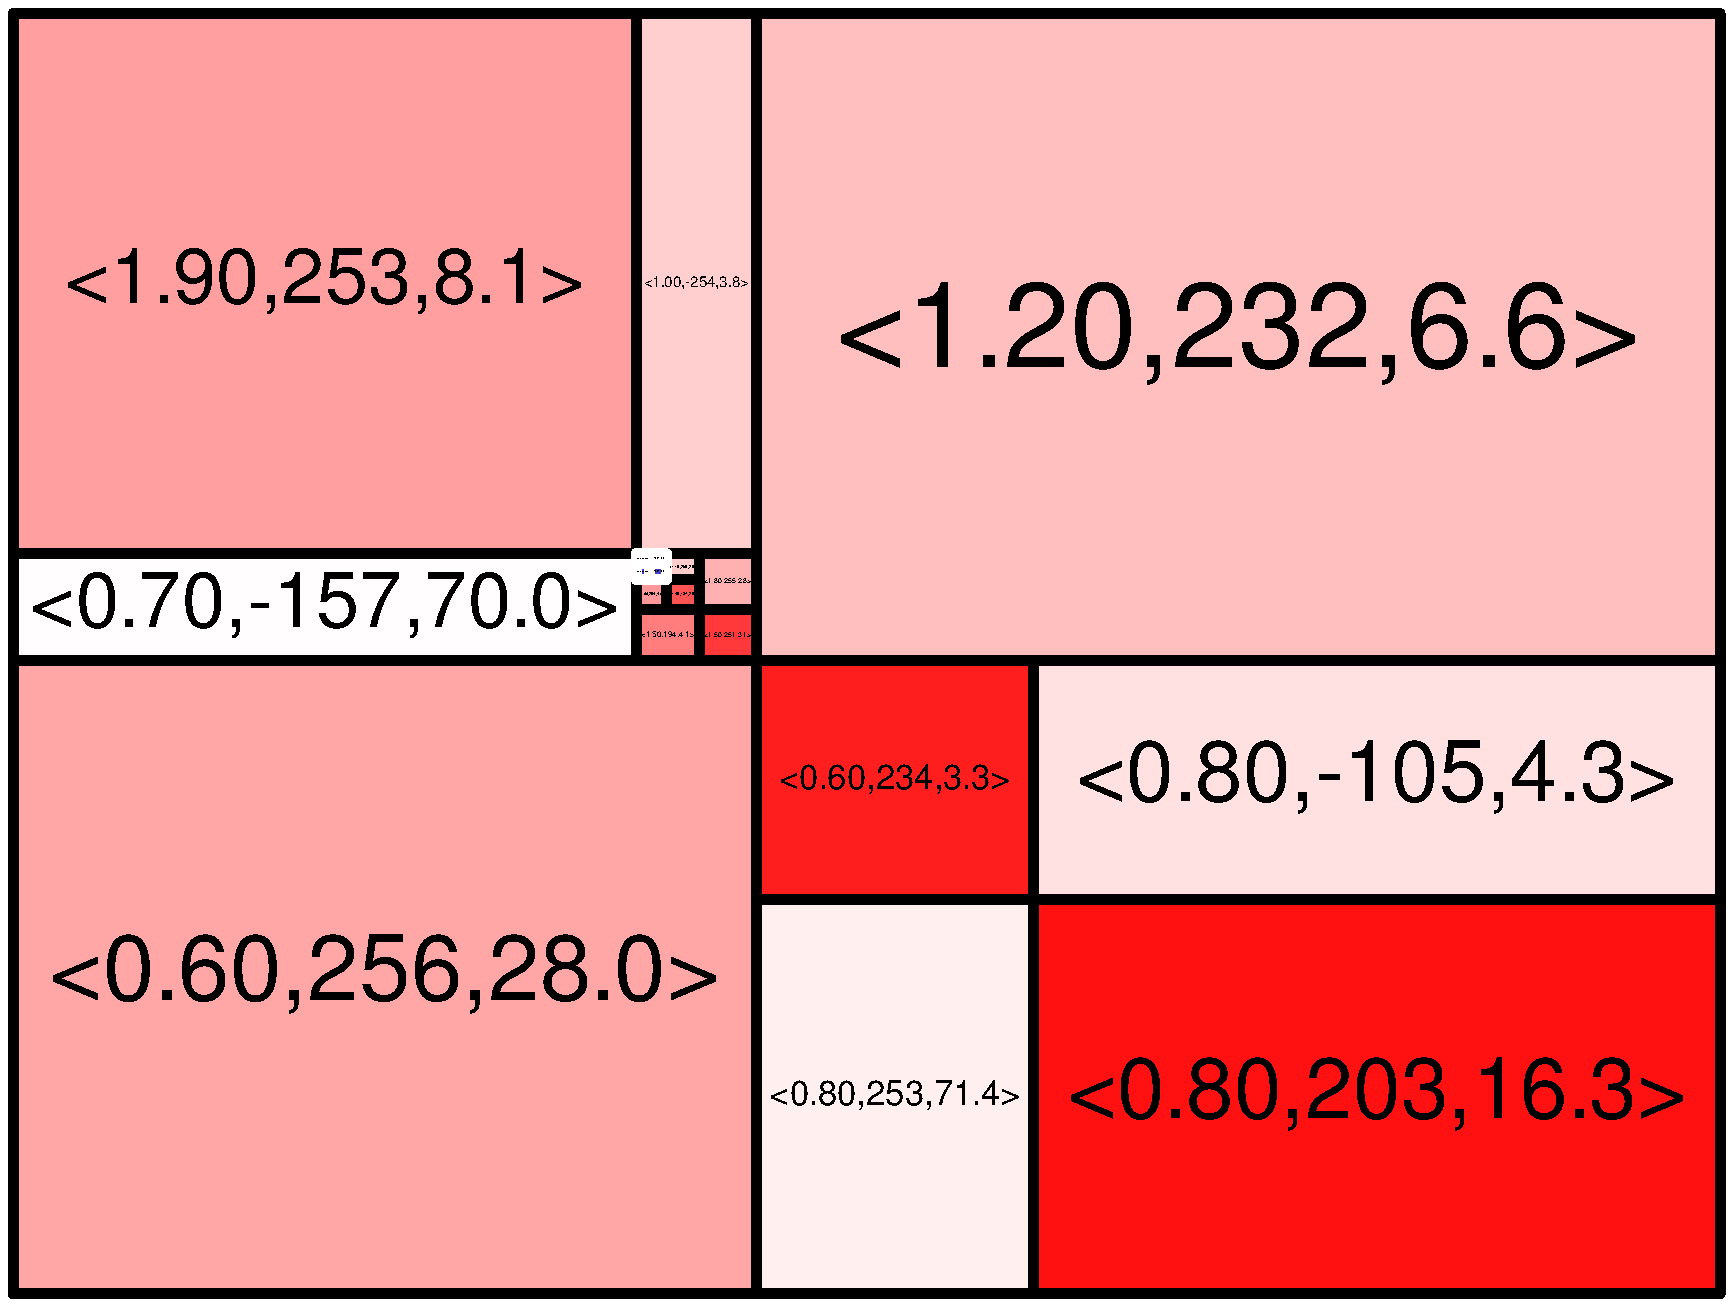
\includegraphics[width=8.5 cm]{remy-graph/graph/test17.pdf}

\end{centering}\end{frame}


\begin{frame}
\frametitle{Iterate}\begin{centering}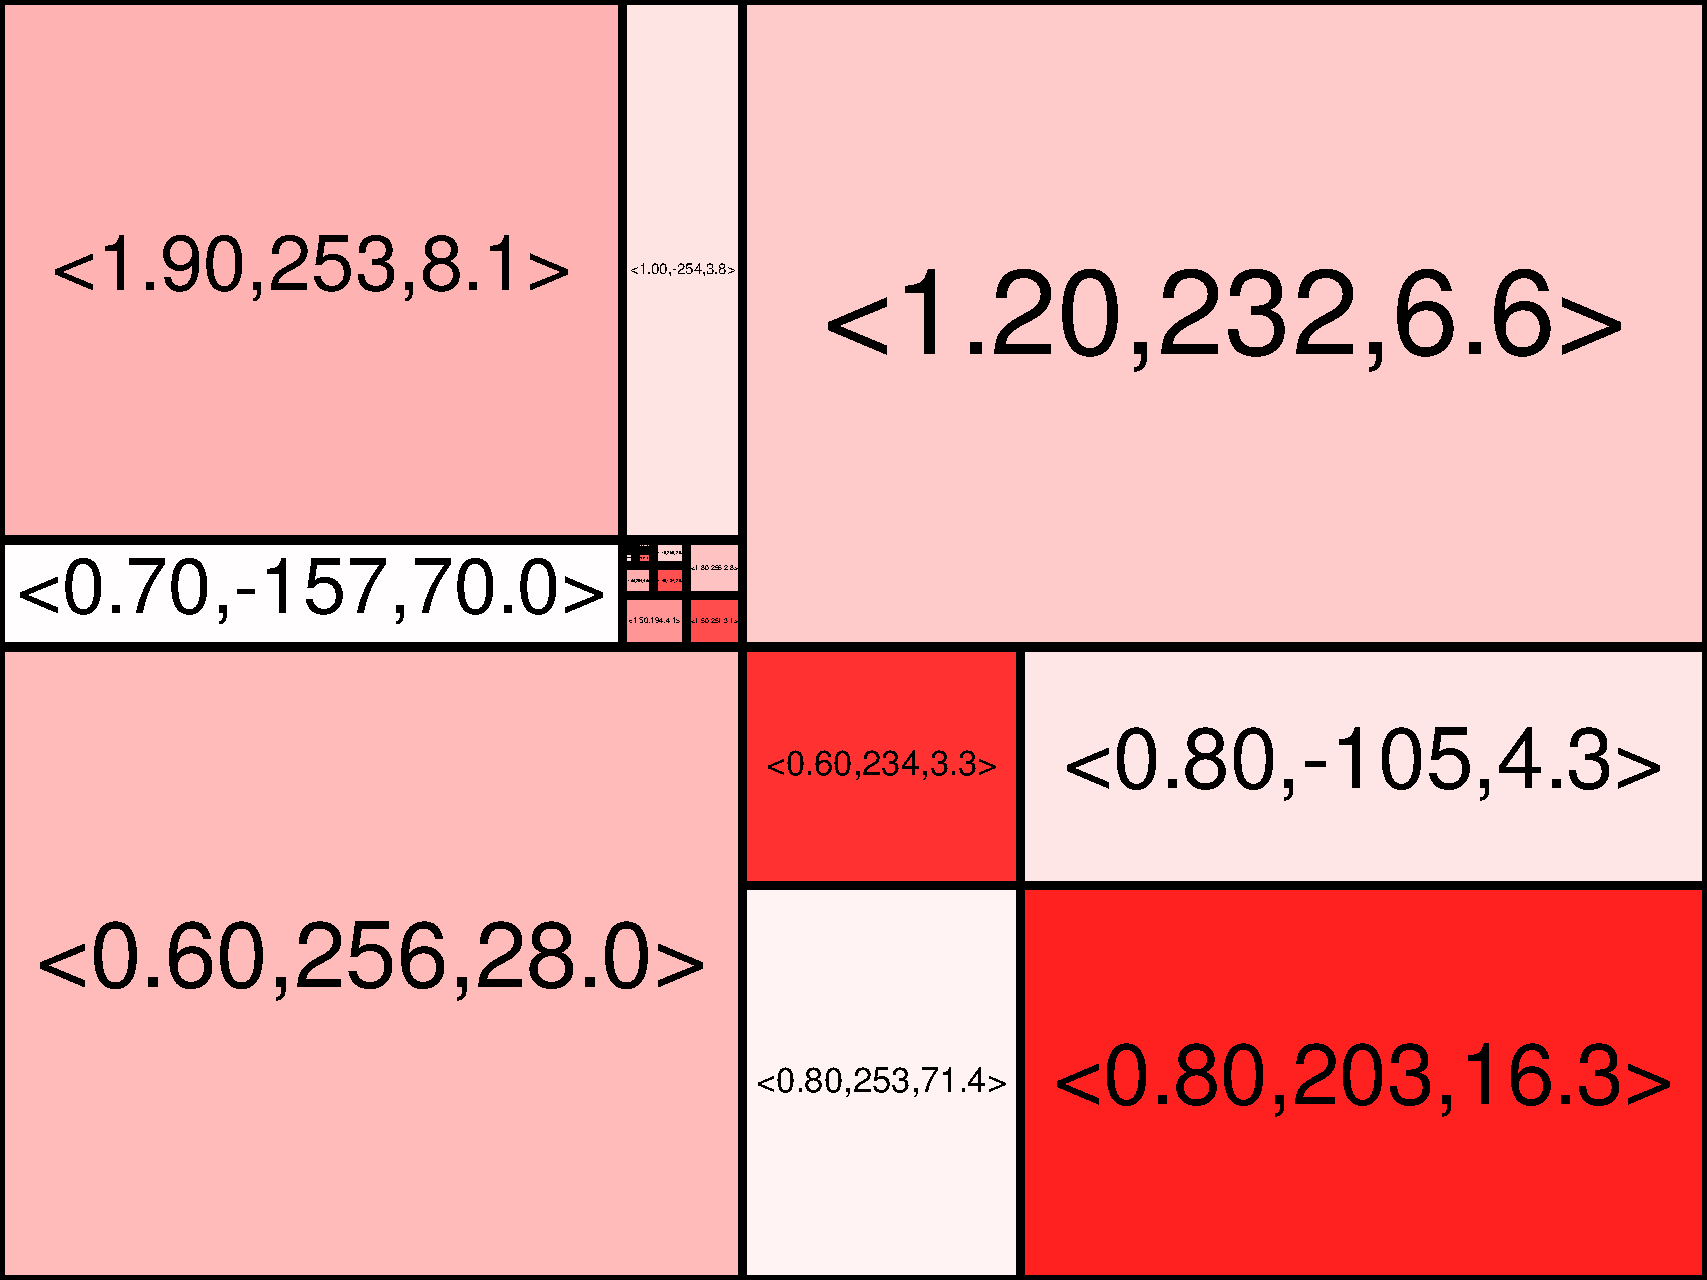
\includegraphics[width=8.5 cm]{remy-graph/graph/test18.pdf}

\end{centering}\end{frame}


\begin{frame}
\frametitle{Iterate}\begin{centering}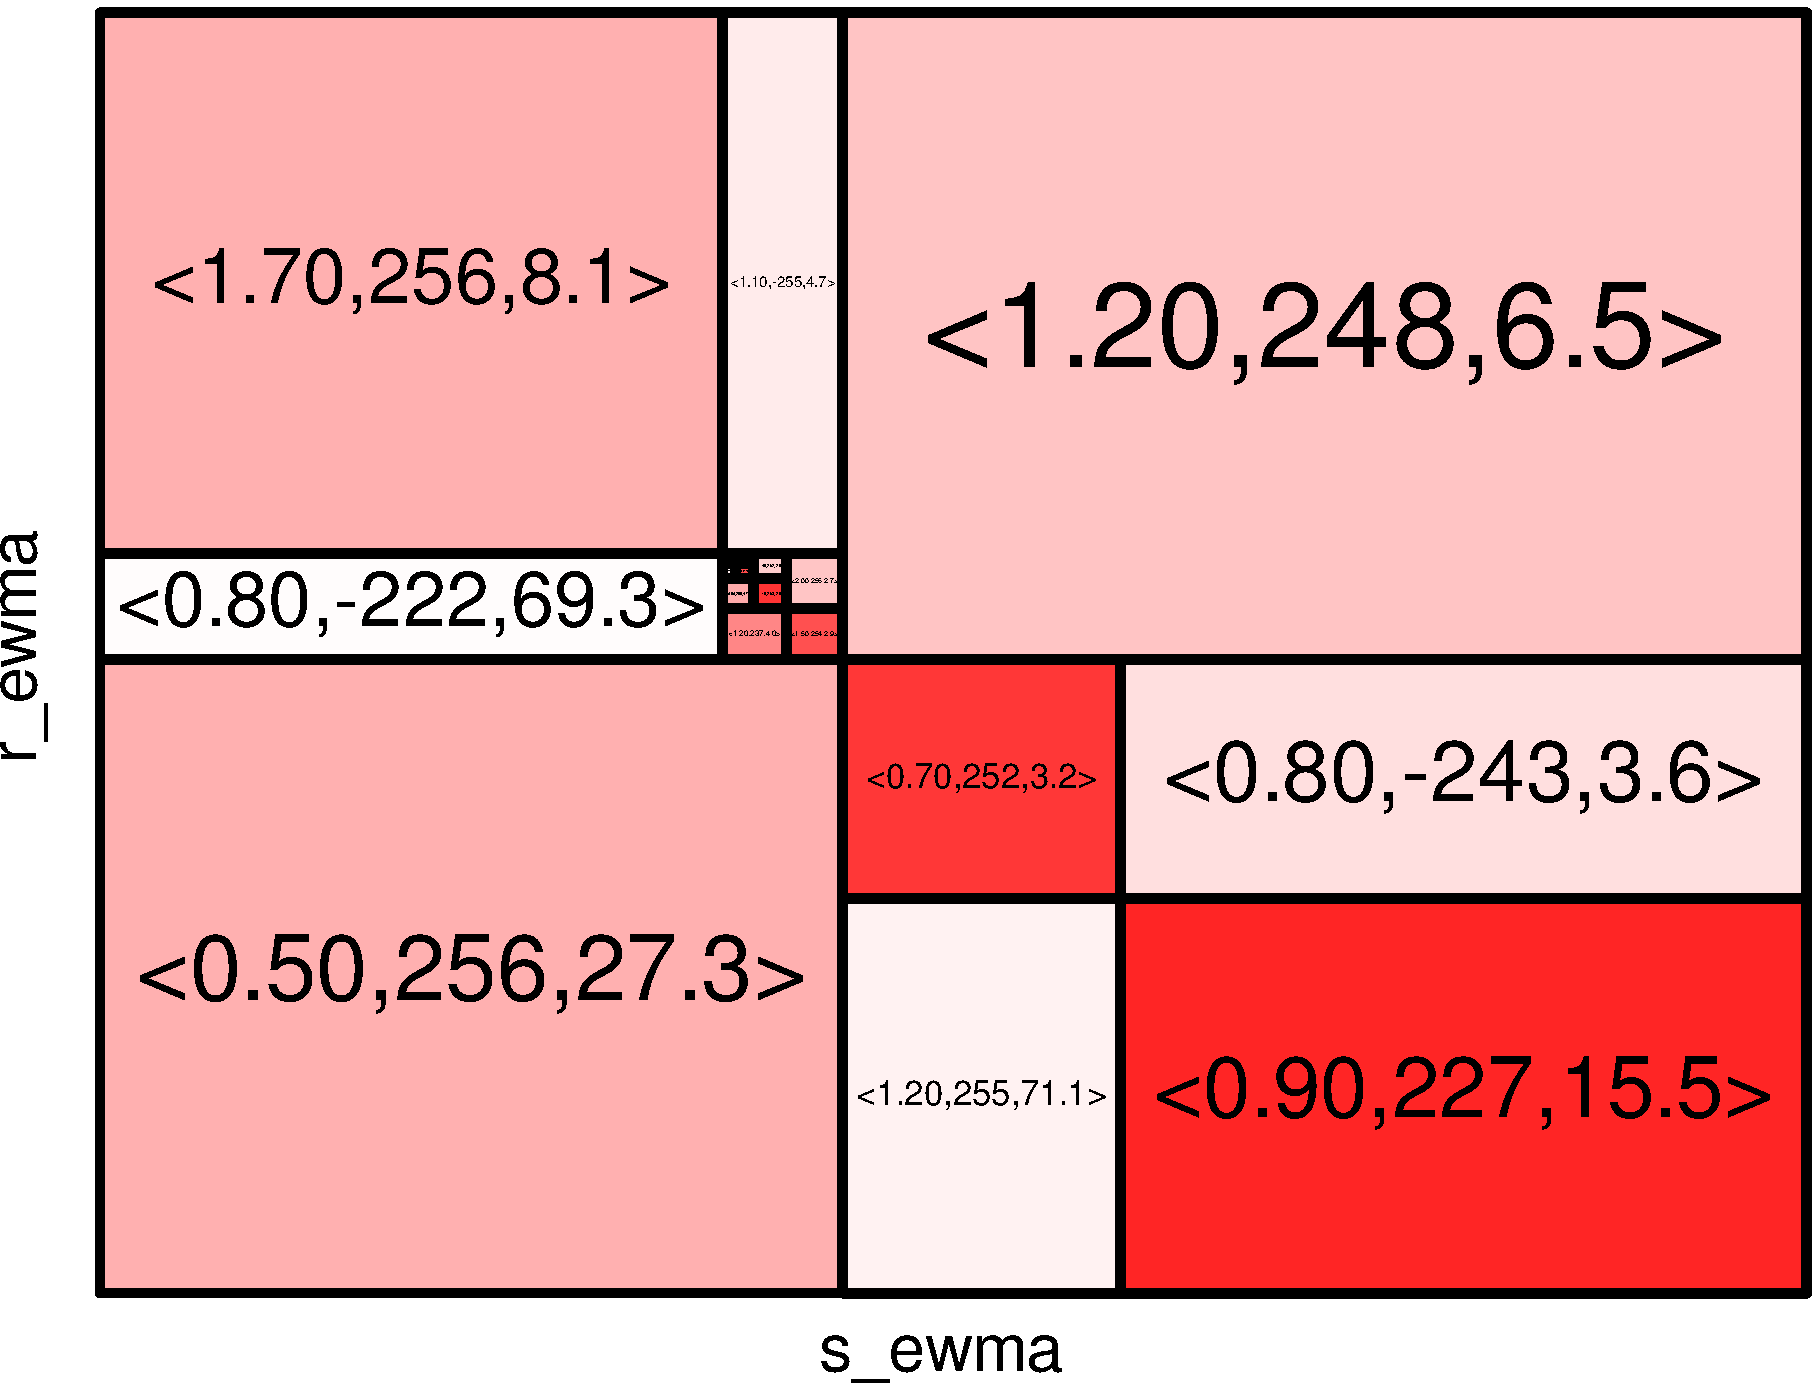
\includegraphics[width=8.5 cm]{remy-graph/graph/test19.pdf}

\end{centering}\end{frame}


\begin{frame}
\frametitle{Iterate}\begin{centering}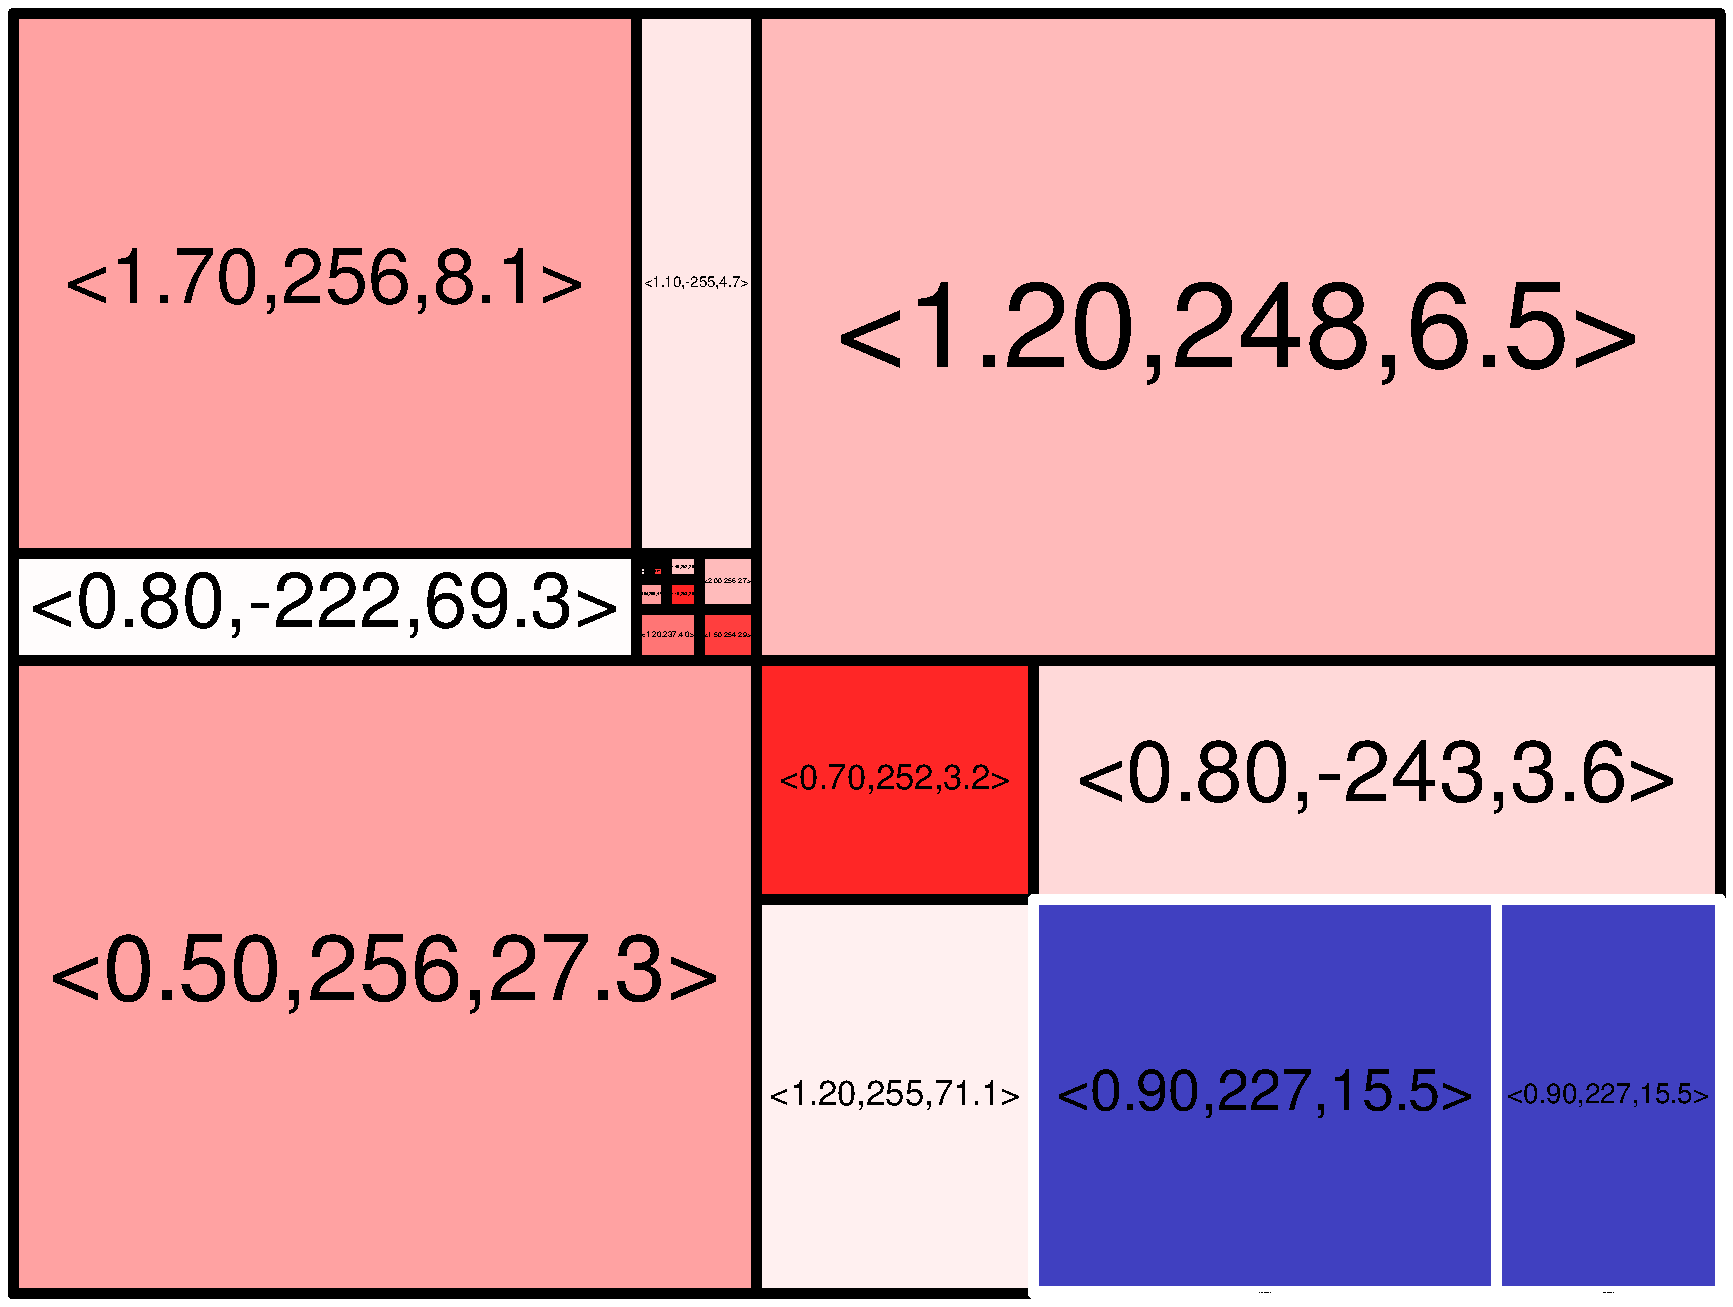
\includegraphics[width=8.5 cm]{remy-graph/graph/test20.pdf}

\end{centering}\end{frame}


\begin{frame}
\frametitle{Iterate}\begin{centering}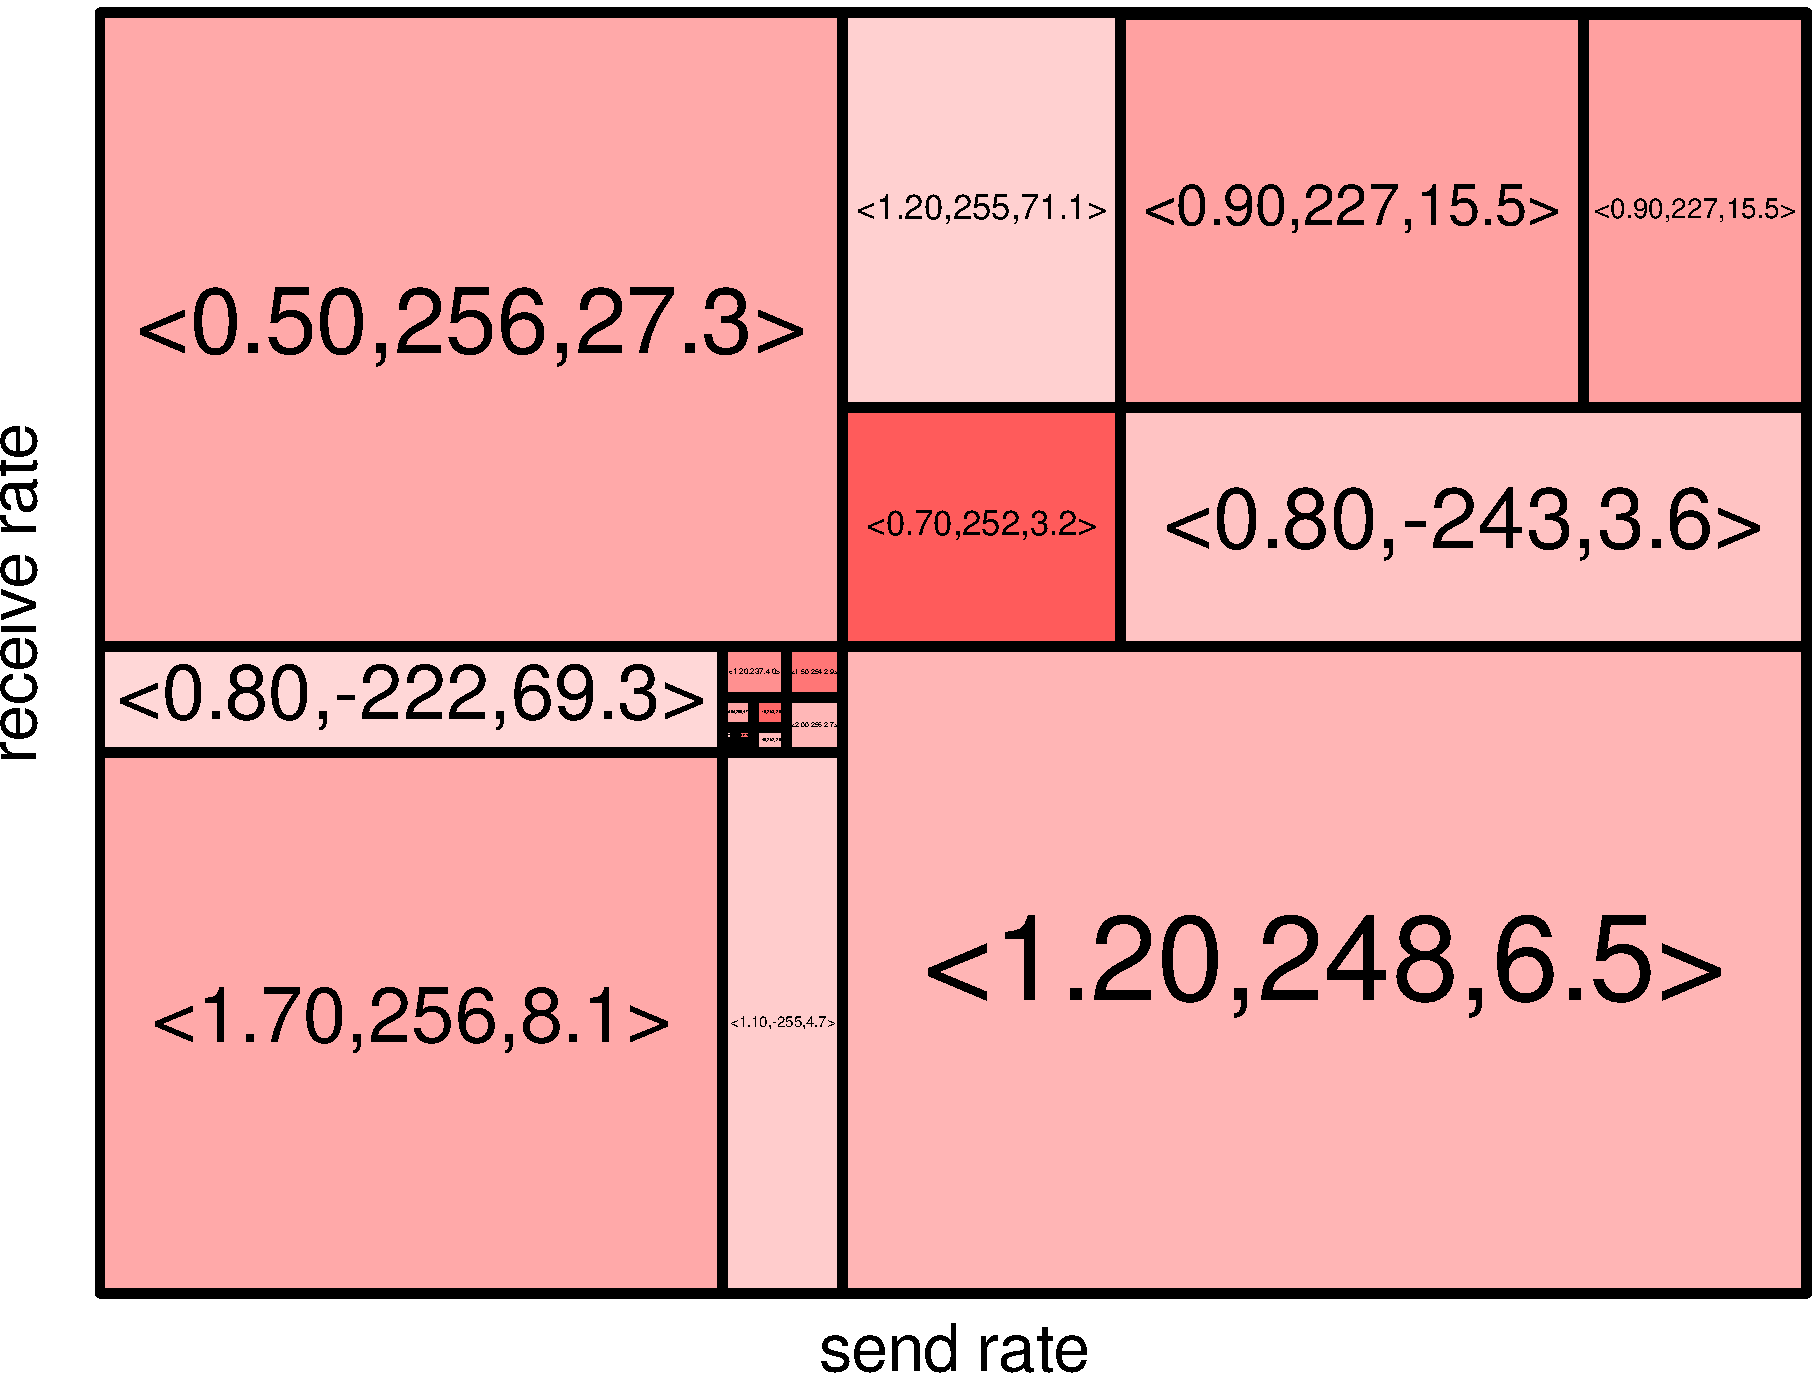
\includegraphics[width=8.5 cm]{remy-graph/graph/test21.pdf}

\end{centering}\end{frame}


\begin{frame}
\frametitle{Iterate}\begin{centering}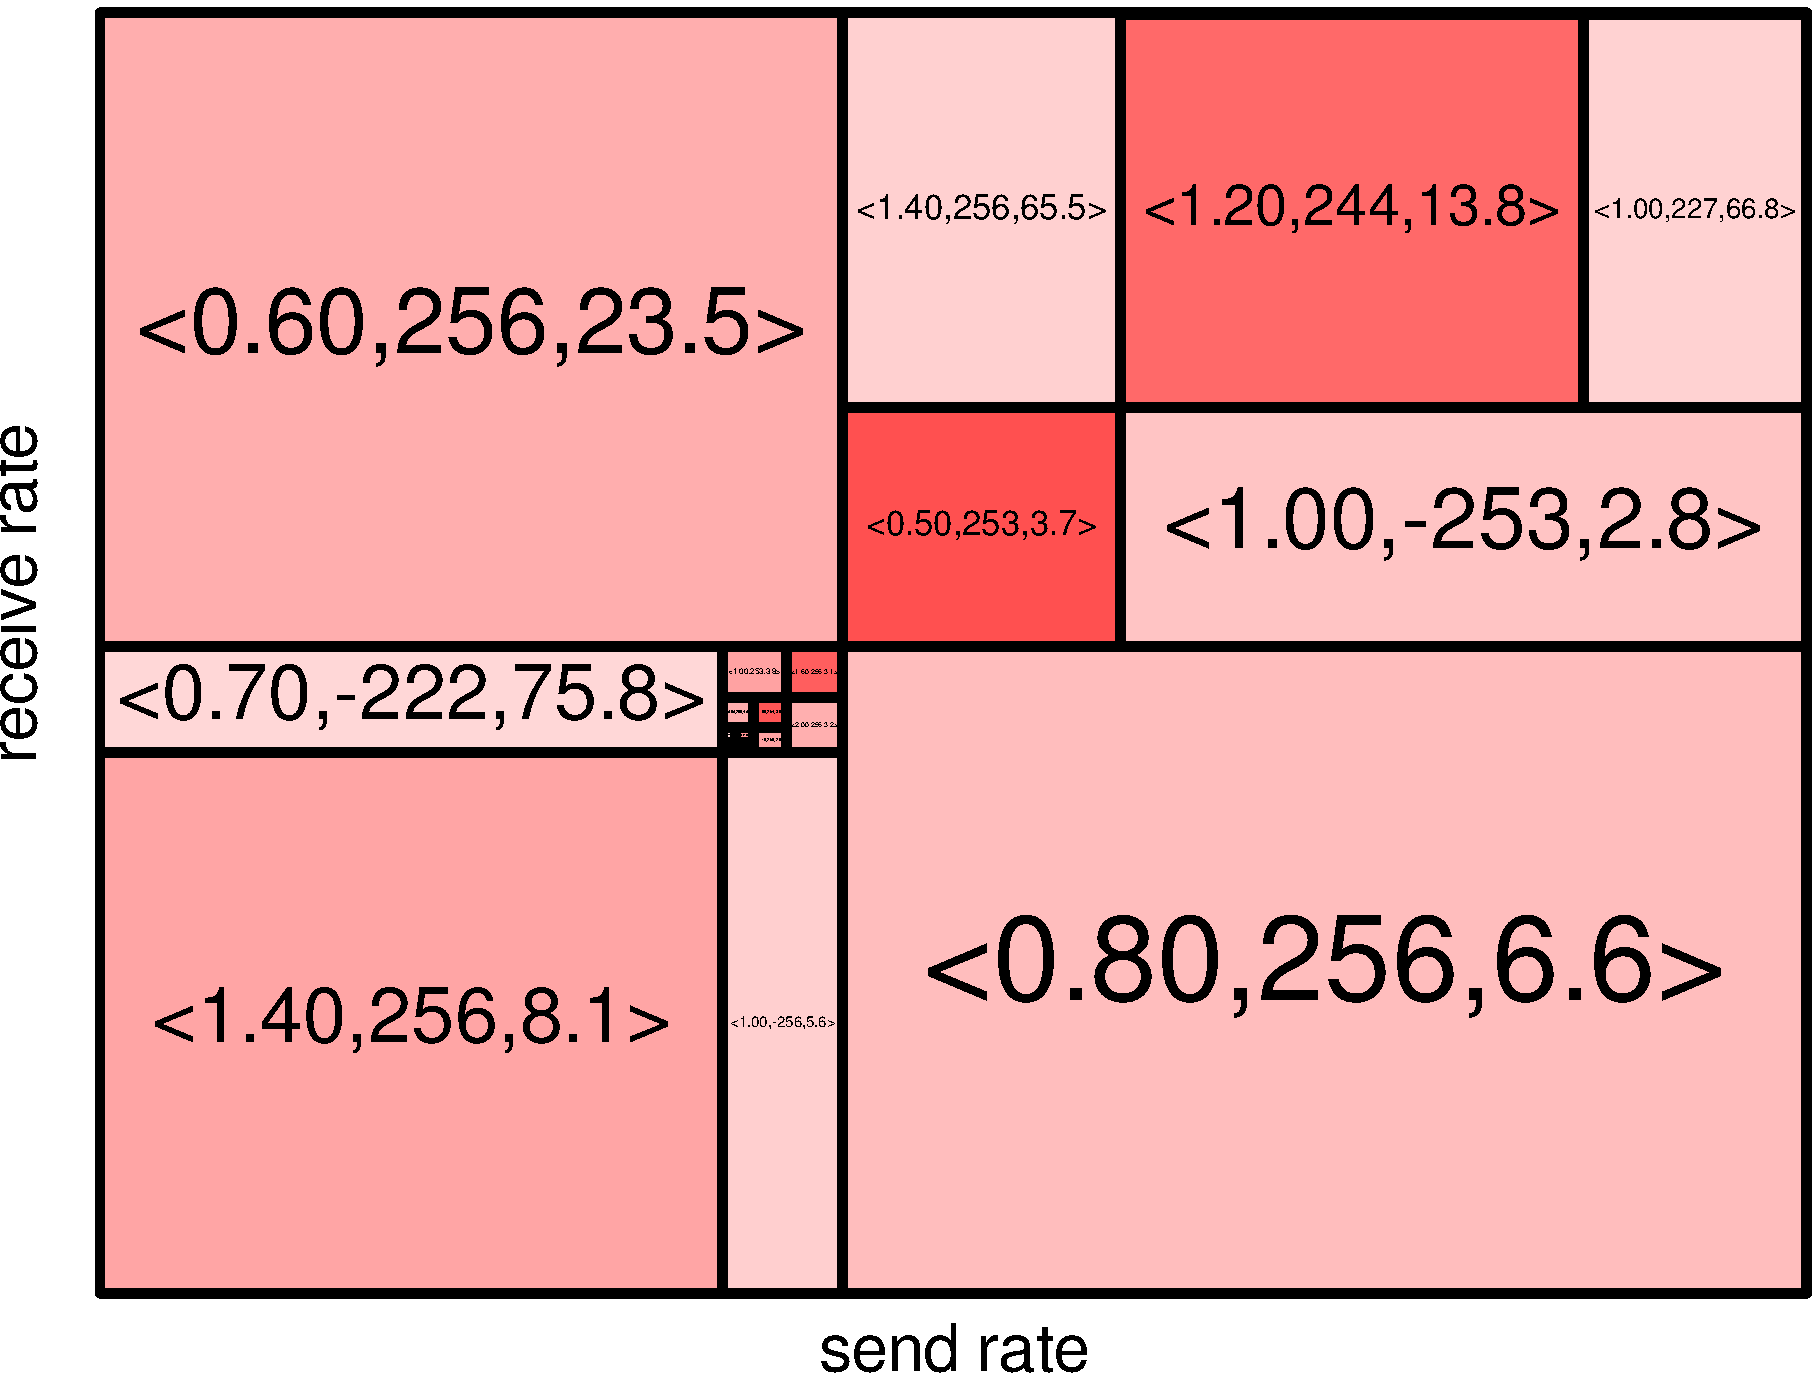
\includegraphics[width=8.5 cm]{remy-graph/graph/test22.pdf}

\end{centering}\end{frame}


\begin{frame}
\frametitle{Iterate}\begin{centering}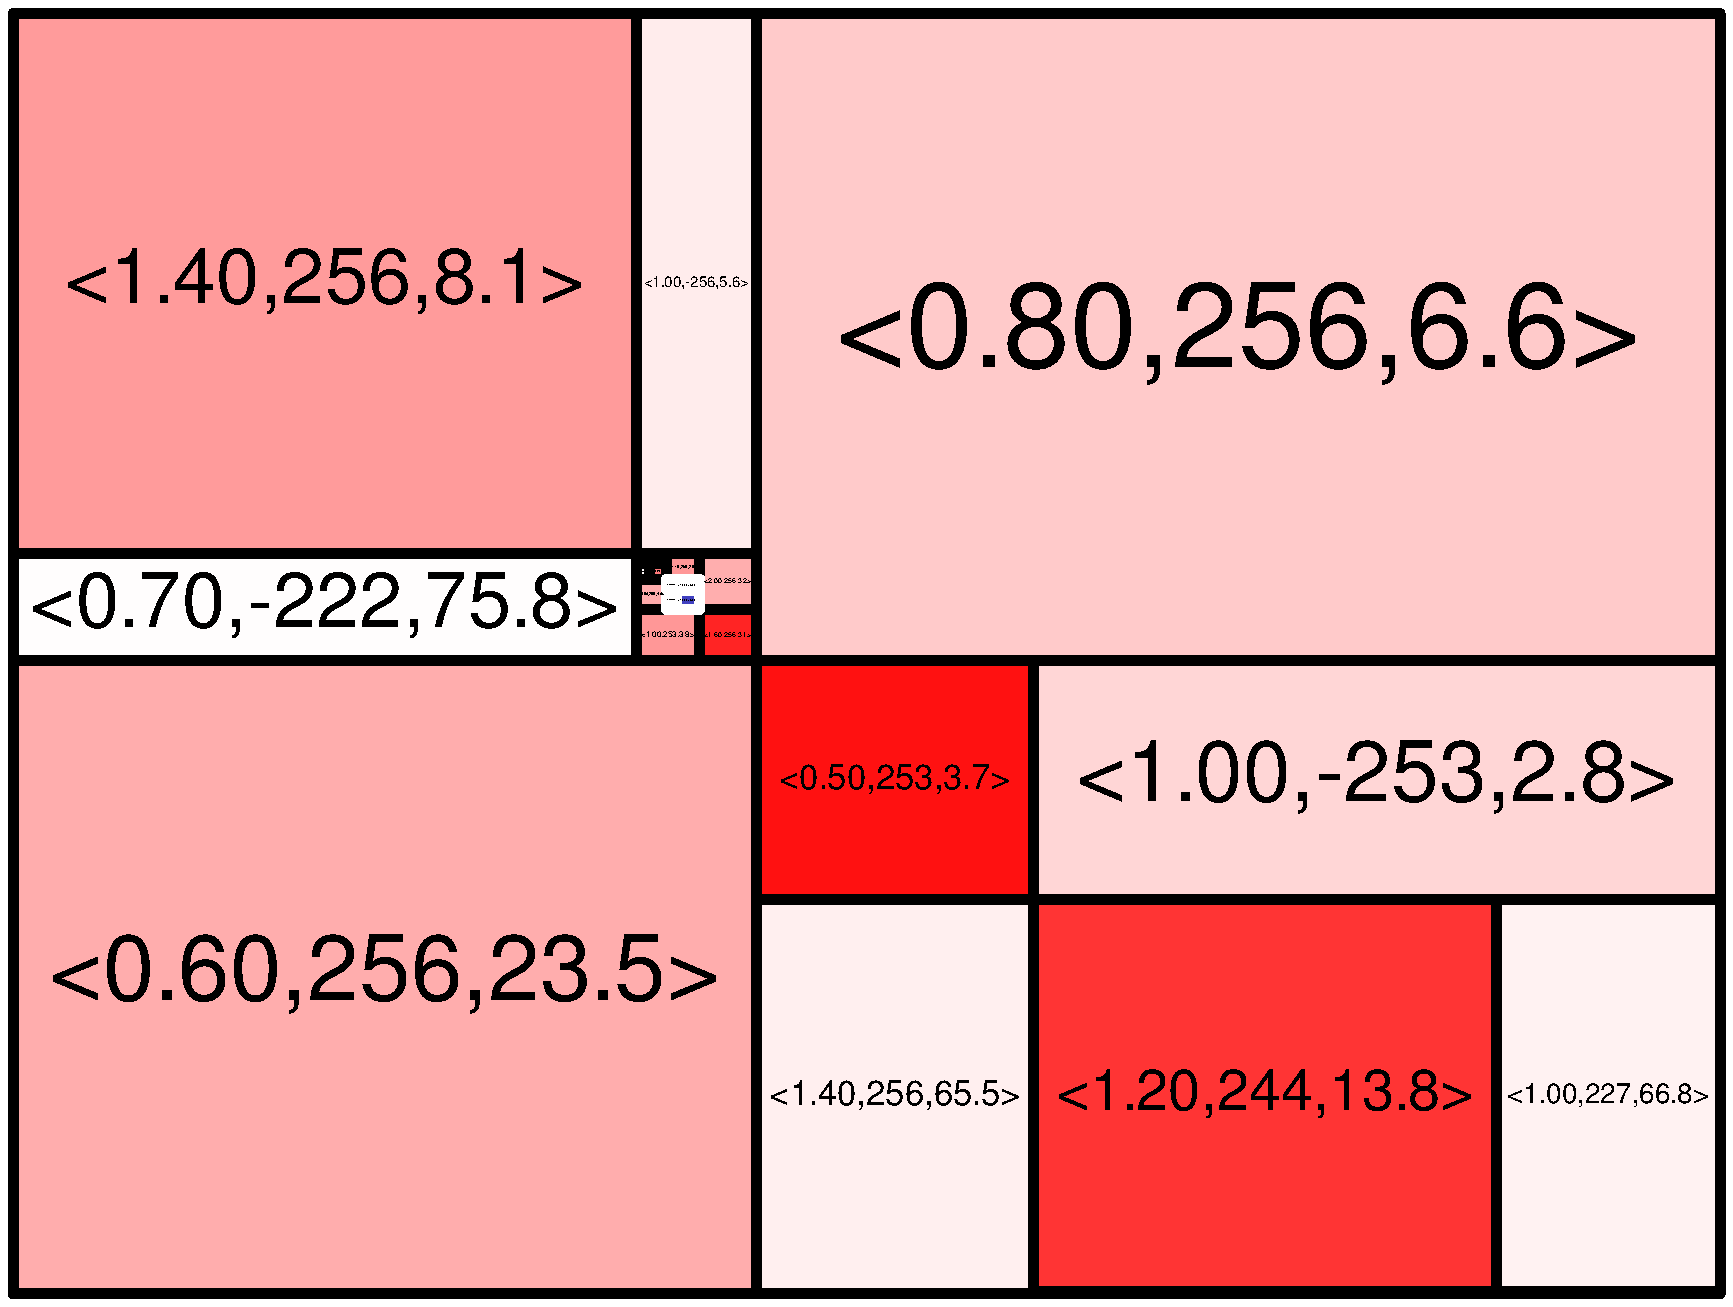
\includegraphics[width=8.5 cm]{remy-graph/graph/test23.pdf}

\end{centering}\end{frame}


\begin{frame}
\frametitle{Iterate}\begin{centering}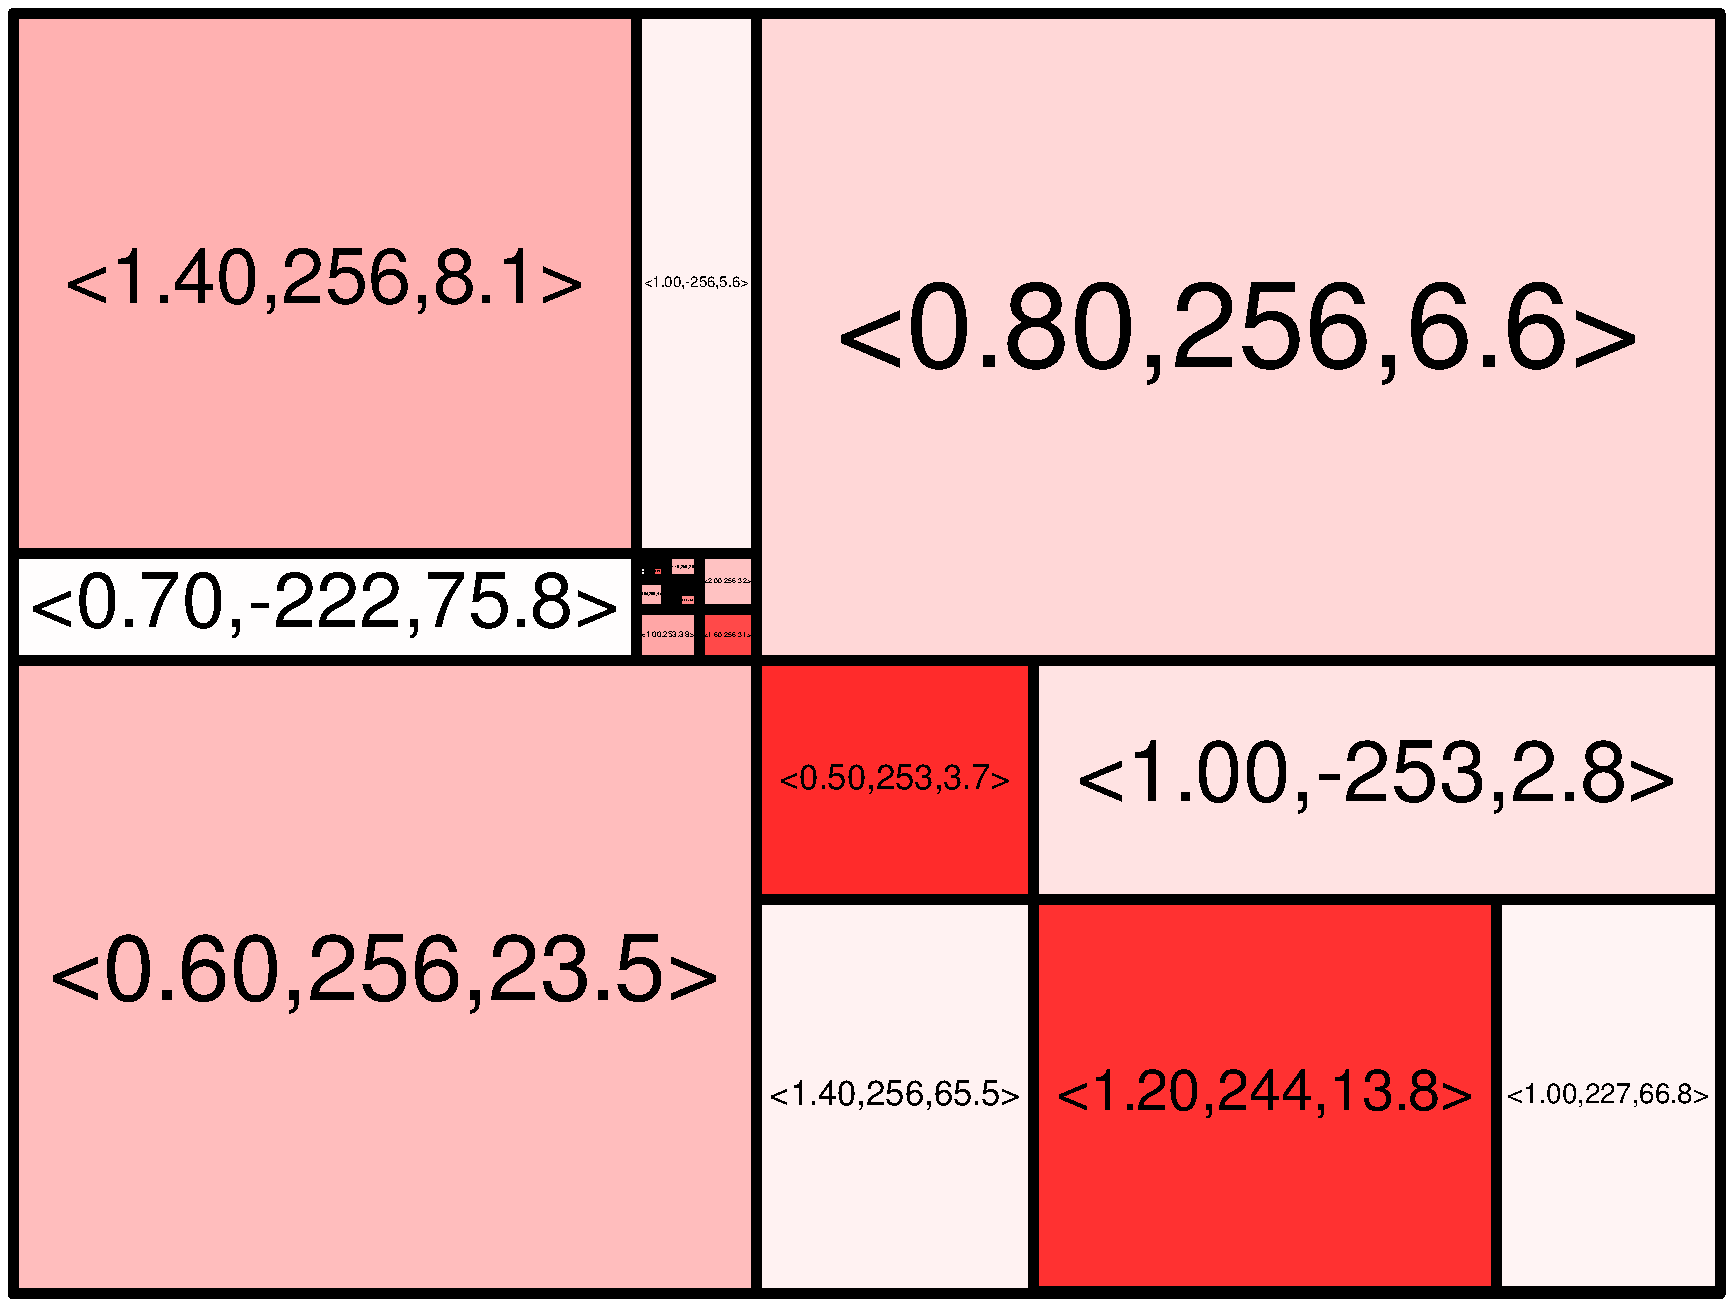
\includegraphics[width=8.5 cm]{remy-graph/graph/test24.pdf}

\end{centering}\end{frame}


\begin{frame}
\frametitle{Iterate}\begin{centering}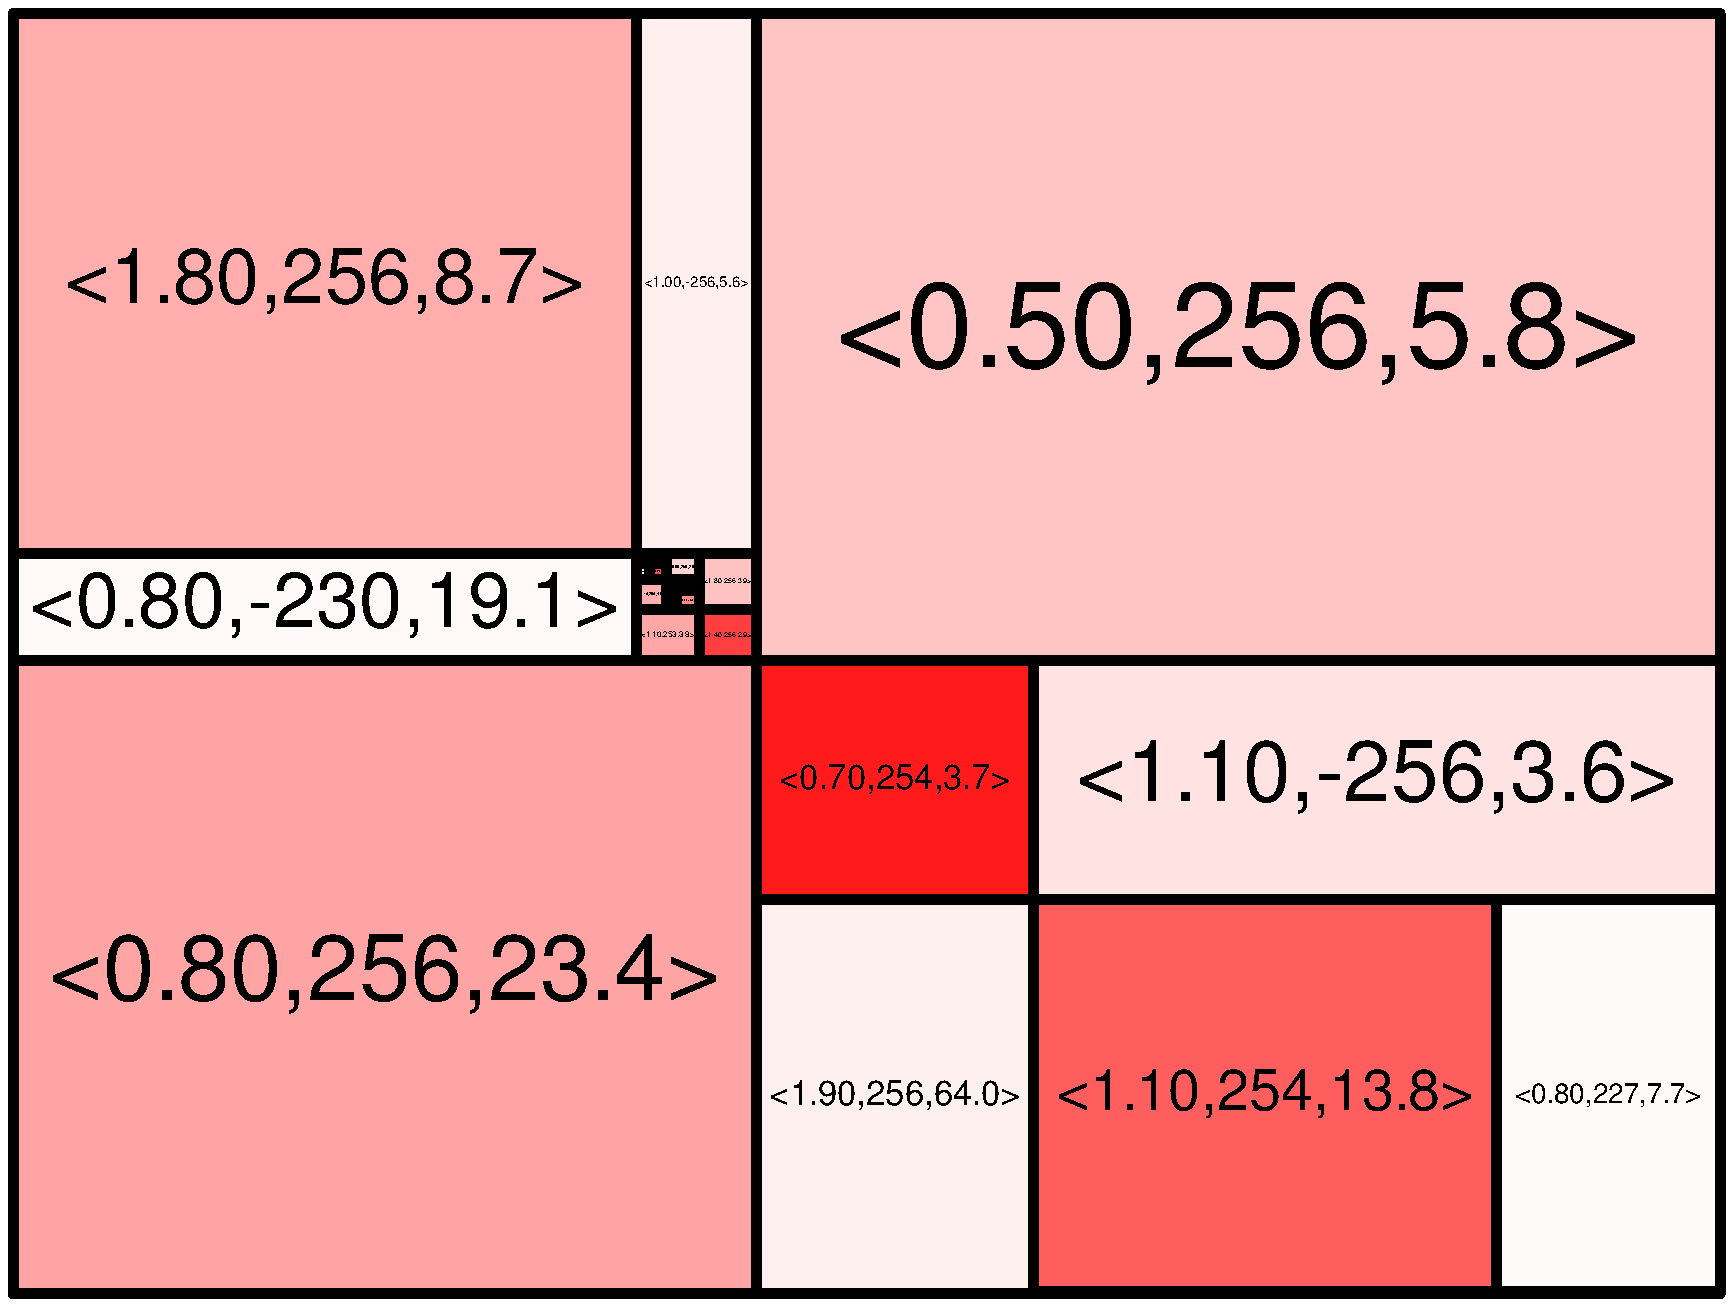
\includegraphics[width=8.5 cm]{remy-graph/graph/test25.pdf}

\end{centering}\end{frame}


\begin{frame}
\frametitle{Iterate}\begin{centering}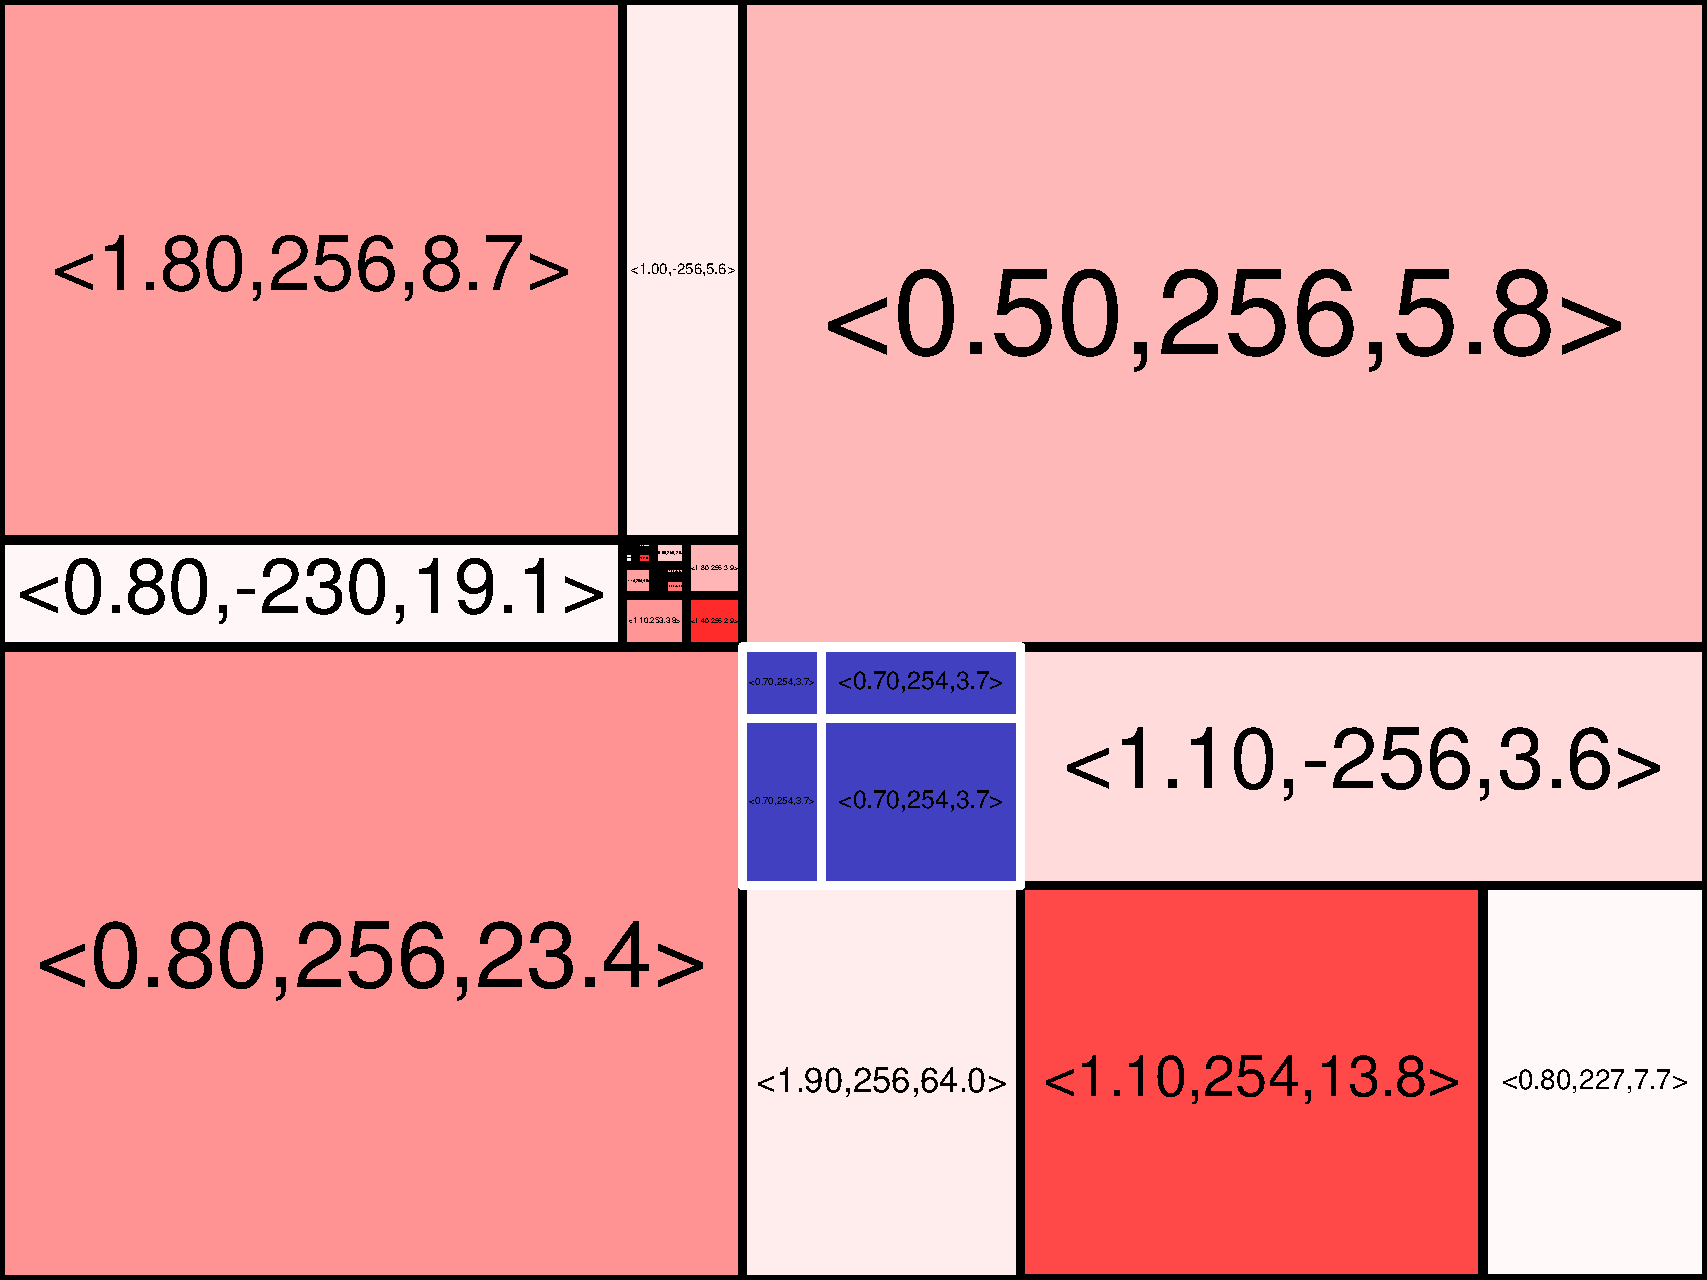
\includegraphics[width=8.5 cm]{remy-graph/graph/test26.pdf}

\end{centering}\end{frame}


\begin{frame}
\frametitle{Iterate}\begin{centering}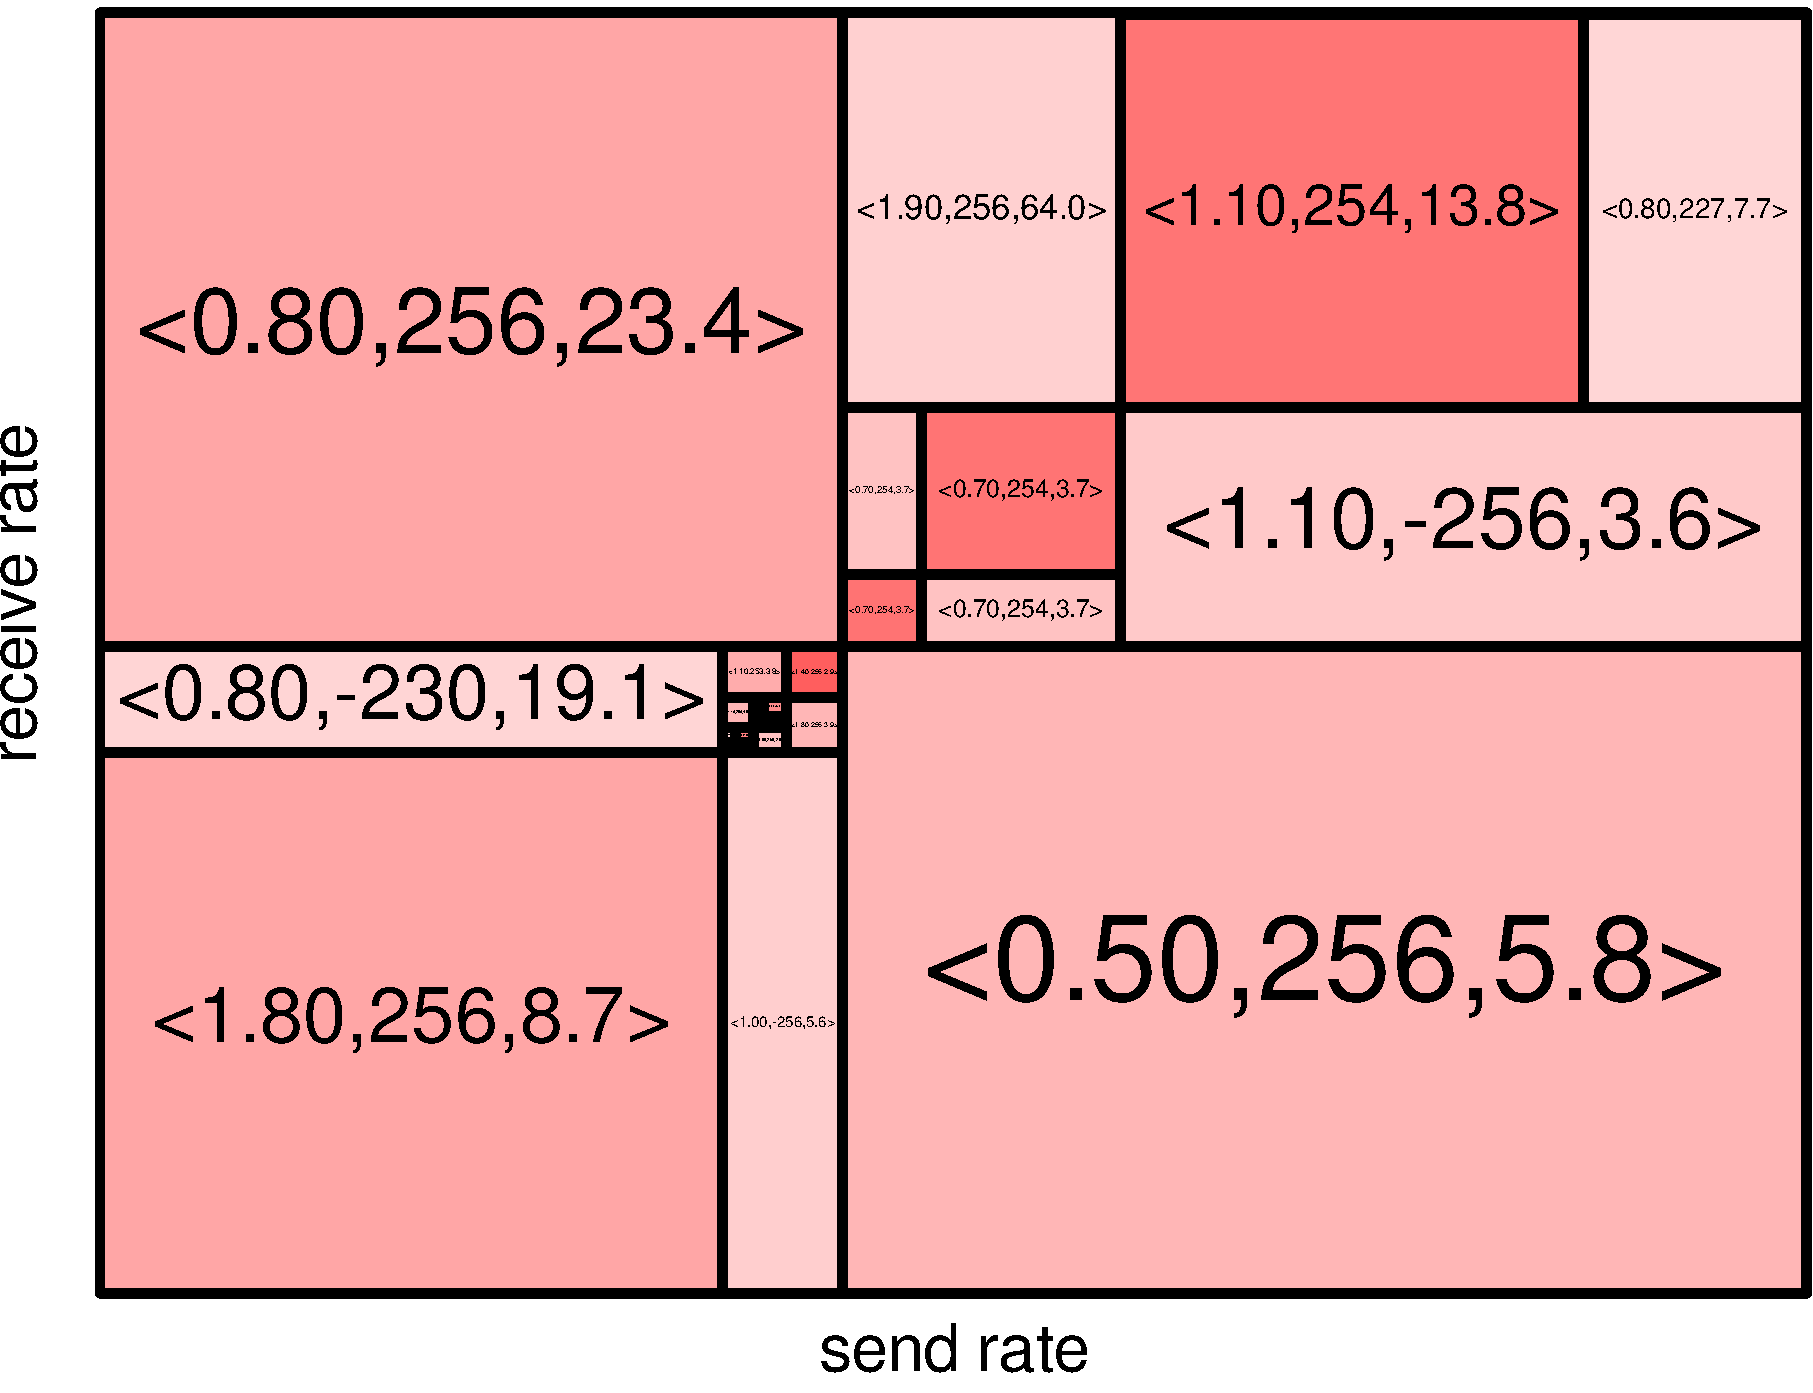
\includegraphics[width=8.5 cm]{remy-graph/graph/test27.pdf}

\end{centering}\end{frame}


\begin{frame}
\frametitle{Iterate}\begin{centering}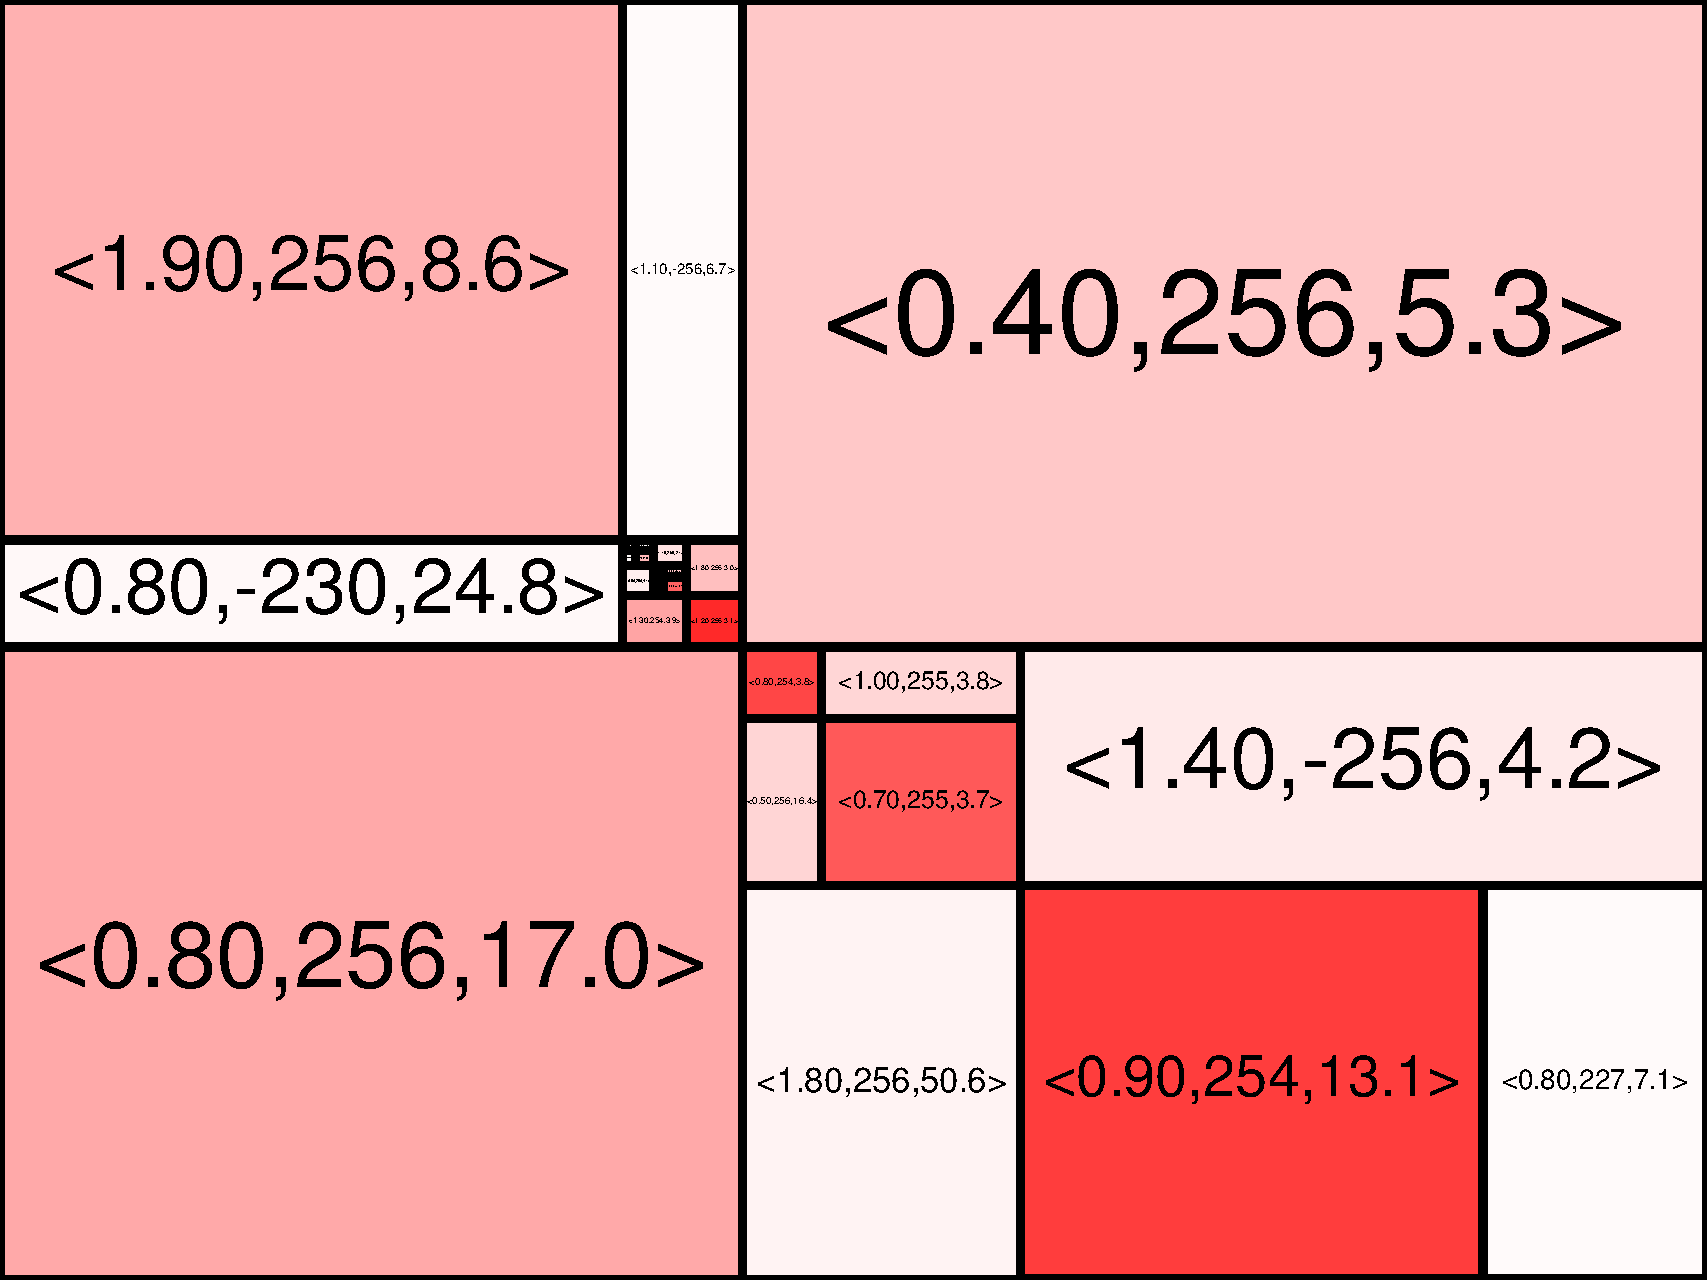
\includegraphics[width=8.5 cm]{remy-graph/graph/test28.pdf}

\end{centering}\end{frame}


\begin{frame}
\frametitle{Iterate}\begin{centering}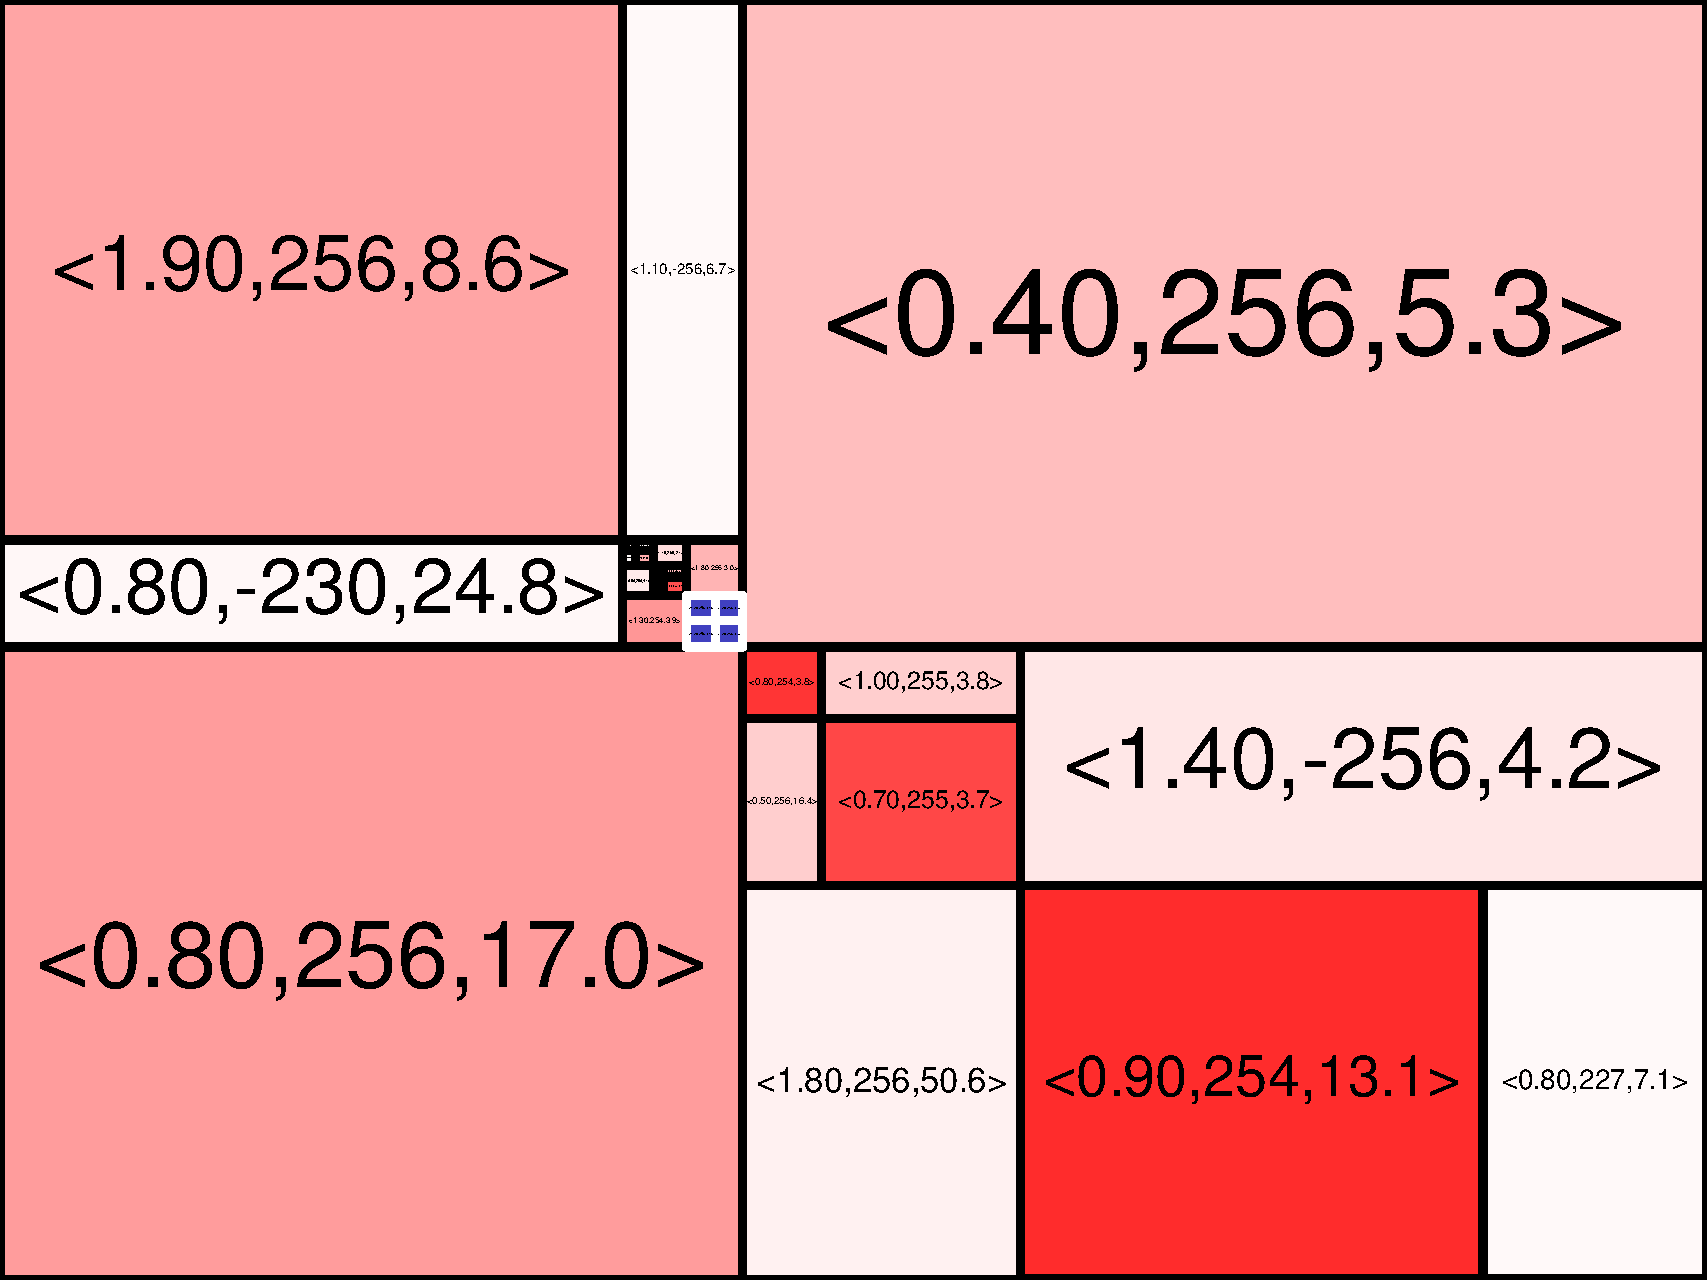
\includegraphics[width=8.5 cm]{remy-graph/graph/test29.pdf}

\end{centering}\end{frame}


\begin{frame}
\frametitle{Iterate}\begin{centering}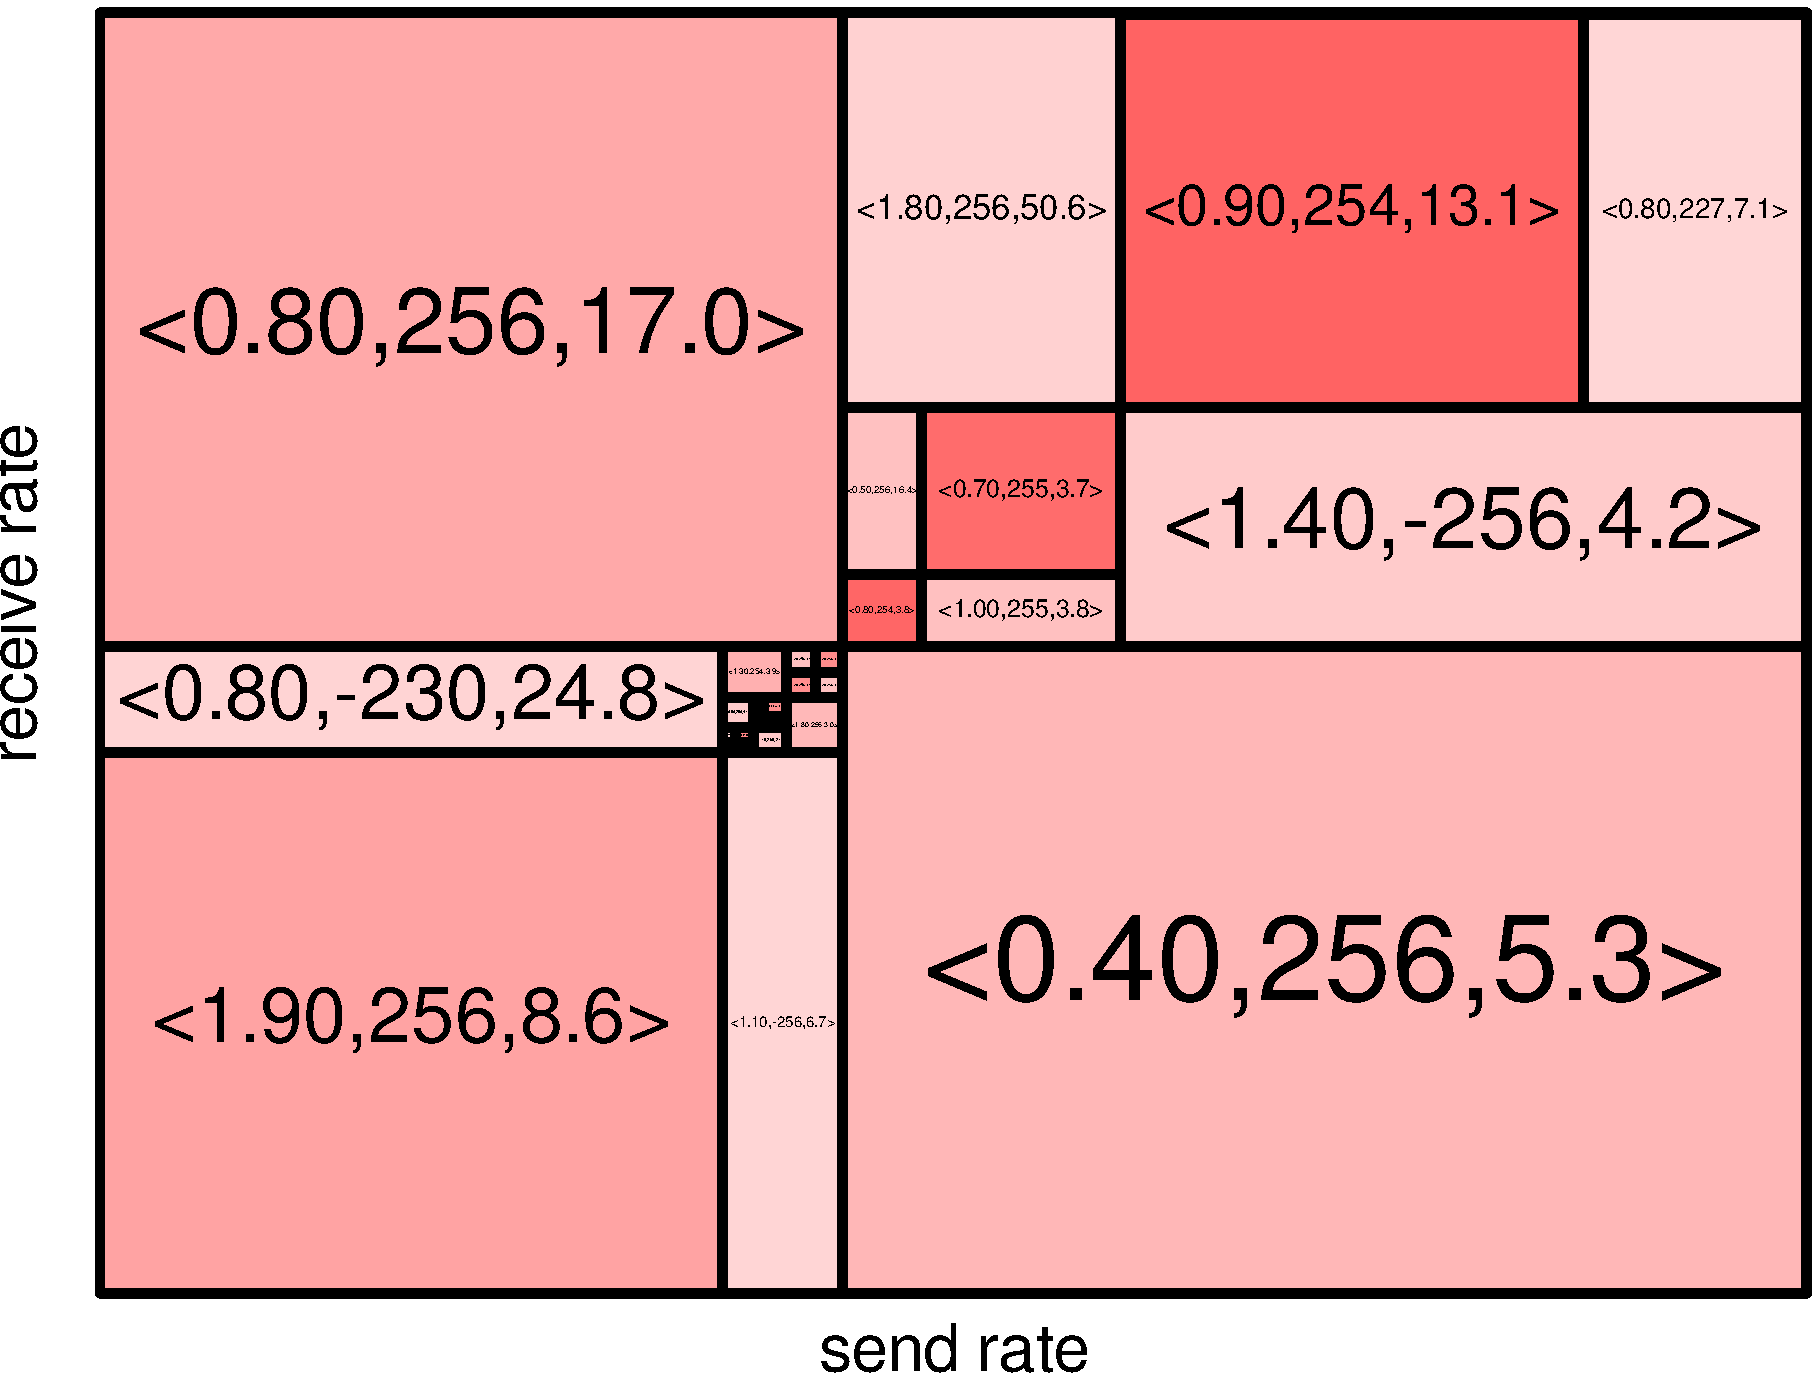
\includegraphics[width=8.5 cm]{remy-graph/graph/test30.pdf}

\end{centering}\end{frame}


\begin{frame}
\frametitle{Iterate}\begin{centering}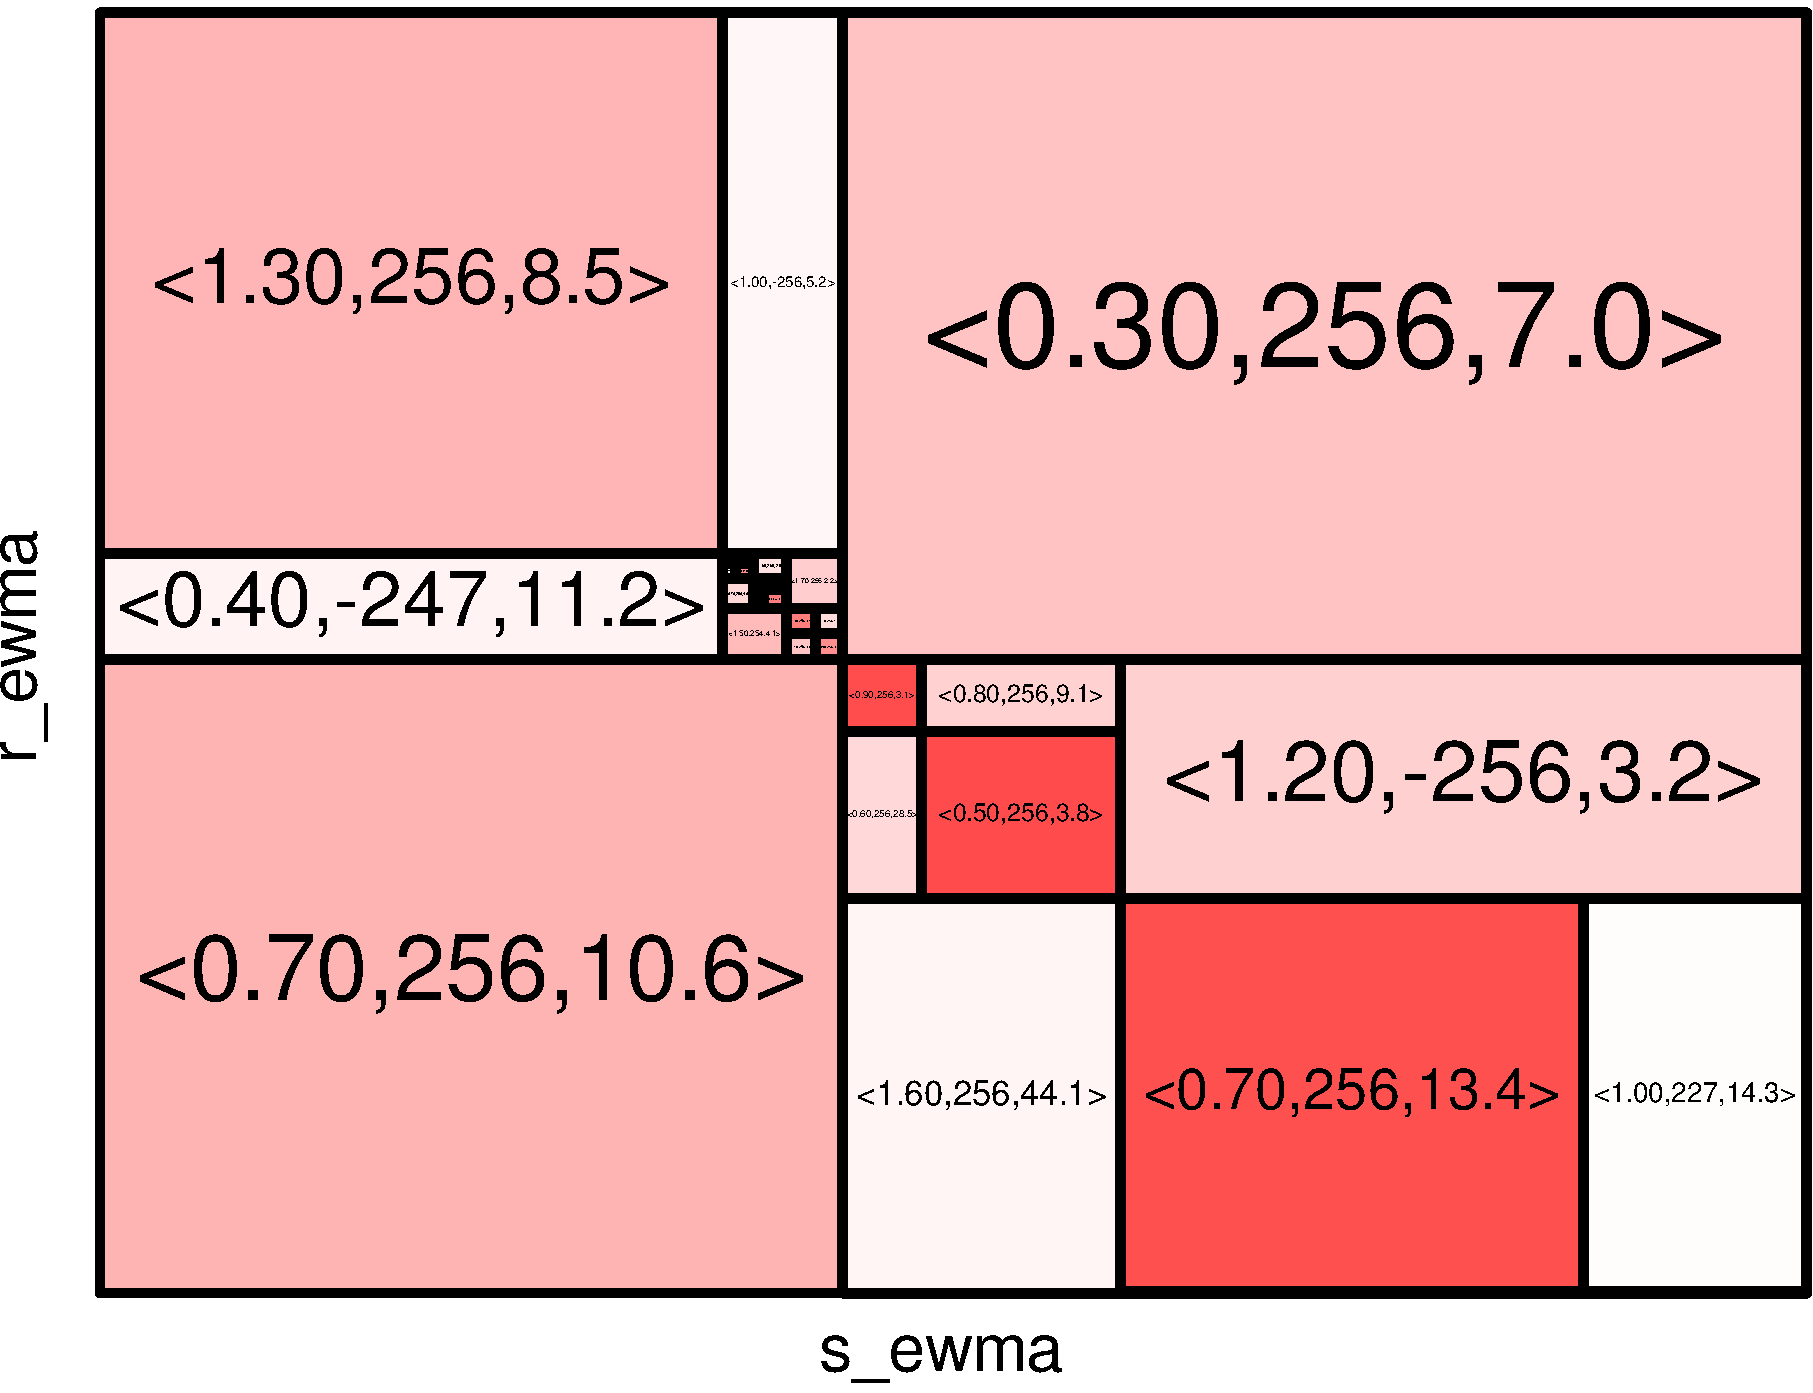
\includegraphics[width=8.5 cm]{remy-graph/graph/test31.pdf}

\end{centering}\end{frame}


\begin{frame}
\frametitle{Iterate}\begin{centering}\includegraphics[width=8.5 cm]{remy-graph/graph/test32.pdf}

\end{centering}\end{frame}


\begin{frame}
\frametitle{Iterate}\begin{centering}\includegraphics[width=8.5 cm]{remy-graph/graph/test33.pdf}

\end{centering}\end{frame}


\begin{frame}
\frametitle{Iterate}\begin{centering}\includegraphics[width=8.5 cm]{remy-graph/graph/test34.pdf}

\end{centering}\end{frame}


\begin{frame}
\frametitle{Iterate}\begin{centering}\includegraphics[width=8.5 cm]{remy-graph/graph/test35.pdf}

\end{centering}\end{frame}


\begin{frame}
\frametitle{Iterate}\begin{centering}\includegraphics[width=8.5 cm]{remy-graph/graph/test36.pdf}

\end{centering}\end{frame}


\begin{frame}
\frametitle{Iterate}\begin{centering}\includegraphics[width=8.5 cm]{remy-graph/graph/test37.pdf}

\end{centering}\end{frame}


\begin{frame}
\frametitle{Iterate}\begin{centering}\includegraphics[width=8.5 cm]{remy-graph/graph/test38.pdf}

\end{centering}\end{frame}


\begin{frame}
\frametitle{Iterate}\begin{centering}\includegraphics[width=8.5 cm]{remy-graph/graph/test39.pdf}

\end{centering}\end{frame}


\begin{frame}
\frametitle{Iterate}\begin{centering}\includegraphics[width=8.5 cm]{remy-graph/graph/test40.pdf}

\end{centering}\end{frame}


\begin{frame}
\frametitle{Iterate}\begin{centering}\includegraphics[width=8.5 cm]{remy-graph/graph/test41.pdf}

\end{centering}\end{frame}


\begin{frame}
\frametitle{Iterate}\begin{centering}\includegraphics[width=8.5 cm]{remy-graph/graph/test42.pdf}

\end{centering}\end{frame}


\begin{frame}
\frametitle{Iterate}\begin{centering}\includegraphics[width=8.5 cm]{remy-graph/graph/test43.pdf}

\end{centering}\end{frame}


\begin{frame}
\frametitle{Iterate}\begin{centering}\includegraphics[width=8.5 cm]{remy-graph/graph/test44.pdf}

\end{centering}\end{frame}


\begin{frame}
\frametitle{Iterate}\begin{centering}\includegraphics[width=8.5 cm]{remy-graph/graph/test45.pdf}

\end{centering}\end{frame}


\begin{frame}
\frametitle{Iterate}\begin{centering}\includegraphics[width=8.5 cm]{remy-graph/graph/test46.pdf}

\end{centering}\end{frame}


\begin{frame}
\frametitle{Iterate}\begin{centering}\includegraphics[width=8.5 cm]{remy-graph/graph/test47.pdf}

\end{centering}\end{frame}


\begin{frame}
\frametitle{Iterate}\begin{centering}\includegraphics[width=8.5 cm]{remy-graph/graph/test48.pdf}

\end{centering}\end{frame}


\begin{frame}
\frametitle{Iterate}\begin{centering}\includegraphics[width=8.5 cm]{remy-graph/graph/test49.pdf}

\end{centering}\end{frame}


\begin{frame}
\frametitle{Iterate}\begin{centering}\includegraphics[width=8.5 cm]{remy-graph/graph/test50.pdf}

\end{centering}\end{frame}


\begin{frame}
\frametitle{Iterate}\begin{centering}\includegraphics[width=8.5 cm]{remy-graph/graph/test51.pdf}

\end{centering}\end{frame}


\begin{frame}
\frametitle{Iterate}\begin{centering}\includegraphics[width=8.5 cm]{remy-graph/graph/test52.pdf}

\end{centering}\end{frame}


\begin{frame}
\frametitle{Iterate}\begin{centering}\includegraphics[width=8.5 cm]{remy-graph/graph/test53.pdf}

\end{centering}\end{frame}


\begin{frame}
\frametitle{Iterate}\begin{centering}\includegraphics[width=8.5 cm]{remy-graph/graph/test54.pdf}

\end{centering}\end{frame}


\begin{frame}
\frametitle{Iterate}\begin{centering}\includegraphics[width=8.5 cm]{remy-graph/graph/test55.pdf}

\end{centering}\end{frame}


\begin{frame}
\frametitle{Iterate}\begin{centering}\includegraphics[width=8.5 cm]{remy-graph/graph/test56.pdf}

\end{centering}\end{frame}


\begin{frame}
\frametitle{Iterate}\begin{centering}\includegraphics[width=8.5 cm]{remy-graph/graph/test57.pdf}

\end{centering}\end{frame}


\begin{frame}
\frametitle{Iterate}\begin{centering}\includegraphics[width=8.5 cm]{remy-graph/graph/test58.pdf}

\end{centering}\end{frame}


\begin{frame}
\frametitle{Iterate}\begin{centering}\includegraphics[width=8.5 cm]{remy-graph/graph/test59.pdf}

\end{centering}\end{frame}


\begin{frame}
\frametitle{Iterate}\begin{centering}\includegraphics[width=8.5 cm]{remy-graph/graph/test60.pdf}

\end{centering}\end{frame}


\begin{frame}
\frametitle{Iterate}\begin{centering}\includegraphics[width=8.5 cm]{remy-graph/graph/test61.pdf}

\end{centering}\end{frame}


\begin{frame}
\frametitle{Iterate}\begin{centering}\includegraphics[width=8.5 cm]{remy-graph/graph/test62.pdf}

\end{centering}\end{frame}


\begin{frame}
\frametitle{Iterate}\begin{centering}\includegraphics[width=8.5 cm]{remy-graph/graph/test63.pdf}

\end{centering}\end{frame}


\begin{frame}
\frametitle{Iterate}\begin{centering}\includegraphics[width=8.5 cm]{remy-graph/graph/test64.pdf}

\end{centering}\end{frame}


\begin{frame}
\frametitle{Iterate}\begin{centering}\includegraphics[width=8.5 cm]{remy-graph/graph/test65.pdf}

\end{centering}\end{frame}


\begin{frame}
\frametitle{Iterate}\begin{centering}\includegraphics[width=8.5 cm]{remy-graph/graph/test66.pdf}

\end{centering}\end{frame}


\begin{frame}
\frametitle{Iterate}\begin{centering}\includegraphics[width=8.5 cm]{remy-graph/graph/test67.pdf}

\end{centering}\end{frame}


\begin{frame}
\frametitle{Iterate}\begin{centering}\includegraphics[width=8.5 cm]{remy-graph/graph/test68.pdf}

\end{centering}\end{frame}


\begin{frame}
\frametitle{Iterate}\begin{centering}\includegraphics[width=8.5 cm]{remy-graph/graph/test69.pdf}

\end{centering}\end{frame}


\begin{frame}
\frametitle{Iterate}\begin{centering}\includegraphics[width=8.5 cm]{remy-graph/graph/test70.pdf}

\end{centering}\end{frame}


\begin{frame}
\frametitle{Iterate}\begin{centering}\includegraphics[width=8.5 cm]{remy-graph/graph/test71.pdf}

\end{centering}\end{frame}


\begin{frame}
\frametitle{Iterate}\begin{centering}\includegraphics[width=8.5 cm]{remy-graph/graph/test72.pdf}

\end{centering}\end{frame}


\begin{frame}
\frametitle{Iterate}\begin{centering}\includegraphics[width=8.5 cm]{remy-graph/graph/test73.pdf}

\end{centering}\end{frame}


\begin{frame}
\frametitle{Iterate}\begin{centering}\includegraphics[width=8.5 cm]{remy-graph/graph/test74.pdf}

\end{centering}\end{frame}


\begin{frame}
\frametitle{Iterate}\begin{centering}\includegraphics[width=8.5 cm]{remy-graph/graph/test75.pdf}

\end{centering}\end{frame}


\begin{frame}
\frametitle{Iterate}\begin{centering}\includegraphics[width=8.5 cm]{remy-graph/graph/test76.pdf}

\end{centering}\end{frame}


\begin{frame}
\frametitle{Iterate}\begin{centering}\includegraphics[width=8.5 cm]{remy-graph/graph/test77.pdf}

\end{centering}\end{frame}


\begin{frame}
\frametitle{Iterate}\begin{centering}\includegraphics[width=8.5 cm]{remy-graph/graph/test78.pdf}

\end{centering}\end{frame}


\begin{frame}
\frametitle{Iterate}\begin{centering}\includegraphics[width=8.5 cm]{remy-graph/graph/test79.pdf}

\end{centering}\end{frame}


\begin{frame}
\frametitle{Iterate}\begin{centering}\includegraphics[width=8.5 cm]{remy-graph/graph/test80.pdf}

\end{centering}\end{frame}


\begin{frame}
\frametitle{Iterate}\begin{centering}\includegraphics[width=8.5 cm]{remy-graph/graph/test81.pdf}

\end{centering}\end{frame}


\begin{frame}
\frametitle{Iterate}\begin{centering}\includegraphics[width=8.5 cm]{remy-graph/graph/test82.pdf}

\end{centering}\end{frame}


\begin{frame}
\frametitle{Iterate\hspace{10 cm}.}\begin{centering}\includegraphics[width=8.5 cm]{remy-graph/graph/test83.pdf}

\end{centering}\end{frame}


\begin{frame}
\frametitle{Iterate\hspace{10 cm}.}\begin{centering}\includegraphics[width=8.5 cm]{remy-graph/graph/test84.pdf}

\end{centering}\end{frame}


\begin{frame}
\frametitle{Iterate\hspace{10 cm}.}\begin{centering}\includegraphics[width=8.5 cm]{remy-graph/graph/test85.pdf}

\end{centering}\end{frame}


\begin{frame}
\frametitle{Iterate}\begin{centering}\includegraphics[width=8.5 cm]{remy-graph/graph/test86.pdf}

\end{centering}\end{frame}


\begin{frame}
\frametitle{Iterate\hspace{10 cm}*}\begin{centering}\includegraphics[width=8.5 cm]{remy-graph/graph/test87.pdf}

\end{centering}\end{frame}


\begin{frame}
\frametitle{Iterate}\begin{centering}\includegraphics[width=8.5 cm]{remy-graph/graph/test88.pdf}

\end{centering}\end{frame}


\begin{frame}
\frametitle{Evaluation in ns-2}

\section{Evaluation}

\begin{itemize}

\item End-to-end comparators: \textcolor{Red}{NewReno, Cubic, Compound, Vegas}

\item In-net comparators: \textcolor{DarkGreen}{Cubic-over-sfqCoDel, XCP, DCTCP}

\item Simulation setup published for replication

\end{itemize}

\begin{centering}
\includegraphics[width=9 cm]{reproducethis.png}

\end{centering}

\end{frame}

\begin{frame}
\frametitle{Scenario 1: fixed-rate network, homogenous senders}

\includegraphics[width=\textwidth]{dumbbell.pdf}

\end{frame}

\begin{frame}
\frametitle{Scenario 1: details}

\begin{tabular}{lllll}
\bf Quantity & & \bf Simulation parameter & \bf Remy assumptions \\

\hline Link speed & & 15~Mbps & Uniform(10, 20)~Mbps \\

RTT & & 150~ms & Uniform(100, 200)~ms \\

$n$ & & 8 & Uniform(1, 16) \\

``On'' process & & $\mathrm{exp}[\mu = 100]\,\textbf{\textcolor{DarkBlue}{kB}}$ & $\mathrm{exp}[\mu = 5]\,\textbf{\textcolor{DarkBlue}{s}}$ \\

``Off'' process & & $\mathrm{exp}\left[\mu = \textcolor{DarkBlue}{\bm {\frac{1}{2}}}\right]\,\textsf{s}$ & $\mathrm{exp}[\mu = \textcolor{DarkBlue}{\bm 5} ]\,\textsf{s}$ \\

\end{tabular}

\ssline
\ssline

\textbf{Remy objective:} \[\sum_i \log \left[ \frac{\textsf{throughput}_i}{\big(\textsf{delay}_i\big)^{\textcolor{DarkBlue}{{\bm \delta}}}} \right]\]

\[\textcolor{DarkBlue}{{\bm \delta}} \in \bigg\{ \frac{1}{10}, 1, 10 \bigg\} \]

\end{frame}

\begin{frame}
\frametitle{Scenario 1: throughput-delay plot}

\begin{centering}
\only<1>{\includegraphics[width=8.5 cm]{eth8-annotated-11.pdf}}\only<2>{\includegraphics[width=8.5 cm]{eth8-annotated-10.pdf}}\only<3>{\includegraphics[width=8.5 cm]{eth8-annotated-9.pdf}}\only<4>{\includegraphics[width=8.5 cm]{eth8-annotated-8.pdf}}\only<5>{\includegraphics[width=8.5 cm]{eth8-annotated-7.pdf}}\only<6>{\includegraphics[width=8.5 cm]{eth8-annotated-6.pdf}}\only<7>{\includegraphics[width=8.5 cm]{eth8-annotated-7.pdf}}\only<8>{\includegraphics[width=8.5 cm]{eth8-annotated-5.pdf}}\only<9>{\includegraphics[width=8.5 cm]{eth8-annotated-4.pdf}}\only<10>{\includegraphics[width=8.5 cm]{eth8-annotated-3.pdf}}\only<11>{\includegraphics[width=8.5 cm]{eth8-annotated-1.pdf}}\only<12>{\includegraphics[width=8.5 cm]{eth8-annotated.pdf}}

\end{centering}
\end{frame}

\begin{frame}
\frametitle{Scenario 2: $n = 12$, heavy-tailed flow lengths}

\begin{centering}
\includegraphics[width=8.5 cm]{eth12-final-flowcdf.pdf}

\end{centering}

\end{frame}

\begin{frame}
\frametitle{Scenario 3: Verizon LTE, $n = 8$}

\begin{centering}
\includegraphics[width=8.5 cm]{vzw-8-final.pdf}

\end{centering}
\end{frame}

\begin{frame}
\frametitle{Scenario 4: data center}

\textbf{Throughput (Mbps):}

\begin{tabular}{lll}
&  Mean &  Median \\
 DCTCP (ECN) & \cellcolor{Green} 179 & 144 \\
 RemyCC (DropTail) & 175 & \cellcolor{Green} 158 \\
% RemyCC+RED & 102,  & \\
\vspace{\baselineskip}
\end{tabular}

\ssline
\ssline

\textbf{RTT (ms):}

\begin{tabular}{lll}
&  Mean &  Median \\
 DCTCP (ECN) & \cellcolor{Green}{7.5} & \cellcolor{Green}{6.4} \\
 RemyCC (DropTail) & {34} & {39} \\
%\bf RemyCC+RED & 102,  & \\
\vspace{\baselineskip}
\end{tabular}

\end{frame}

\begin{frame}
\frametitle{Scenario 5: heterogenous traffic}

\begin{itemize}
\item Standing queue from cross traffic can't be solved end-to-end
\item But can keep up in throughput if included in assumptions
\end{itemize}

\ssline

\begin{tabular}{lll}
\bf Mean off time & \bf RemyCC tput & \bf Compound tput \\
\hline 200 ms & \cellcolor{Green} 2.12 (.11)~Mbps & 1.79 (.18)~Mbps \\
100 & 2.18 (.08)  & \cellcolor{Green} 2.75 (.27) \\
10 & 2.28 (.10) & \cellcolor{Green} 3.9 (.13) \\
\\
\\
\bf Mean size & \bf RemyCC tput & \bf Cubic tput \\
\hline
100 KBytes & \cellcolor{Green} 2.04 (.14) & 1.31 (.16)\\
1 MByte & \cellcolor{Green} 2.09 (.11) & 1.28 (.11) \\
\end{tabular}

\end{frame}

\begin{frame}
\frametitle{Prior knowledge is helpful, when correct}

\begin{centering}
\includegraphics[width=8.5 cm]{spec2.pdf}

\end{centering}

\end{frame}

\begin{frame}

\frametitle{Our work}
\section{Discussion}

\begin{centering}

\LARGE \textcolor{DarkGreen}{If congestion control is the answer,\\what's the question?}

\vspace{\baselineskip}

\LARGE \textcolor{NavyBlue}{Are there better answers?}

\end{centering}

\end{frame}

\begin{frame}
\frametitle{Key limitations}

\begin{itemize}
\item Tested only in simulation so far

\item[]

\item To get the right answer, have to ask the right question

\item[]

\item Don't know how to characterize robustness to the unforeseen

\item[]

\item End-to-end = hard to handle an overaggressive competitor

\item[]

\item Do we need more congestion signals to broaden range?

\end{itemize}

\end{frame}

\begin{frame}
\frametitle{Goal-driven algorithm \textbf{moves} the complexity}

\textbf{Human-designed algorithm:}

\begin{itemize}
\item Simple algorithm
\item Variable and subpar emergent behavior
\item[] \ldots worse when \textcolor{DarkBlue}{implicit assumptions} not met
\end{itemize}

\textbf{Computer-designed algorithm:}

\begin{itemize}
\item Complex algorithm
\item More consistent and better behavior
\item[] \ldots worse when \textcolor{DarkBlue}{stated assumptions} not met
\end{itemize}

\end{frame}

\begin{frame}
\frametitle{Surprises}

\LARGE

\begin{itemize}

\item \textcolor{DarkGreen}{Computer-designed} {\LARGE \textbf{\textgreater}} \textcolor{DarkRed}{human-designed}

\item[]

\item \textcolor{DarkGreen}{End-to-end} {\LARGE \textbf{\textgreater}} \textcolor{DarkRed}{in-network{\LARGE \textbf{*}}}

\item[]

\item[] \hspace{6.0 cm}\normalsize\textcolor{DarkRed}{{\bf *} (so far)}

\end{itemize}

\end{frame}

\begin{frame}
\frametitle{Acknowledgments}

\begin{centering}
\begin{tabular}{lll}
Anirudh Sivaraman & Ranjita Bhagwan \\
Leslie Kaelbling & Christopher Amato \\
Scott Shenker & Frans Kaashoek \\
Nickolai Zeldovich & Damon Wischik \\
Chris Lesniewski & Juliusz Chroboczek \\
\end{tabular}

\end{centering}

\ssline
\ssline

\footnotesize We thank the members of the MIT Center for Wireless
Networks and Mobile Computing (Wireless@MIT), including Amazon.com,
Cisco, Google, Intel, Mediatek, Microsoft, ST Microelectronics, and
Telefonica, for their support. KW was supported by the Claude
E.~Shannon Research Assistantship. This work was also supported in
part by NSF grant CNS-1040072.

\end{frame}

\begin{frame}
\frametitle{Conclusions}

\large

\begin{itemize}

\item The network evolves. Transport should let it!

\item[]

\item Computer-designed schemes can outperform humankind's best so far.

\item[]

\item Let's focus on the question---that's the hard part anyway.

\end{itemize}

\ssline

\begin{centering}

\textcolor{DarkBlue}{http://web.mit.edu/remy}

\vspace{\baselineskip}

\{keithw,hari\}@mit.edu

\end{centering}

\end{frame}

\end{document}
